% !Mode:: "Tex:UTF-8"

%\chapter{Diseño de experimentos}
%
%\section*{\fbox{\colorbox{Gris025}{{Sesión 27. Diseño experimental.}}}}\label{sesion:27}
%
%\subsection*{\fbox{\colorbox{Gris025}{{Análisis de la varianza.}}}}
%\subsection*{Fecha: Martes, 10/01/2012, 14h.}
%
%\noindent{\bf Atención: este fichero pdf lleva adjuntos los ficheros de datos necesarios.}
%
%%\subsection*{\fbox{1. Ejemplos preliminares }}
%\setcounter{tocdepth}{1}
%%\tableofcontents

\section{Un modelo $C\sim F$ sencillo.}

En este capítulo vamos a estudiar inicialmente el caso más sencillo del problema que, en la Tabla
\ref{tabla:MetodosInferencia2Variables} (pág. \pageref{tabla:MetodosInferencia2Variables}) hemos
llamado $C \sim F$. En este tipo de problemas la variable respuesta es una variable cuantitativa
(por lo tanto, un número), mientras que la variable explicativa es un factor (variable
cualitativa).  El siguiente es un ejemplo típico de esta situación, que vamos a ir desarrollando a
lo largo del capítulo para que nos sirva como introducción al tema.

\begin{ejemplo}
\label{cap11:ejem:Anova01}
Después de tratar con éxito la depresión en los canguros rojos australianos (recuerda el Ejemplo
\ref{cap07:ejem:CangurosDepresivos01} del Capítulo \ref{cap:ContrasteHipotesis}), el laboratorio
creador de {\em Pildorín Complex} ha decidido ampliar su cartera de clientes, y está investigando
el alicaimiento en el Frailecillo Común {\em Fratercula arctica}, ver Figura
\ref{cap11:fig:Frailecillo})

\begin{figure}[htbp]
\begin{center}
\begin{enColor}
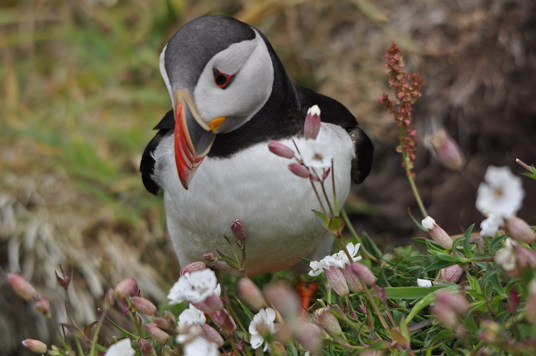
\includegraphics[width=10cm]{../fig/Cap11-FrailecilloAlicaido.png}
\end{enColor}
\begin{bn}
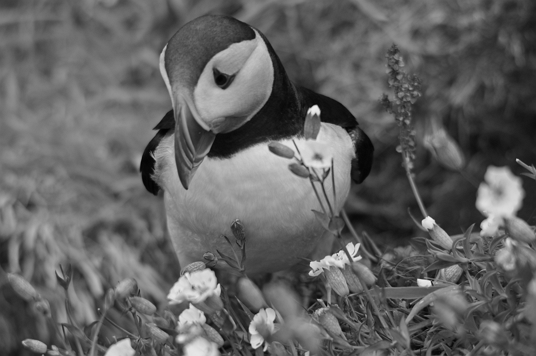
\includegraphics[width=10cm]{../fig/Cap11-FrailecilloAlicaido-bn.png}
\end{bn}
\caption{Un frailecillo, bastante alicaído el pobre.}
\label{cap11:fig:Frailecillo}
\end{center}
\end{figure}

Para tratar esta dolencia, el laboratorio ha encargado a cuatro de sus mejores investigadores que
desarrollen tratamientos para los frailecillos. Tras meses de arduos trabajos en sus laboratorios,
los equipos presentan sus resultados, que son cuatro tratamientos distintos:
\begin{itemize}
  \item {\em Alirón plus.}
  \item {\em Vuelagra.}
  \item {\em Plumiprofeno.}
  \item {\em Elevantolín.}
\end{itemize}
Naturalmente, el laboratorio tiene que decidir cuál va a ser su apuesta: ¿cuál de estos es el mejor tratamiento? En la fase de prueba, se seleccionan cuatro muestras aleatorias independientes de
100 frailecillos alicaídos cada una, y se tratan esas muestras con cada uno de los cuatro tratamientos que compiten. Minuciosamente, los experimentadores encargados de las comprobaciones miden la frecuencia de aleteo (en aleteos por minuto) de cada uno de los frailecillos que han sido tratados, y anotan los 400 resultados (cuatro tratamientos, cien frailecillos para cada uno). El resultado será una tabla, que en muchos casos tendrá el aspecto de nuestra Tabla \ref{cap11:tabla:DefectuosaEjemploAnova01}, de la que sólo mostramos las seis primeras filas (tiene 100 filas de números):
\begin{table}[ht]
\begin{center}
\begin{minipage}{10cm}
\begin{verbatim}
          Aliron Elevantolin  Plumiprofeno Vuelagra
        1  76.65       88.66         87.14    76.74
        2  79.36       78.12         82.34    74.72
        3  71.83       81.74         94.06    68.61
        4  73.24       89.11         88.12    72.84
        5  79.73       82.90         84.47    75.83
        6  74.50       80.84         83.11    66.81
\end{verbatim}
\end{minipage}
\end{center}
\caption{Tabla defectuosa del Ejemplo \ref{cap11:ejem:Anova01}.}
\label{cap11:tabla:DefectuosaEjemploAnova01}
\end{table}
Pero, antes de seguir adelante, un ruego: lee, en el Tutorial11, cuál es la mejor manera de
almacenar en un fichero los datos de un estudio como este. No es una buena idea guardarlos imitando
la estructura de la Tabla \ref{cap11:tabla:DefectuosaEjemploAnova01}.

Hay dos variables que intervienen en esta tabla. Por un lado, el {\em tratamiento}, que es una
variable cualitativa, un factor, con cuatro niveles, los cuatro medicamentos que estamos
comparando, y que en este caso se corresponden con las columnas de la tabla. Y por otro lado, la
{\em respuesta} del frailecillo al tratamiento, que es una variable cuantitativa, un número (que se
mide en aleteos/minuto).

Queremos elegir el mejor tratamiento. Para conseguirlo,  ¿cuál es la pregunta que queremos
contestar con estos datos? Se trata de saber, para empezar, si hay {\em diferencias significativas}
entre los tratamientos (si todos ellos fueran básicamente iguales, con diferencias insignificantes,
el laboratorio elegiría el más barato o usaría algún otro criterio).

Ya habrás sospechado que las palabras ``diferencias significativas'', que hemos destacado en el
anterior párrafo, no son casuales, y apuntan hacia un contraste entre dos hipótesis. Enseguida
daremos los detalles técnicos, pero el resultado de esta primera fase será una decisión entre la
hipótesis nula ``los tratamientos son todos iguales'' y la hipótesis alternativa ``no lo son'' (esto {\em no} significa que sean todas distintas unas de otras; más adelante discutiremos esto con más detalle).

En una segunda fase, si hemos (rechazado la hipótesis nula y) confirmado que hay diferencias
significativas, trataremos de decidir cuál es el mejor. En esa segunda fase buscamos un resultado
como ``Alirón y Plumiprofeno son esencialmente iguales, pero ambos son mejores que Vuelagra o
Elevantolín''. Pero ya llegaremos ahí. Primero tenemos que dar más precisiones sobre la primera
fase. \qed
\end{ejemplo}


En el método Anova que vamos a ver en este capítulo, se acostumbra a usar la terminología de {\sf
tratamiento}\index{tratamiento, variable en Anova} y {\sf respuesta}\index{respuesta, variable en
Anova} para las variables cualitativa (factor) y cuantitativa, respectivamente. Incluso cuando el
significado de esas variables no tiene nada que ver con ``tratamientos''. Por ejemplo, si estamos
estudiando los retrasos medios en los vuelos de cuatro compañías aéreas, podríamos decir que el
{\em tratamiento} es la variable ``compañía aérea''. Y en este ejemplo hemos visto los ingredientes
básicos del problema que nos va a ocupar en este capítulo. Queremos estudiar la posible relación
entre dos variables, del tipo $C \sim F$, donde la variable cuantitativa $X$, la que llamamos {\tt
respuesta}, se relaciona con la variable explicativa, un factor al que llamamos {\sf tratamiento}.

Para estudiar esa posible relación, nuestro plan pasa, como siempre, por hacer estas dos cosas:
supondremos que la distribución de las variables cumple ciertas condiciones y tomaremos muestras
para estimar los parámetros del problema. Empecemos por la distribución de las variables.

\subsubsection{Condiciones teóricas sobre la distribución de las variables}

Tenemos, por tanto, la variable {\em tratamiento}, $T$, que es un factor,
y vamos a suponer que tiene $k$ niveles.
\[t_1, t_2, \ldots, t_k.\]
A menudo llamaremos también {\em tratamientos} a cada uno de los niveles del factor tratamiento. La notación es un poco ambigua, pero no suele generar confusión. En el Ejemplo \ref{cap11:fig:Frailecillo} los niveles son cuatro, y corresponden a cada uno de los medicamentos que probamos. Puesto que queremos comparar la respuesta frente a esos tratamientos, una manera de verlo es pensar que estamos frente a $k$ poblaciones distintas e independientes,
donde la primera población corresponde a los casos tratados con $t_1$, el primer nivel del tratamiento, la segunda población a los casos tratados con $t_2$, etc. Y estudiamos la respuesta $X$ en esas $k$ poblaciones, así que estamos pensando en $k$ variables independientes
\[X_1, X_2, \ldots, X_k.\]
Por ejemplo, la variable $X_2$ representa la respuesta de la población al nivel $t_2$ del tratamiento. Como puedes ver, estamos haciendo una identificación entre la población y el nivel $t_k$ del tratamiento.

Al pensarlo así, podemos ver este problema como una generalización del estudio de la diferencia de medias $\mu_1-\mu_2$, en dos poblaciones normales, que vimos en la Sección \ref{cap09:sec:diferenciaMediasDosPoblaciones} (pág. \pageref{cap09:sec:diferenciaMediasDosPoblaciones}) del Capítulo \ref{cap:Inferencia2Poblaciones}. Recordemos que allí estudiábamos una misma variable $X$ en dos poblaciones independientes, en las que $X$ tenía distribución normal:
    \[
    X_1\sim N\left(\mu_1,\sigma_1\right),
    \quad\mbox{ y }\quad
    X_2\sim N\left(\mu_2,\sigma_2\right).\]
Podemos generalizar este problema a un número cualquiera $k\geq 2$ de poblaciones, cada una con su distribución normal.
 \[
    X_1\sim N\left(\mu_1,\sigma\right),
    \quad
    X_2\sim N\left(\mu_2,\sigma\right),
    \,\ldots,\,
    X_k\sim N\left(\mu_k,\sigma\right).
 \]
Pero, además, en esta generalización hemos introducido una condición adicional, que va a ser importante para nuestro trabajo en todo este capítulo:
\paragraph*{}\label{cap11:lugar:homocedasticidad}
        \fcolorbox{black}{Gris025}{
        \begin{minipage}{12cm}
        \begin{center}
        {\bf Homogeneidad de varianzas}
        \end{center}
            {\sf Vamos a suponer que la desviación típica $\sigma$ es la misma en todos los
            niveles del tratamiento (poblaciones).}
        \end{minipage}}\\[3mm]
Esta condición se llama técnicamente {\sf homocedasticidad}\index{homocedasticidad en Anova}. Recuerda que ese término ya  apareció en la Sección \ref{cap10:subsec:modeloRegresionLinealSimple}, (pág. \pageref{cap10:subsec:modeloRegresionLinealSimple}), y que también lo hemos llamado, de forma más sencilla, {\sf homogeneidad de las varianzas}\index{homogeneidad de las varianzas en Anova}.

En el Ejemplo \ref{cap11:fig:Frailecillo} hemos visto también que, en una primera fase, queremos comparar la media de la variable respuesta frente a los distintos niveles del tratamiento. Vamos a suponer que las medias de los valores de $X$ correspondientes a cada uno de esos niveles del tratamiento (es decir, en cada una de las poblaciones) son:
    \[\mu_1,\mu_2,\ldots,\mu_k.\]
Entonces, como primer paso, queremos contrastar la hipótesis nula
        \begin{equation}\label{cap11:ecu:HipotesisNulaAnova}
            H_0=\{\mu_1=\mu_2=\cdots=\mu_k\}.
        \end{equation}
Esta hipótesis nula indica que no hay diferencias significativas en la respuesta producida por los distintos niveles del tratamiento. Es decir, no hay relación significativa entre la respuesta $X$ y el tratamiento $T$, por decirlo en el lenguaje de un modelo como $X\sim T$.

Un detalle de notación: puesto que en la hipótesis nula \ref{cap11:ecu:HipotesisNulaAnova} todas las medias son iguales, cuando sea necesario llamaremos $\mu_0$ a ese valor común de la media. Y una observación a tener en cuenta. La hipótesis alternativa correspondiente a la hipótesis nula \ref{cap11:ecu:HipotesisNulaAnova} no es ``todas las medias son distintas unas de otras''. No, la hipótesis alternativa correcta es ``por lo menos hay dos medias distintas entre todas las medias $\mu_1$,\ldots,$\mu_k$''. Insistimos, para que $H_0$ sea falsa, basta con que haya dos medias distintas en ese conjunto de medias.

\subsection{Muestras y notación para el modelo.}
\label{cap10:subsec:MuestrasNotacionModelo}

Como de costumbre, para estimar $\mu_1,\ldots,\mu_k$, y contrastar la hipótesis nula $H_0$, tenemos que tomar muestras. Concretamente, vamos a tomar $k$ muestras aleatorias simples e independientes, una por cada nivel del tratamiento (esto es, una por población). En el lenguaje de las pruebas de medicamentos, eso quiere decir a cada uno de los $k$ niveles del tratamiento disponibles le hemos asignado un cierto grupo de pacientes. Vamos a llamar $n_j$ al número de pacientes que se han asignado al nivel $t_j$ del tratamiento, donde $j$ va desde 1 hasta $k$.

Si llamamos $X(i,j)=x_{ij}$ al valor de la variable $X$ en el paciente número $i$ del grupo número $j$, entonces, como hicimos en la Tabla \ref{cap11:tabla:DefectuosaEjemploAnova01}  del Ejemplo \ref{cap11:ejem:Anova01}, podemos anotar los resultados experimentales en forma de tabla:
\begin{table}[ht]
\[
        \begin{array}{cccccc}
        &\multicolumn{5}{r}\mbox{\bf Nivel del Tratamiento ($j$ de 1 a $k$)}\\
        \cline{2-6}
        &t_1&t_2&t_3&\cdots&t_k\\
        \hline
                                &x_{11}&x_{12}&x_{13}&\cdots&x_{1k}\\
   \mbox{\bf Respuestas}        &x_{21}&x_{22}&x_{23}&\cdots&x_{2k}\\
   \mbox{\bf ($i$ de 1 a $n_j$)}&x_{31}&x_{32}&x_{33}&\cdots&x_{3k}\\
                                &\vdots&\vdots&\vdots&\ddots&\vdots\\
                                &x_{n_11}&x_{n_22}&x_{n_33}&\cdots&x_{n_kk}\\
        \hline
        \end{array}
\]
\caption{Tabla muestral para Anova.}
\label{cap11:tabla:Anova01}
\end{table}
Algunas observaciones importantes sobre la notación:
\begin{itemize}
    \item No queremos ponernos muy pesados con la notación, pero es importante ser cuidadosos para que, en el futuro, no provoque imprecisiones y llegue a convertirse en un estorbo. Pero si no entiendes de que hablamos en el resto de este punto, no te preocupes, y pasa al siguiente de la lista; quedará más claro en el Tutorial11, al hacer las cuentas con el ordenador. Hemos escrito
        \[X(i,j)=x_{i,j}\]
        para indicar que los {\em argumentos} de la variable $X$ son los números enteros $i$ y $j$, que nos dicen, en el caso de $j$, a qué nivel del factor (o número de población) nos referimos o, en el caso de $i$, a cuál de los elementos de la muestra nos referimos. Así que $X(3,2)$ nos indica el tercer elemento de la muestra del segundo nivel del tratamiento, que es lo que, con otra notación, llamamos $x_{3,2}$ (en otras palabras, el tercer paciente al que se le ha aplicado el tratamiento número $2$).

  \item Aunque la tabla anterior parece indicar que todos los tratamientos han sido probados en el mismo número de pacientes, {\em en general no es así}, de modo que cada columna de la Tabla (\ref{cap11:tabla:Anova01}) puede tener distinta longitud. Es decir, {\em no estamos suponiendo} que sea $n_1=n_2=\cdots=n_k$. Si eso sucede, y todas las muestras son del mismo tamaño, diremos que se trata de un {\sf diseño equilibrado}\index{diseño equilibrado en Anova}\index{equilibrado, diseño en Anova} (en inglés, {\em balanced}).

  \item Llamaremos $N$ al total de observaciones que se han hecho, para el conjunto de niveles del tratamiento, de manera que:
      \[N=n_1+n_2+\cdots+n_k.\]
  \item Además, conviene comprobar, cuando se usan las fórmulas de un libro de texto, cuáles son los significados de $i$ y $j$ en $x_{ij}$, porque algunos autores los cambian de orden. Nosotros vamos a utilizar la notación más coherente con la notación matricial, de uso general en Matemáticas, en la que, en una tabla, $i$ indica la fila, y $j$ indica la columna.
  \item Ya hemos dicho, en el Ejemplo \ref{cap11:ejem:Anova01}, que aunque esta notación nos ayuda conceptualmente en las explicaciones del modelo, no es desde luego la más conveniente para nuestro trabajo con el ordenador. Nos remitimos al Tutorial11 para los detalles pertinentes.
\end{itemize}


\begin{ejemplo}{\bf (Continuación del Ejemplo \ref{cap11:ejem:Anova01}).}
\label{cap11:ejem:Anova01a}
En el ejemplo de los frailecillos, tenemos $k=4$ niveles del tratamiento, que se corresponden a cuatro poblaciones. Por ejemplo la descripción de la primera población es: ``los frailecillos alicaídos a los que se trata con {\em Alirón plus}''. Y de esa población hemos tomado una muestra aleatoria de 100 individuos, en los que hemos obtenido los valores de las respuestas:
\[
x_{1,1}= 76.65,\,\, x_{2,1}=79.36,\,\, x_{3,1}=71.83,\, \ldots,\, x_{99,1}=83.85,\,\, x_{100,1}= 83.84
\]
Como ves, usamos una coma en los subíndices cuando conviene, para evitar ambigüedades. Son los valores de la primera columna de la Tabla \ref{cap11:tabla:DefectuosaEjemploAnova01} (pág. \pageref{cap11:tabla:DefectuosaEjemploAnova01}). En este ejemplo se tiene $N=400$, con
\[n_1=n_2=n_3=n_4=100\]
así que estamos ante lo que hemos llamado un diseño equilibrado.
\qed
\end{ejemplo}
Una vez recogidas las muestras, estamos listos para el contraste, y para entender por qué, a lo que vamos a hacer, se le llama Anova, y qué tiene que ver con la idea de análisis o descomposición de la varianza que ya vimos en el modelo de regresión lineal simple (Sección \ref{cap10:sec:AnovaCoeficienteCorrelacion}, pág. \pageref{cap10:sec:AnovaCoeficienteCorrelacion}).

\section{Residuos e identidad Anova.}
\label{cap11:sec:ResiduosIdentidadAnova}

El método que vamos a describir, y que se conoce como Anova de un factor (luego precisaremos la terminología),  permite realizar el contraste de la hipótesis nula de igualdad de medias (Ecuación \ref{cap11:ecu:HipotesisNulaAnova} (pág. \pageref{cap11:ecu:HipotesisNulaAnova}), mediante una identidad de descomposición o análisis de la varianza, similar a la Identidad Anova \ref{cap10:ecu:AnovaparaRegresion} (pág. \pageref{cap10:ecu:AnovaparaRegresion}), que vimos en el Capítulo \ref{cap:RegresionLinealSimple}  para el caso de la regresión lineal.

Para hacer algo similar, en el problema que nos ocupa en este capítulo, necesitamos algo más de notación. Usaremos la notación que se usa en muchos textos de estadística para estos problemas, porque es necesario que el lector esté familiarizado con ella.

Con esa notación, para representar la suma de valores del grupo $j$ (columna $j$ de la Tabla \ref{cap11:tabla:Anova01}) se utiliza el símbolo:
        \[X_{\colorbox{lightgrey}{\mbox{\bf\large$\cdot$}}j}=\sum_{i=1}^{n_j}x_{ij}\]
Observa el punto que aparece como subíndice (y que, en esta ocasión, hemos sombreado en gris para destacarlo). Ese punto indica sumación sobre la variable $i$ a la que sustituye. Por ejemplo, la media de la muestra número $j$ sería
          \[
          \bar X_{{\mbox{\bf\large$\cdot$}}j}	=
          \dfrac{X_{{\mbox{\bf\large $\cdot$}}j}}{n_j},
          \]
Y la suma de todos los valores de la tabla se indicará con dos puntos:
    \[X_{{\mbox{\bf\large $\cdot\cdot$}}}=\sum_{j=1}^k\sum_{i=1}^{n_j}x_{ij}.\]
La media de todos los valores muestrales de la tabla se indica simplemente colocando una barra sobre $X$, como hemos hecho en otros capítulos:
    \[\bar{X}=\dfrac{X_{{\mbox{\bf\large $\cdot\cdot$}}}}{N}.\]

\begin{ejemplo}{\bf (Continuación del Ejemplo \ref{cap11:ejem:Anova01a}, pág. \pageref{cap11:ejem:Anova01a}).}
\label{cap11:ejem:FrailecillosCalculoMediasGrupos}

 En el ejemplo de los frailecillos se tiene:
\[
\begin{cases}
\bar X_{{\mbox{\bf\large$\cdot$}}1}=78.40,&
\mbox{ respuesta media muestral para $t_1$, {Aliron Plus}}.\\
\bar X_{{\mbox{\bf\large$\cdot$}}4}=80.40,&
\mbox{ respuesta media  muestral para $t_4$, {Elevantolin}}.\\
\bar X_{{\mbox{\bf\large$\cdot$}}3}=84.40,&
\mbox{ respuesta media  muestral para $t_3$, {Plumiprofeno}}.\\
\bar X_{{\mbox{\bf\large$\cdot$}}2}=72.10,&
\mbox{ respuesta media muestral  para $t_2$, {Vuelagra}}.

\end{cases}
\]
y la media muestral total es
\[\bar{X}=78.82.\]
\qed
\end{ejemplo}

Con esta notación, empecemos el trabajo necesario para obtener el contraste de igualdad de medias. Dado cualquier valor $x_{ij}$ de la Tabla \ref{cap11:tabla:Anova01} (pág. \pageref{cap11:tabla:Anova01}) podemos escribir esta igualdad:
    \begin{equation}
    \label{cap11:ecu:AnovaIdentidadEstimadores}
        x_{ij}-\bar X=
        (x_{ij}-\bar X_{\mbox{\bf\large $\cdot$}j})+
        (\bar X_{\mbox{\bf\large$\cdot$}j}-\bar X)
    \end{equation}
Esta ecuación es el primer paso hacia lo que queremos hacer. Antes de seguir, pensemos lo que significa esto en el ejemplo.

\begin{ejemplo}{\bf (Continuación del Ejemplo \ref{cap11:ejem:FrailecillosCalculoMediasGrupos}).}
\label{cap11:ejem:FrailecillosCalculoMediasGrupos-a}
Vamos a pensar en uno de los frailecillos tratados con $t_3$, Plumiprofeno. Es decir, su respuesta al tratamiento aparece en la columna $3$ de la Tabla \ref{cap11:tabla:DefectuosaEjemploAnova01}. Supongamos que nos fijamos en el de la cuarta fila. Su respuesta, como puedes ver en esa tabla, es
\[x_{4,3}=88.12\]
La respuesta media (muestral) de todos los frailecillos que hemos observado es, como hemos visto antes, $\bar{X}=78.82$. Así pues la diferencia entre la respuesta individual de este frailecillo y la respuesta media (de los 400) es:
\[x_{4,3}  - \bar X = 88.12 - 78.82 = 9.3,\]
así que podemos decir que a este frailecillo en concreto el tratamiento le ha ido bastante mejor que a la media. Para explicar esa mejoría, descomponemos este valor $9.3$ en la suma de dos contribuciones. Por un lado, calculamos la diferencia:
\[(\bar X_{\mbox{\bf\large$\cdot$}4}-\bar X)=  1.58\]
Este valor se obtiene usando sólo el hecho de que el frailecillo ha sido tratado con $t_4$,  Plumiprofeno. Y no depende, {\em esto es esencial}, de las circunstancias individuales que intervienen en el tratamiento de ese frailecillo en particular. El número es el mismo para todos los frailecillos tratados con $t_4$.

Para medir la contribución de esas circunstancias individuales, calculamos el residuo, que es el término
\[(x_{4,3}-\bar X_{\mbox{\bf\large $\cdot$}3})= 7.72,\]
que mide cómo de diferente es la respuesta de este frailecillo comparada con la respuesta media los del mismo grupo de tratamiento.

Naturalmente, los tres números que hemos obtenido cumplen:
\[9.3 = 7.72 + 1.58\]
Pero lo interesante es la interpretación de estos números. Esta ecuación nos dice que, de los 9.3 puntos que diferencian a este frailecillo concreto de la media, hay $1.58$ puntos que podemos atribuir al tratamiento con Plumiprofeno, y $7.72$ puntos que se deben a características individuales del tratamiento en el caso de este frailecillo. Puede ser que este individuo tenga una especial predisposición genética que hace que el tratamiento resulte, en él, especialmente efectivo. O puede ser que su alicaimiento ha remitido por otras causas (se ha echado novia, o ha descubierto un banco de arenques especialmente sabrosos y nutritivos, etc.)
\end{ejemplo}

A la luz de este ejemplo, retomamos la discusión. El valor $\bar X$ es un estimador de $\mu_0$, que es la media que aparece en la hipótesis nula, mientras que cada una de las medias de grupo $\bar X_{\mbox{\bf\large $\cdot$}j}$ es un estimador del valor $\mu_j$ (para $j=1,\ldots,k$). Y recordemos que esa hipótesis nula dice que no hay diferencias entre los niveles del tratamiento, así que todas las diferencias entre respuestas que observemos son {\em fruto del azar}, o del {\em ruido}, con la terminología que ya conocemos. Es decir, que si una respuesta individual $x_{ij}$ es distinta de $\mu_0$, es por causa de eso que estamos llamando {\em azar o ruido}. Nosotros, en la Ecuación \ref{cap11:ecu:AnovaIdentidadEstimadores}, hemos descompuesto esa respuesta como suma de dos contribuciones:
\begin{itemize}
  \item El término $e_{ij}=(x_{ij}-\bar X_{\mbox{\bf\large $\cdot$}j})$, al que vamos a llamar el {\sf residuo}\index{residuo en Anova} de esa respuesta individual. Va a jugar un papel análogo al de los residuos (Ecuación \ref{cap10:ecu:ResiduosRegresionLineal}, pág. \pageref{cap10:ecu:ResiduosRegresionLineal}) en la regresión lineal.
  \item El término $(\bar X_{\mbox{\bf\large$\cdot$}j}-\bar X)$, que no depende de $i$, sólo de $j$, {\em así que su valor es el mismo para todas las respuestas de la muestra tratada con $t_j$}.
\end{itemize}
Esta última observación, como hemos visto en el ejemplo, es la clave de la interpretación de los términos que componen esta igualdad.  Pero antes de hacer la interpretación, vamos a hacer una observación esencial, que nos permite pasar de la discusión de individuos a la discusión sobre toda la información muestral en su conjunto. Se trata de una identidad de suma de cuadrados, análoga a la  Ecuación \ref{cap10:ecu:AnovaparaRegresion} (pág. \pageref{cap10:ecu:AnovaparaRegresion}) que vimos en el Capítulo \ref{cap:RegresionLinealSimple}:\\[1mm]

    \fcolorbox{black}{Gris025}{
        \begin{minipage}{12cm}
        \begin{center}
        {\bf Identidad de la suma de cuadrados para Anova}
        \index{identidad de la suma de cuadrados para Anova de un factor}
        \index{Anova de un factor, identidad de la suma de cuadrados}
        \end{center}
        \begin{equation}\label{cap11:ecu:identidadSumaCuadradosAnova}
        \underbrace{\sum_{j=1}^k\sum_{i=1}^{n_j}(x_{ij}-\bar X)^2}_{SST}=
        \underbrace{\sum_{j=1}^k\sum_{i=1}^{n_j}(x_{ij}-\bar X_{\mbox{\bf\large
        $\cdot$}j})^2}_{SS_{\mbox{\tiny residual}}}
        +
        \underbrace{\sum_{j=1}^k \colorbox{lightgrey}{$n_j$}(\bar X_{\mbox{\bf\large $\cdot$}j}-\bar X)^2}_{SS_{\mbox{\tiny modelo}}}
        \end{equation}
        Es decir $\displaystyle SST= SS_{\mbox{\tiny residual}} + SS_{\mbox{\tiny modelo}}$.
        \end{minipage}
    }\\[3mm]
Fíjate en el $n_j$ que aparece en el tercer término, y que hemos destacado. Representa, como sabemos, el número de elementos de cada muestra.

El análisis de la varianza consiste en la interpretación de cada uno de los tres términos de esta
ecuación, que hemos llamado $SST$, $SS_{\mbox{\tiny residual}}$ y $SS_{\mbox{\tiny modelo}}$,  como
ya hicimos en el caso de la regresión lineal. Veamos cómo se interpreta aquí cada uno de ellos:
        \begin{itemize}
        \item El primer término, que hemos llamado $SST$,  representa la dispersión total de los datos cuando se consideran como si procedieran de una única población combinada, sin hacer diferencias entre los niveles del tratamiento. Entonces, cada respuesta individual se compara con la media $\bar X$ del conjunto muestral completo.
        \item El tercer término $SS_{\mbox{\tiny modelo}}$ representa la dispersión en los datos
            que se atribuye al hecho de que se utilizan $k$ tratamientos distintos. Es la {\sf
            dispersión entre grupos}\index{entre grupos, dispersión en Anova de un
            factor}\index{dispersión entre grupos en Anova de un factor}, o también diremos que
            es la parte de la dispersión o varianza {\em explicada por el modelo} (de ahí la $E$,
            de {\em explained}). En algunos libros se usa también la notación $SSB$ para este
            término, donde la $B$ proviene del inglés {\em between}, y se dice que es la variación {\em
            entre} grupos.
        \item El segundo término $SS_{\mbox{\tiny residual}}$ representa la dispersión en los
            datos que se atribuye al factor aleatorio, al {\em azar o ruido}. Se suele decir que
            esta es la  {\sf dispersión dentro de los grupos}\index{dispersión dentro de los
            grupos, Anova de un factor} o intra-grupo, porque se debe a las circunstancias
            individuales de cada aplicación de un nivel del tratamiento, y por tanto a razones
            que en este modelo se consideran aleatorias. La notación alternativa para este
            término es $SSW$, donde la $W$ proviene del inglés {\em within}, y se dice que es la
            variación {\em dentro} de los grupos.
        \end{itemize}
De nuevo, en este caso sigue siendo válida la advertencia sobre la notación $SS$ que  hicimos en el Capítulo \ref{cap:RegresionLinealSimple} (ver página \pageref{cap10:parag:AdvertenciaSSE})


Para reforzar la interpretación de cada término que hemos descrito, podemos razonar de una forma similar a la que usamos en el caso de la regresión lineal: supongamos que no existiera ningún {\em ruido}, y que por tanto el azar no interviene para hacer a unas respuestas individuales distintas de otras. Entonces, {\em la diferencia entre respuestas se debería exclusivamente al nivel del tratamiento empleado. Todas las respuestas, dentro de una misma muestra, serían exactamente iguales entre sí, e iguales a la media del grupo.}

Con la notación que estamos usando, eso significa que $x_{ij}=\bar X_{\mbox{\bf\large $\cdot$}j}$
(para todos los niveles $j=1,\ldots,k$). Así que
\[SS_{\mbox{\tiny residual}}=0,\]
y la identidad Anova implica que, en ese caso, se tiene:
\[SST=  SS_{\mbox{\tiny modelo}}.\]
Es decir, que no hay ruido aleatorio, y la variación que observamos queda completamente explicada por el modelo. La situación es análoga a la de la Figura \ref{cap10:fig:Anova01} (pág. \pageref{cap10:fig:Anova01}), en la que la recta (el modelo) predecía exactamente la posición de los puntos. Aquí el papel de la recta lo ejercen los valores $\bar X_{\mbox{\bf\large $\cdot$}j}$.

Veamos como funciona la identidad en nuestro ejemplo.
\begin{ejemplo}{\bf (continuación del Ejemplo \ref{cap11:ejem:Anova01})}
\label{cap11:ejem:Anova01e}

Como veremos en el Tutorial11, para el ejemplo de los frailecillos se obtiene, usando el ordenador:
\[SST=14881.38,\quad  SS_{\mbox{\tiny modelo}} = 7896.76, \quad  SS_{\mbox{\tiny residual}} = 6984.41,\]
Puedes comprobar que $SS_{\mbox{\tiny modelo}}+SS_{\mbox{\tiny residual}}=14881.17$, que no
coincide exactamente con $SST$ por un pequeño margen, debido al redondeo en las operaciones
numéricas que hace el programa (si se usara un programa simbólico la coincidencia sería perfecta).

Ahora podemos usar estos números para reproducir, a escala de toda la muestra, la discusión que
antes hacíamos para un frailecillo individual. De la dispersión total, igual a $14881.38$, podemos
atribuir una parte considerable $SS_{\mbox{\tiny modelo}} = 7896.76$ a los efectos del tratamiento.
Esta es la parte de la dispersión explicada por el modelo $X\sim T$ que estamos analizando. La
contribución del azar es la suma de cuadrados residuales $SS_{\mbox{\tiny residual}}=6984.41$, que
representa a la parte de la dispersión que queda sin explicar por ese modelo.

Por cierto, ¿en qué unidades están esas medidas de dispersión, como el $14881.38$ de la dispersión total? Un momento de reflexión nos hará ver que están, nada menos, en (aleteos/minuto)$^2$.
\qed
\end{ejemplo}

\section{El estadístico del contraste y la tabla Anova.}
\label{cap11:sec:EstadisticoContrasteTablaAnova}

La identidad Anova \ref{cap11:ecu:identidadSumaCuadradosAnova} nos permite cuantificar, y medir de una forma precisa, cual es la parte de la dispersión en la muestra que se puede atribuir al modelo $X  \sim T$ que estamos analizando, y que parte es fruto del azar. Pero, como ya hemos visto en otros casos similares, para que esa medición sea útil, es necesario obtener un valor que no dependa de las dimensiones y de las escalas de medición particulares del problema. Hemos aprendido, en los anteriores capítulos, que esa medida adimensional es la que permite, además, obtener un estadístico cuyo comportamiento corresponda a alguna de las distribuciones clásicas de probabilidad.

El remedio es el mismo que ya hemos aplicado en otras ocasiones. Dividimos toda la identidad de
suma de cuadrados Anova por el término $SS_{\mbox{\tiny residual}}$:
\[SST = SS_{\mbox{\tiny residual}} + SS_{\mbox{\tiny modelo}},\]
obteniendo:
\[
\dfrac{SST}{SS_{\mbox{\tiny residual}}}= 1 + \dfrac{SS_{\mbox{\tiny modelo}}}{SS_{\mbox{\tiny residual}}}
\]
El término en el que nos vamos a fijar es el que tiene que ver con la parte de la dispersión explicada por el modelo $X \sim T$, que es, concretamente:
    \[
    \dfrac{SS_{\mbox{\tiny modelo}}}{SS_{\mbox{\tiny residual}}}=
    \dfrac{\displaystyle\sum_{j=1}^k n_j\cdot(\bar X_{\mbox{\bf\large $\cdot$}j}-\bar X)^2}
    {\sum_{j=1}^k\sum_{i=1}^{n_j}(x_{ij}-\bar X_{\mbox{\bf\large
        $\cdot$}j})^2}.
    \]

No vamos a explicar en detalle el siguiente paso, y desde luego no vamos a dar una demostración rigurosa, pero sí podemos tratar de justificar informalmente lo que haremos. La idea es que, estudiando el comportamiento muestral de las dos cantidades que aparecen aquí, por un lado:
\[\sum_{j=1}^k n_j\cdot(\bar X_{\mbox{\bf\large $\cdot$}j}-\bar X)^2
\quad\mbox{ y por otro }\quad
    \sum_{j=1}^k\sum_{i=1}^{n_j}(x_{ij}-\bar X_{\mbox{\bf\large
        $\cdot$}j})^2,
    \]
y manteniendo el objetivo de tipificar para hacer aparecer la distribución normal, podemos hacer algunas
manipulaciones para escribir $\frac{SS_{\mbox{\tiny modelo}}}{SS_{\mbox{\tiny residual}}}$ como un
cociente, cuyo numerador $SS_{\mbox{\tiny modelo}}$ y denominador $SS_{\mbox{\tiny residual}}$ son
{\em ambos} sumas de una cierta cantidad de normales estándar al cuadrado. Es decir, que el
numerador y denominador son, cada uno de ellos, una cierta distribución $\chi^2$. Y ya sabemos,
porque apareció en el Capítulo \ref{cap:Inferencia2Poblaciones}, que el cociente de
dos $\chi^2$ se comporta como una distribución $F$ de Fisher. El lector interesado en los detalles técnicos puede encontrarlos en el Capítulo 11
del libro \cite{inferenciaIpinnaDurand},  o presentados de otra manera en el Capítulo 16 del libro
\cite{garcia2009estadistica}. En particular, ahí se encuentra la justificación detallada de los grados de libertad de $F$ que vamos a utilizar. Nosotros volveremos sobre eso más adelante, con una justificación más informal.

En las operaciones anteriores, y en el resultado que vamos a presentar, juega un papel importante el hecho de que el diseño muestral es, como hemos dicho, {\em equilibrado}, de manera que todas las muestras, para los distintos niveles del tratamiento, son del mismo tamaño. En ese caso, el resultado es este:\\[3mm]
    \fcolorbox{black}{Gris025}{
    \begin{minipage}{13cm}
    \begin{center}
    {\bf Distribución muestral de los componentes del Anova unifactorial}\\
    {\bf para el caso de un modelo equilibrado.}\\
    \end{center}
    Supongamos que la hipótesis nula \ref{cap11:ecu:HipotesisNulaAnova} (pág.
    \pageref{cap11:ecu:HipotesisNulaAnova})
    \[H_0=\{\mu=\mu_1=\mu_2=\cdots=\mu_k\}\]
    es cierta, y el diseño es equilibrado con $k$ niveles del tratamiento, todos del mismo
    tamaño, $n_1=n_2=\cdots=n_k$, que llamaremos $n$. Entonces:
    \begin{equation}\label{cap11:ecu:distribucionMuestralAnova1Fequilibrado}
    \Xi=\dfrac{\dfrac{SS_{\mbox{\tiny modelo}}}{k-1}}{\dfrac{SS_{\mbox{\tiny residual}}}{N-k}}
    =
    \dfrac{\quad
    n\cdot\dfrac{\sum_{j=1}^k (\bar X_{\mbox{\bf\large $\cdot$}j}-\bar X)^2}{k-1}
    \quad
    }{
    \quad\dfrac{\sum_{j=1}^k\sum_{i=1}^{n_j}(x_{ij}-\bar X_{\mbox{\bf\large
    $\cdot$}j})^2}{N-k}\quad
    }\sim F_{k-1;N-k}
    \end{equation}
    siendo $F_{k-1;N-k}$ la distribución de Fisher-Snedecor con $k-1$ y $N-k$ grados de
    libertad. Recuerda que $N$ es el total de observaciones, así que en el diseño equilibrado es
    $N=k\cdot n$.
    \end{minipage}
    }\\[3mm]
Este resultado puede parecer complicado, pero el mensaje es el que ya hemos discutido en las anteriores secciones. Al calcular el estadístico:
\[
\Xi=\dfrac{\dfrac{SS_{\mbox{\tiny modelo}}}{k-1}}{\dfrac{SS_{\mbox{\tiny residual}}}{N-k}}
\]
estamos, salvo por el embrollo técnico de los grados de libertad, comparando los tamaños de, por un lado,  la parte $SS_{\mbox{\tiny modelo}}$ de la dispersión, que consideramos explicada por el modelo $X \sim T$, y por otro lado, la dispersión $SS_{\mbox{\tiny residual}}$, que consideramos debida al azar. Si la hipótesis nula es
cierta, todas las diferencias entre niveles del tratamiento se deben al azar, y el modelo $X\sim T$
no debería ser capaz de explicar apenas nada de la dispersión. Obtendríamos un resultado cercano al
0. Por contra, si la fracción que representa $SS_{\mbox{\tiny modelo}}$ es suficientemente grande,
quien defienda la validez de la hipótesis nula se verá en un apuro para explicar ese valor tan alto
del cociente. En resumen, son los valores grandes, los de la cola derecha de la distribución del
estadístico $\Xi$, los que nos van a llevar a rechazar la hipótesis nula de igualdad de medias entre
los distintos niveles del tratamiento.

La forma habitual de presentar los cálculos del contraste de igualdad de medias en el modelo Anova que hemos descrito, es mediante lo que se denomina una {\sf tabla Anova}\index{tabla Anova}\index{Anova, tabla} como la Tabla \ref{cap11:tabla:Anova02}.

\setlength{\tabcolsep}{5pt}
\begin{center}
\begin{table}[ht]
    \begin{tabular}{@{}l@{\quad} c c c @{}c@{} c}
    \hline
    {\small Fuente de}&{\small Suma de}&{\small Grados de}&{\small Cuadrado}&{\small Estadístico}&{\small
    {\bf p-valor}}\\
    {\small variación}&{\small cuadrados}&{\small libertad}&{\small medio}& &\\
    \hline
    $SS_{\mbox{\tiny modelo}}$&{\small $n\cdot\displaystyle\sum_{j=1}^k (\bar X_{\mbox{\bf\large $\cdot$}j}-\bar X)^2$}&$k-1$&{\small $\dfrac{n\cdot \displaystyle\sum_{j=1}^k (\bar X_{\mbox{\bf\large $\cdot$}j}-\bar X)^2}{k-1}$}&$\Xi$&{$\mathbf{P(F>\Xi)}$ }\\[3mm]

    $SS_{\mbox{\tiny residual}}$&{\small $\displaystyle\sum_{j=1}^k\sum_{i=1}^{n_j}(x_{ij}-\bar X_{\mbox{\bf\large $\cdot$}j})^2$}&$n-k$&{\small $\dfrac{\displaystyle\sum_{j=1}^k\sum_{i=1}^{n_j}(x_{ij}-\bar X_{\mbox{\bf\large $\cdot$}j})^2}{n-k}$}\\
    \hline
    \end{tabular}
\caption{Tabla Anova.}
\label{cap11:tabla:Anova02}
\end{table}
\end{center}
\setlength{\tabcolsep}{6pt}

\noindent Veamos como usar esta tabla en el Ejemplo \ref{cap11:ejem:Anova01}.
\begin{ejemplo}{\bf (Continuación del Ejemplo \ref{cap11:ejem:Anova01e}).}
\label{cap11:ejem:Anova01f}
En este ejemplo, como sabemos es $k=4$, $n=n_1=n_2=n_3=n_4=100$, así que se trata de un diseño equilibrado, con $N=k\cdot n=400$. Ya hemos calculado antes (ver página \pageref{cap11:ejem:Anova01e}):
\[SST=14881.38,\quad  SS_{\mbox{\tiny modelo}} = 7896.76, \quad  SS_{\mbox{\tiny residual}} = 6984.41,\]
Así que:
    \[
    \Xi=
    \dfrac{\dfrac{SS_{\mbox{\tiny modelo}}}{k-1}}{\dfrac{SS_{\mbox{\tiny residual}}}{N-k}}=\dfrac{\dfrac{7896.76}{4-1}}{\dfrac{6984.41}{400-4}}
    \approx 149.24
    \]
Y podemos calcular el p-valor del contraste usando la cola derecha de la distribución $F_{4-1;400-4}$, obteniendo:
\[\mbox{p-valor}=P\left(F_{4-1;400-4}>\Xi\right)\approx 0\]
En este caso se obtiene un p-valor tan bajo que el programa que hemos usado nos dice que podemos considerarlo igual a 0. Así que podemos rechazar la hipótesis nula \ref{cap11:ecu:HipotesisNulaAnova}. ¿Qué significa eso en este caso? Pues que los cuatro medicamentos no son iguales, hay diferencias significativas entre ellos. \qed
\end{ejemplo}
Con eso hemos cerrado la primera fase de nuestro análisis de los datos muestrales. Al lector no se le escapará que el resultado de esa primera fase no responde a la pregunta de cuál de ellos es el mejor. Para eso aún tenemos que trabajar un poco más, y haremos una somera descripción del trabajo necesario en la Sección \ref{cap11:sec:AnovaSignificativoComparacionesDosaDos}. Pero no queremos que el lector piense que esta primera fase es irrelevante. El resultado que hemos obtenido nos dice que tiene sentido poner en marcha la segunda fase del estudio. Si la hipótesis nula hubiera resultado cierta, ni siquiera nos molestaríamos en tratar de elegir cuál es el mejor tratamiento: todos serían, esencialmente, iguales.

\subsubsection{Anova unifactorial, completamente aleatorio y de efectos fijos}
\label{cap11:subsubsec:AnovaUnifactorialCompletamenteAleatorioEfectosFijos}

Ahora que ya tenemos una idea preliminar de en qué consiste el método Anova para analizar un modelo $C \sim F$, y para cerrar esta sección, vamos a profundizar un poco más en la terminología asociada a estos modelos, de la que ya hemos ido viendo algunos aspectos parciales.

El modelo que que hemos descrito en esta sección corresponde al tipo de análisis estadístico
llamado {\sf Anova unifactorial ( o de un factor\index{Anova de un factor}\index{Anova de una
vía}\index{Anova de clasificación simple}, de una vía, o de clasificación simple), completamente
aleatorio\index{Anova completamente aleatorio} y de efectos fijos\index{Anova de efectos fijos}}.
Vamos a explicar uno por uno estos términos:
\begin{enumerate}
    \item El primero es el más fácil de entender. Decimos que es un modelo {\sf Anova unifactorial}, porque sólo tenemos en cuenta cómo depende $X$ del tratamiento aplicado, sin tener en cuenta otras variables que pueden influir: la edad, el género de los pacientes, su dieta y estilo de vida, etcétera.

    \item El modelo es {\sf completamente aleatorio} porque los pacientes son asignados de forma aleatoria a cada grupo de tratamiento, sin tratar de agruparlos de ninguna manera.

    \item Y es un {\sf modelo de efectos fijos}, porque nosotros hemos seleccionado cuáles son los tratamientos (niveles) que queremos analizar, no los hemos elegido al azar de entre un posible conjunto, más amplio, de tratamientos.
\end{enumerate}

Existen, desde luego, modelos Anova más avanzados, que atienden, por ejemplo, a esos casos en los que intervienen varios factores explicativos, con métodos llamados {\sf Anova de doble o triple vía}, o también {\sf Anova de dos o tres factores}\index{Anova de doble vía}\index{doble vía, Anova}\index{Anova de triple vía}\index{triple vía, Anova}. Y también se puede generalizar en la dirección de considerar diseños no equilibrados, etc. Daremos algunas referencias sobre estos métodos
en el Apéndice \ref{apendice:MasAlla} (pág. \pageref{apendice:MasAlla}).

\section{Anova como modelo lineal.}
\label{cap11:subsec:AnovaComoModeloLineal}
\noindent{\bf Opcional: esta sección depende de los resultados de las Secciones \ref{cap10:sec:InferenciaRegresionLineal} (pág. \pageref{cap10:sec:InferenciaRegresionLineal}) y \ref{cap10:sec:ModelosDeRegresion} (pág. \pageref{cap10:sec:ModelosDeRegresion}).}\\


Empecemos recordando que la forma general de un modelo lineal (con una única variable predictora) viene dada por la Ecuación \ref{cap10:ecu:ModeloEstadisticoLineal} (pág. \pageref{cap10:ecu:ModeloEstadisticoLineal}).  Y en la Ecuación \ref{cap10:ecu:ModeloLinealDosVariables} (pág. \pageref{cap10:ecu:ModeloLinealDosVariables}) vimos un ejemplo, muy sencillo, de modelo lineal con dos variables predictoras. Lo que queremos hacer en este apartado es mostrarle al lector que el modelo Anova unifactorial, que estamos discutiendo en este capítulo, se puede expresar en ese lenguaje general de los modelos lineales. Es un apartado muy formal, en el sentido de que se centra en la notación y en la forma de escribir los modelos. No es, ni mucho menos, el apartado más profundo. Pero sí es más abstracto que la media del curso, así que puede resultar un poco árido, y necesitar de más de una lectura. {!`}Nosotros tampoco entendíamos nada la primera vez que leímos esto en otros libros! Nuestro objetivo, al incluir este apartado, es preparar al lector para que su transición hacia textos de estadística más avanzados resulte lo más fácil posible.

Lo que buscamos ahora es, por lo tanto, escribir una ecuación del modelo Anova unifactorial en la forma:
\begin{equation}
\label{cap11:ecu:VarRespuestaIgualModeloMasRuido}
\mbox{ (Variable explicativa)} =
\mbox{ (Valor que predice el modelo) }
+
\mbox{ (Ruido) }
\end{equation}

Para conseguir eso partimos de la Ecuación \ref{cap11:ecu:AnovaIdentidadEstimadores}, que era (pasando el término $\bar X$ al miembro derecho):
\begin{equation}
\label{cap11:ecu:VersionMuestralAnova01}
    x_{ij}=\bar X+(x_{ij}-\bar X_{\mbox{\bf\large $\cdot$}j})+(\bar X_{\mbox{\bf\large$\cdot$}j}-\bar X)
\end{equation}
Ahora escribimos una versión teórica de esta Ecuación, reemplazando $x_{ij}$ (que es un valor concreto) con la variable $X(i,j)$,  y reemplazando cada estimador por el parámetro que estima ($\bar X$ por $\mu_0$, y $\bar X_{\mbox{\bf\large $\cdot$}j}$ por $\mu_j$):
\begin{equation}
\label{cap11:ecu:VersionTeoricaAnova01}
    X(i,j)=\mu_0+(X(i,j)-\mu_j)+(\mu_j-\mu_0)
\end{equation}
Llamamos:
\begin{equation}
\label{cap11:ecu:CoeficientesBetaAnovaComoModeloLineal}
    \beta_0=\mu_0,\quad \beta_1=\mu_1-\mu_0,\ldots,\beta_k=\mu_k-\mu_0.
\end{equation}
Estos valores $\beta_i$ serán los {\sf parámetros}\index{parámetros del modelo Anova unifactorial}\index{Anova unfiactorial, parámetros del modelo} del modelo Anova, y por eso hemos usado la misma notación que en el caso de los modelos de regresión del Capítulo \ref{cap:RegresionLinealSimple}. Con esa notación, y cambiando el orden de los términos, podemos escribir la Ecuación \ref{cap11:ecu:VersionTeoricaAnova01} así:
\begin{equation}
\label{cap11:ecu:VersionTeoricaAnova02}
X(i,j)=\beta_0+\beta_j+(X(i,j)-\mu_j).
\end{equation}
%Esta ecuación está escrita pensando en $i, j$ como variables, y se cumple para todos los valores de la Tabla \ref{cap11:tabla:Anova01} (pág. \pageref{cap11:tabla:Anova01}). Es decir, que si sustituimos cualquier valor $(i,j)$ concreto se cumple:
%\[
%x_{ij}=\beta_0+\beta_j+(x_{ij}-\mu_j),
%\]
Es interesante fijarse en el hecho de que, aparte del valor $X(i,j)$, ninguno de los restantes ingredientes del miembro derecho, $\beta_0$, $\beta_j$ y $\mu_j$, depende de la fila $i$ de la tabla. Sólo dependen de la columna $j$. Es decir, sólo dependen del nivel del tratamiento.

Llegados a este punto, la buena noticia es que la Ecuación \ref{cap11:ecu:VersionTeoricaAnova02} tiene la estructura adecuada para el objetivo modelo/ruido que nos habíamos propuesto en la Ecuación \ref{cap11:ecu:VarRespuestaIgualModeloMasRuido}:
\[
X(i,j)=\underbrace{\phantom{a}\beta_0\phantom{a} + \phantom{a}\beta_j\phantom{a}}_{\mbox{\small valor predicho}}+\underbrace{(X(i,j)-\mu_j)}_{\mbox{\small ruido}}.
\]
La mala noticia es que no tenemos una ecuación sino  $k$ ecuaciones, una por nivel:
\begin{equation}
\label{cap11:ecu:SistemaEcuacionesModeloAnova}
\begin{cases}
X(i,j)=\beta_0+\beta_1+(X(i,j)-\mu_1),& \mbox{(nivel 1)}\\
X(i,j)=\beta_0+\beta_2+(X(i,j)-\mu_2),& \mbox{(nivel 2)}\\
\qquad\qquad\vdots\\
X(i,j)=\beta_0+\beta_k+(X(i,j)-\mu_k),& \mbox{(nivel k)}
\end{cases}
\end{equation}
Además, hay otro detalle molesto: todas las Ecuaciones del sistema \ref{cap11:ecu:SistemaEcuacionesModeloAnova} se cumplen para {\em todas} las posiciones $(i,j)$ de la Tabla \ref{cap11:tabla:Anova01} (pág. \pageref{cap11:tabla:Anova01}).  Es decir, que si sustituyes en la primera ecuación del sistema (que corresponde al primer nivel del tratamiento)
\[
X(i,j)=\beta_0+\beta_1+(X(i,j)-\mu_1)
\]
por ejemplo el valor $(3,2)$, que corresponde al segundo nivel del tratamiento, obtienes:
\[
X(3,2)=\beta_0+\beta_1+(X(3,2)-\mu_1)=\mu_0+(\mu_1-\mu_0)+(X(3,2)-\mu_1).
\]
Esta ecuación es, evidentemente, cierta. Pero también está claro que, en general, no queremos comparar la respuesta individual $X(3,2)$, de un individuo del segundo nivel,  con la media $\mu_1$ del primer nivel, {!`}simplemente porque ese individuo no ha recibido ese tratamiento! Lo que nos gustaría es algún mecanismo que, dada una posición $(i,j)$ cualquiera de la Tabla \ref{cap11:tabla:Anova01}, nos permitiera:
\begin{itemize}
  \item Empezar identificando el nivel $j$ al que pertenece la observación que estamos usando (es decir, en qué columna de la tabla estamos).
  \item Con esa información, volver al sistema de ecuaciones \ref{cap11:ecu:SistemaEcuacionesModeloAnova} y, de alguna manera, ``hacer invisibles'' todas las ecuaciones del sistema salvo la número $j$, que es la adecuada para esa observación.
\end{itemize}
Con ese mecanismo para ocultar ecuaciones habríamos esquivado los dos problemas: sólo veríamos una ecuación, que además sería la ecuación pertinente.

\subsubsection{Variables índice (variables ficticias o {\em dummy})}
\label{cap11:subsubsec:VariablesDummy}

La manera de construir ese mecanismo es a la vez sencilla e ingeniosa, una de esas ideas que resultan naturales... una vez que las hemos aprendido. Hemos dicho que queremos ``hacer invisibles'' algunas ecuaciones. Y en Matemáticas, una forma típica de hacer invisible algo es multiplicándolo por una variable ``interruptor'' o ``conmutador'' con dos posibles valores: el valor $1$ cuando queremos que sea visible, o el valor $0$ cuando queremos que sea invisible.

Provistos de esa idea,  vamos a volver al sistema de ecuaciones \ref{cap11:ecu:SistemaEcuacionesModeloAnova}, para observar que, aunque son $k$ ecuaciones, en realidad son muy parecidas. En el miembro derecho los términos $\beta_0$ y $X(i,j)$ aparecen en todas las ecuaciones, y lo que cambia son los términos $\beta_l$, $\mu_l$ (siendo $l=1,\ldots,k$ el número de ecuación). Esos términos que cambian, son los que queremos hacer visibles o invisibles a conveniencia, usando la idea de las variables ``interruptor''.

Vamos a describir esas variables ``interruptor''.  Necesitamos una por cada nivel del factor, $k$ en total. Las llamaremos (la $T$ es de {\em tratamiento}):
\[T^{(1)},T^{(2)},\ldots,T^{(k)}.\]
Estas variables son variables binarias, en el sentido de que, como hemos dicho, sólo toman los valores $1$ o $0$. Concretamente, la definición es esta:
\begin{equation}
\label{cap11:ecu:DefinicionVariablesIndice}
T^{(l)}(i,j)=
\begin{cases}
1,&\mbox{si }l=j\\
0,&\mbox{si }l\neq j.
\end{cases}
\end{equation}
Por ejemplo, $T^{(3)}(i,3)=1$, pero $T^{(3)}(i,5)=0$, donde $i$ representa un valor cualquiera. Veamos con más detalle lo que ocurre en el ejemplo que venimos siguiendo desde el principio del capítulo.
\begin{ejemplo}
\label{cap11:ejem:TablaVariablesIndicadoras}

Con los datos del Ejemplo \ref{cap11:ejem:Anova01} de los frailecillos, tenemos cuatro variables
indicadoras, una por nivel, y podemos representarlas en la Tabla
\ref{cap11:tabla:variablesIndicadorasEjemploAnova01}.


\begin{table}[ht]
\begin{center}
%\begin{tabular}{|c|c|c|c|c|}
%        \hline
%                       &$T^{(1)}$ Alirón & $T^{(2)}$ Elevantolín & $T^{(3)}$ Plumiprofeno & $T^{(4)}$ Vuelagra \\
%        \hline
%        Frailecillo 1&  1      & 0        &  0         &0          \\
%        \hline
%        Frailecillo 2&  0      & 1        &  0         &0          \\
%        \hline
%        Frailecillo 3&  1      & 0        &  0         &0          \\
%        \hline
%        \vdots&  \vdots      & \vdots        &  \vdots         &\vdots          \\
%        \vdots&  \vdots      & \vdots        &  \vdots         &\vdots          \\
%        \hline
%        Frailecillo 400&  1      & 0        &  0         &0          \\
%        \hline
%\end{tabular}
\begin{tabular}{lc|c|c|c|c|}
\cline{3-6}
               & &$T^{(1)}$&$T^{(2)}$&$T^{(3)}$&$T^{(4)}$ \\
\cline{2-6}
\mbox{Alirón:}&\multicolumn{1}{|c|}{ $(i,1)$}&1&0&0&0 \\
\cline{2-6}
\mbox{Elevantolín:}&\multicolumn{1}{|c|}{ $(i,2)$}&0&1&0&0 \\
\cline{2-6}
\mbox{Plumiprofeno:}&\multicolumn{1}{|c|}{ $(i,3)$}&0&0&1&0 \\
\cline{2-6}
\mbox{Vuelagra:}&\multicolumn{1}{|c|}{ $(i,4)$}&0&0&0&1 \\
\cline{2-6}
\end{tabular}
\end{center}
\caption{Tabla de variables indicadoras para el Ejemplo \ref{cap11:ejem:Anova01}.}
\label{cap11:tabla:variablesIndicadorasEjemploAnova01}
\end{table}

Cada fila corresponde a uno de los grupos o niveles del tratamiento, porque las variables $T^{(i)}$ valen lo mismo para todas las observaciones de uno de esos grupos.  La primera fila de esa tabla indica, por ejemplo, que cualquier frailecillo tratado con {\em Alirón}, cuya respuesta aparece en la primera columna de la Tabla \ref{cap11:tabla:Anova01} (pág. \pageref{cap11:tabla:Anova01}), tendrá estos valores de las variables indicadoras:
\[T^{(1)}(i,1)=1,\quad T^{(2)}(i,1)=0,\quad T^{(3)}(i,1)=0,\quad T^{(4)}(i,1)=0,\]
 sea cual sea el número $i$, que es el número de fila de esa observación en la Tabla \ref{cap11:tabla:Anova01}.

Hemos dicho que estas variables nos van a servir como ``interruptores'' para hacer visibles o invisibles partes de una ecuación. Fíjate, por ejemplo en esta combinación lineal de las variables $T^{(l)}$, con unos coeficientes $7$, $-2$, $3$ y $4$, que hemos elegido arbitrariamente:
\[H(i,j) = 7\cdot T^{(1)}(i,j)-2\cdot T^{(1)}(i,j)+3\cdot T^{(1)}(i,j)+4\cdot T^{(4)}(i,j)\]
y vamos a ver cuánto vale esta expresión para una observación de la tercera columna; es decir, de la forma $(i,3)$. Sería:
\[H(i,3) =
7\cdot T^{(1)}(i,3)-2\cdot T^{(1)}(i,3)+3\cdot T^{(1)}(i,3)+4\cdot T^{(4)}(i,3)=
7\cdot 0-2\cdot 0+3\cdot 1+4\cdot 1 = 3.
\]
Y, de forma similar, para cualquier observación de la primera columna, $H$ vale $7$. En la segunda columna $H$ vale $-2$, mientras que, en la cuarta columna, $H$ vale $4$.
\qed
\end{ejemplo}
Lo que este ejemplo pretende ilustrar es que, usando las funciones $T^{(l)}$, podemos construir expresiones que tomen un valor distinto según la columna de la Tabla \ref{cap11:tabla:Anova01} en la que os encontremos.

El Sistema \ref{cap11:ecu:SistemaEcuacionesModeloAnova} tenía una ecuación para cada columna de la Tabla \ref{cap11:tabla:Anova01}. Pero ahora, usando las funciones $T^{(l)}$, podemos {\em fundir} todas sus ecuaciones en una sola ecuación. No te asustes, es bastante más fácil de lo que parece a primera vista:
{\small
\[
X(i,j)=\]
\[
\underbrace{
\beta_0+
\overbrace{
\beta_1\cdot T^{(1)}(i,j)+\cdots+\beta_k\cdot T^{(k)}(i,j)
}^{\mbox{ (A) }}
}_{\mbox{\small valor predicho}}
+
\underbrace{
\left(X(i,j) -
\overbrace{
\left(\mu_1\cdot T^{(1)}(i,j)+\cdots+\mu_k\cdot T^{(k)}(i,j)\right)
}^{\mbox{ (B) }}
\right)
}_{\mbox{\small ruido}}.
\]
}
La parte $(A)$ de la ecuación es una combinación lineal de las $\beta_i$, que vale $\beta_1$ en la primera columna de la Tabla \ref{cap11:tabla:Anova01}, $\beta_2$  en la segunda columna, etc. De la misma forma, la combinación lineal $(B)$ vale $\mu_1$ en la primera columna, $\mu_2$ en la segunda, etc.
\begin{ejemplo}
En un problema con sólo dos niveles del factor (una tabla de dos columnas), sería:
{\small
\[
X(i,j)=
\beta_0+
\beta_1\cdot T^{(1)}(i,j)+\beta_2\cdot T^{(2)}(i,j)
+
\left(X(i,j) -
\left(\mu_1\cdot T^{(1)}(i,j)+\mu_2\cdot T^{(2)}(i,j)\right)
\right)
\]
}
y entonces, al sustituir un valor de la primera columna, tendríamos:
\[
X(i,1)=
\beta_0+
\beta_1\cdot T^{(1)}(i,1)+\beta_2\cdot T^{(2)}(i,1)
+
\left(X(i,1) -
\left(\mu_1\cdot T^{(1)}(i,1)+\mu_2\cdot T^{(2)}(i,1)\right)
\right)=
\]
\[
=\beta_0+\beta_1+\left(X(i,1) -\mu_1\right)
\]
que es como usar    la primera ecuación del Sistema \ref{cap11:ecu:SistemaEcuacionesModeloAnova}, para una observación del primer nivel. Puedes comprobar que, si empiezas con una observación del segundo nivel, el resultado es como usar la segunda ecuación del  Sistema \ref{cap11:ecu:SistemaEcuacionesModeloAnova}.
\qed
\end{ejemplo}

Aunque hasta ahora las hemos llamado variables ``interruptor'', las variables $T^{(1)}$,\ldots,$T^{(k)}$ se llaman a menudo, en inglés, {\em dummy variables}\index{dummy variables} (desafortunadamente,
a nuestro juicio), lo cual se traduce a veces  por {\sf variables ficticias}\index{ficticias, variables}\index{variables ficticias} (más desafortunadamente aún). En inglés, nos gusta más la terminología {\em indicator variables}\index{indicator
variables}\index{variable, indicator}, que usan algunos autores. Y que se puede traducir, en español,
por {\sf variable indicadora}\index{variable indicadora}\index{indicadora, variable} (que es la que
usaremos nosotros) o {\sf variable índice}\index{variable índice}\index{índice, variable}.\\

Para simplificar un poco la notación, vamos a poner nombre a la parte que corresponde al ruido. Definimos:
\[
\epsilon(i,j)=
X(i,j) - \left(\mu_1\cdot T^{(1)}(i,j)+\cdots+\mu_k\cdot T^{(k)}(i,j)\right)
\]
Con toda estas notación, podemos describir el modelo Anova unifactorial de una forma general:\\

    \fcolorbox{black}{Gris025}{
        \begin{minipage}{13cm}
        \begin{center}
        {\bf Anova como modelo lineal}
        \index{Anova como modelo lineal}
        \end{center}
        El modelo Anova unifactorial (con $k$ niveles del factor) se puede expresar como un modelo lineal con $k$ variables predictoras.
        \begin{equation}
        \label{cap11:ecu:AnovaComoModeloLineal}
        X(i,j)=
        \underbrace{
        \beta_0+\beta_1\cdot T^{(1)}(i,j)+\beta_2\cdot T^{(2)}(i,j)+\cdots+\beta_k\cdot T^{(k)}(i,j)
        }_{
        f(\beta_0,\ldots, \beta_k; T^{(1)},\ldots,T^{(k)})(i,j)
        , \mbox{ modelo}}+\underbrace{\phantom{aa}
        \epsilon(\,i\,,\,j\,)
        \phantom{aa}}_{\mbox{ruido}}
        \end{equation}
        donde los coeficientes $\beta_i$ se definen en la Ecuación \ref{cap11:ecu:CoeficientesBetaAnovaComoModeloLineal}, las variables indicadoras $T^{(i)}$ en la Ecuación \ref{cap11:ecu:DefinicionVariablesIndice} y $\epsilon$, el {\sf término de error}, sigue una distribución normal $N(0,\sigma)$.
        \end{minipage}
    }\\[3mm]
El coeficiente $\beta_0$ de esta ecuación (que no va acompañado por ninguna variable $T^{(i)}$) se denomina {\sf término independiente}\index{término independiente, Anova unifactorial} del  modelo (en inglés, {\em intercept}\index{intercept, one-way Anova}), como en el modelo de regresión lineal.


El paralelismo entre la Ecuación \ref{cap11:ecu:AnovaComoModeloLineal} y la Ecuación \ref{cap10:ecu:ModeloEstadisticoGeneral} (pág. \pageref{cap10:ecu:ModeloEstadisticoGeneral}) debería resultar evidente, así como el hecho de que la función que define el modelo Anova unifactorial:
\begin{equation}
\label{cap11:ecu:FuncionDefineAnovaComoModeloLineal}
f(\underbrace{\beta_0,\ldots, \beta_k}_{\mbox{\tiny parám. poblacionales}};\,\underbrace{T^{(1)},\ldots,T^{(k)}}_{\mbox{\tiny var. explicativas}})=
\beta_0+\beta_1\cdot T^{(1)}+\cdots+\beta_k\cdot T^{(k)}
\end{equation}
es lineal en los parámetros $\beta_0,\ldots, \beta_k$. Así que, como habíamos enunciado, queda
claro que el Anova unifactorial es un modelo lineal. El precio que hemos pagado, al tener que recurrir a las variables índice, es que el modelo ahora tiene $k$ variables explicativas, una por cada nivel. Ya  vimos, brevemente, un ejemplo de modelo lineal con más de una variable explicativa, en la Ecuación \ref{cap10:ecu:ModeloLinealDosVariables} (pág. \pageref{cap10:ecu:ModeloLinealDosVariables}). Las variables índice $T^{(1)}$,\ldots,$T^{(k)}$ juegan aquí el papel que allí jugaban $x_1$ y $x_2$.

\subsubsection{Estimaciones del modelo}

Volvamos a pensar en el modelo de regresión lineal simple del
Capítulo \ref{cap:RegresionLinealSimple}. En aquel capítulo distinguíamos entre el modelo teórico de la Ecuación \ref{cap10:ecu:InterpretacionModeloRegresionLinealSimple} (pág. \pageref{cap10:ecu:InterpretacionModeloRegresionLinealSimple}),
    \[
        y=
        \underbrace{\beta_0 +\beta_1\cdot x}_{\mbox{modelo}}
        +
        \underbrace{\phantom{\beta}\epsilon\phantom{\beta}}_{\mbox{ruido}},
        \quad\mbox{ con }\epsilon\sim N(0,\sigma).
    \]
y su encarnación muestral en la recta de regresión
\[y=b_0+b_1\cdot x,\]
en la que $b_0, b_1$ se calculan por el método de los mínimos cuadrados, como indica la Ecuación
\ref{cap10:ecu:RectaRegresionFormaPuntoPendiente} (pág.
\pageref{cap10:ecu:RectaRegresionFormaPuntoPendiente}). En el caso del Anova unifactorial, está
claro que la Ecuación \ref{cap11:ecu:VersionTeoricaAnova01} juega el papel del modelo teórico.
¿Cuál es, aquí, el equivalente de la recta de regresión? Pues una versión de la Ecuación
\ref{cap11:ecu:VersionMuestralAnova01} en términos de las variables indicadoras:
\begin{equation}
\label{cap11:ecu:AnovapseudoRectaRegresion}
        X=
        b_0+T^{(1)}\cdot b_1+\cdots+T^{(k)}\cdot b_k
\end{equation}
donde $b_0=\bar X$ es la estimación muestral de la media de todas las observaciones (ignorando los
grupos), y $b_i=\bar X_{{\mbox{\bf\large$\cdot$}}i}-\bar{X}$, para $i=1,\ldots,k$, que se obtiene a
partir de las estimaciones muestrales $\bar X_{{\mbox{\bf\large$\cdot$}}i}$ de las medias de cada
uno de los grupos (niveles).

\begin{ejemplo}
\label{cap11:ejem:EstimacionFrailecillosModeloLineal}

Para el Ejemplo \ref{cap11:ejem:Anova01} de los frailecillos hemos obtenido

\[
\bar X_{{\mbox{\bf\large$\cdot$}}1}=78.40,\quad
\bar X_{{\mbox{\bf\large$\cdot$}}2}=80.40,\quad
\bar X_{{\mbox{\bf\large$\cdot$}}3}=84.40,\quad
\bar X_{{\mbox{\bf\large$\cdot$}}4}=72.10,\quad
\mbox{ y también }\bar{X}=78.82.
\]
Así que
\[
\begin{cases}
b_0=78.82\\
b_1=\bar X_{{\mbox{\bf\large$\cdot$}}1}-b_0=78.40-78.82=-0.42\\
b_2=\bar X_{{\mbox{\bf\large$\cdot$}}2}-b_0=80.40-78.82=1.58\\
b_3=\bar X_{{\mbox{\bf\large$\cdot$}}3}-b_0=84.40-78.82=5.58\\
b_4=\bar X_{{\mbox{\bf\large$\cdot$}}4}-b_0=72.10-78.82=-6.72
\end{cases}
\]
Y la Ecuación \ref{cap11:ecu:AnovapseudoRectaRegresion}, en este ejemplo, es:
\[
X=
        78.82-0.42\cdot T^{(1)}+1.58\cdot T^{(2)}+5.58\cdot T^{(3)}-6.72\cdot T^{(4)}
\]
Esta fórmula, combinada con los valores de la variables indicadoras de la Tabla
\ref{cap11:tabla:variablesIndicadorasEjemploAnova01} (pág.
\pageref{cap11:tabla:variablesIndicadorasEjemploAnova01}) nos permite calcular (en realidad, estimar) el valor predicho por el modelo para cualquier observación. Por ejemplo, para una observación cualquiera del primer grupo, que corresponde a frailecillos tratados con {\em Alirón} (y por tanto de la forma $(i,1)$ en la Tabla \ref{cap11:tabla:Anova01}), la primera fila de
la Tabla \ref{cap11:tabla:variablesIndicadorasEjemploAnova01} de valores de las $T^{(i)}$ nos dice que es:
\[T^{(1)}(i,1)=1,\quad T^{(2)}(i,1)=T^{(3)}(i,1)=T^{(4)}(i,1)=0,\]
así que el valor predicho es:
\[
X=
        78.82-0.42\cdot 1+1.58\cdot 0+5.58\cdot 0-6.72\cdot 0= 78.40=\bar X_{{\mbox{\bf\large$\cdot$}}1},
\]
como era de esperar, ya que es una observación del primer grupo.
\qed
\end{ejemplo}

\subsubsection{La hipótesis nula de Anova en el lenguaje de los modelos lineales}

Cuando estudiamos el modelo de regresión lineal dijimos (pág. \pageref{cap10:subsubsec:ContrasteHipotesisPendienteVariablesIncorreladas}) que el contraste de hipótesis más importante, en relación con ese modelo, era el contraste de la hipótesis nula:
\[
H_0=\{\beta_1=0\}
\]
sobre la pendiente de la recta (teórica) de regresión lineal. En el caso de Anova, hemos dicho que la hipótesis nula que estábamos contrastando es:
\[
H_0=\{\mu_1=\mu_2=\cdots=\mu_k\}
\]
siendo $\mu_i$ la media de cada nivel del factor. Con el lenguaje de la Ecuación \ref{cap11:ecu:CoeficientesBetaAnovaComoModeloLineal} (pág. \pageref{cap11:ecu:CoeficientesBetaAnovaComoModeloLineal}), esta hipótesis nula es equivalente a suponer que se tiene:
\[
\beta_1=0,\quad\beta_2=0,\quad \ldots,\quad \beta_k=0
\]
De esa forma, podemos ver que el contraste de Anova es, en esencia, el mismo tipo de contraste que hacíamos en el modelo de regresión lineal simple. Sólo que aquí, en lugar de una única pendiente $\beta_1$, tenemos $k$ {\em ``pendientes''}, $\beta_1$,\ldots, $\beta_k$, una por cada nivel del factor.

%\pendiente{Esta no es la única forma de expresar el contraste Anova. Existen otras generalizaciones, especialmente relevantes en modelos de dimensión más alta, en los que interviene más de un factor como variable explicativa. Hablaremos sobre esos modelos en el Apéndice \ref{apendice:MasAlla}.}

\subsection{Coeficiente de correlación en Anova.}
\label{cap11:subsec:CoeficienteCorrelacionAnova}

Sigamos con las analogías entre el contraste Anova de este capítulo y el modelo de regresión lineal simple del Capítulo \ref{cap:RegresionLinealSimple}. Cuando estudiamos el coeficiente de correlación lineal de Pearson, en el contexto del modelo de regresión lineal simple, usamos como punto de partida la Ecuación \ref{cap10:ecu:ecuacionAnovaAdimensional} (pág. \pageref{cap10:ecu:ecuacionAnovaAdimensional}). Para nuestros propósitos, es mejor escribir esa ecuación con la notación $SST$, $SS_{\mbox{\tiny residual}}$ y $SS_{\mbox{\tiny modelo}}$:
\begin{equation}
\label{cap11:ecu:DefinicionGenericaCoeficienteCorrelacion}
1=\dfrac{SS_{\mbox{\tiny residual}}}{SST}+\dfrac{SS_{\mbox{\tiny modelo}}}{SST}
\end{equation}
La ventaja de esta expresión es que se aplica, tal cual, sin modificar nada, tanto al modelo de regresión lineal simple como al contraste Anova unifactorial de este capítulo. Y nos permite dar una definición muy general del coeficiente de correlación lineal:\\

    \fcolorbox{black}{Gris025}{
        \begin{minipage}{13cm}
        \begin{center}
        {\bf Coeficiente de correlación lineal}
        \index{coeficiente de correlación lineal}
        \end{center}
        El coeficiente de correlación lineal (cuadrático) se define (tanto en el modelo de regresión lineal simple como en el Anova unifactorial) mediante:
        \begin{equation}
        \label{cap11:ecu:CoeficienteCorrelacionLinealGenerico}
        R^2=\dfrac{SS_{\mbox{\tiny modelo}}}{SST}
        \end{equation}
        En particular, en el Anova unifactorial eso significa que es:
        \begin{equation}\label{cap11:ecu:CoeficienteCorrelacionLinealAnova}
        R^2=
        \dfrac{\sum_{j=1}^k n_j(\bar X_{\mbox{\bf\large $\cdot$}j}-\bar X)^2}
        {\sum_{j=1}^k\sum_{i=1}^{n_j}(x_{ij}-\bar X)^2}
        \end{equation}
        \end{minipage}
    }\\[3mm]

\begin{ejemplo}
\label{cap11:ejem:CoeficienteCorrelacionAnovaFrailecillos}

Usando los resultados del Ejemplo \ref{cap11:ejem:Anova01e} (pág. \pageref{cap11:ejem:Anova01e}) se
tiene:
\[R^2=\dfrac{SS_{\mbox{\tiny modelo}}}{SST}\approx
\dfrac{7896.76}{14881.38}\approx 0.5307
\]
\qed
\end{ejemplo}
Queremos advertir al lector de que el coeficiente de correlación lineal definido en la Ecuación
\ref{cap11:ecu:DefinicionGenericaCoeficienteCorrelacion} tiene un problema, debido a su propia
construcción, y es que, si se aumenta el número de variables predictoras del modelo, el valor de
$R$ siempre aumenta. Eso significa que podemos {\em ``mejorar el ajuste del modelo''} (es decir,
aumentar $R$), simplemente por el hecho de introducir unas cuantas {\em variables espúreas},
irrelevantes, que no tienen ninguna relación causal con el fenómeno que estamos analizando. Para
nosotros no supone un gran inconveniente, porque nos estamos limitando, en esta parte del curso, a
modelos con una única variable predictora (en el caso de la regresión lineal), o a modelos en los
que el número de variables predictoras está fijo desde el principio, por el diseño experimental, y
no se plantea que pueda aumentar. Esto último es lo que sucede en el modelo de Anova unifactorial
{\em de efectos fijos} (ver página
\pageref{cap11:subsubsec:AnovaUnifactorialCompletamenteAleatorioEfectosFijos}) , en el que las
variables predictoras son las {\em variables indicadoras} de la Ecuación
\ref{cap11:ecu:DefinicionVariablesIndice}. Recordemos que hay tantas de estas variables como
niveles del tratamiento, y, precisamente por ser un modelo de efectos fijos, el número $k$ de
niveles está prefijado y no se puede aumentar introduciendo un ``nuevo (nivel del) tratamiento''.

En cualquier caso, para evitar ese problema, se suele utilizar una modificación del coeficiente de correlación lineal, que se denomina {\sf coeficiente de correlación lineal ajustado}\index{coeficiente de correlación lineal ajustado}, (en inglés, {\em adjusted correlation coefficient}\index{adjusted correlation coefficient}), que se representa habitualmente con el símbolo $\bar R^2$. No queremos dar demasiados detalles técnicos, pero la idea es que podemos dividir los dos términos del cociente \ref{cap11:ecu:CoeficienteCorrelacionLinealGenerico} por una combinación adecuada de los grados de libertad (como hicimos al definir el estadístico $\Xi$ del contraste Anova en la Ecuación \ref{cap11:ecu:distribucionMuestralAnova1Fequilibrado}, pág. \pageref{cap11:ecu:distribucionMuestralAnova1Fequilibrado}), para definir:
\begin{equation}
\label{cap11:ecu:CoeficienteCorrelacionLinealAjustadoAnova}
    \bar R^2=1-\dfrac{\dfrac{SS_{\mbox{\tiny residual}}}{N-k}}{\dfrac{SST}{N-1}}
\end{equation}
Al hacer intervenir el número $k$ de niveles del factor tratamiento, con $\bar R^2$ se consigue una medida del ajuste del modelo que corrige ese defecto del coeficiente de correlación lineal.

\begin{ejemplo}
\label{cap11:ejem:CoeficienteCorrelacionAnovaFrailecillos}

De nuevo, con los resultados del Ejemplo \ref{cap11:ejem:Anova01e} (pág.
\pageref{cap11:ejem:Anova01e}) se tiene:
\[\bar R^2=1-\dfrac{\dfrac{SS_{\mbox{\tiny residual}}}{N-k}}{\dfrac{SS_{\mbox{\tiny modelo}}}{N-1}}
\approx
1-\dfrac{\dfrac{6984.41}{400-4}}{\dfrac{14881.38}{400-1}}\approx 0.5271
\]
Este valor de $\bar R^2$ nos dice que el modelo Anova sólo explica algo más del $50\%$ de la
variación total observada, lo cual nos debería llevar a ser bastante críticos con los resultados
obtenidos. Es posible, por ejemplo, que intervengan otras variables en la respuesta (edad, género,
etc.), que no hemos tenido en cuenta en este experimento. Pero para investigar eso, necesitaríamos
métodos que van más allá de lo que vamos a cubrir en este capítulo.\qed
\end{ejemplo}


\section{Verificando las condiciones del Anova.}
\label{cap11:subsec:AnalisisCondicionesAnova}

Volvamos al asunto de las condiciones que el modelo tiene que cumplir para que el Anova funcione correctamente. La discusión sobre la validez del modelo inevitablemente nos va a recordar a la que hemos hecho en la Sección \ref{cap10:subsec:VerificandoCondicionesModeloRegresionLinealSimple} (pág. \pageref{cap10:subsec:VerificandoCondicionesModeloRegresionLinealSimple}), al tratar sobre el modelo de regresión lineal simple. Recordemos que aquí estamos trabajando con un modelo Anova unifactorial, completamente aleatorio y de efectos fijos. Para ese modelo hemos supuesto que se cumplen estas condiciones:
    \begin{enumerate}
        \item Las $k$ muestras (es decir, las $k$ columnas de la Tabla (\ref{cap11:tabla:Anova01}), página \pageref{cap11:tabla:Anova01}) son muestras independientes.

        \item Cada una de esas muestras procede de una población normal (las poblaciones corresponden a los diferentes grupos de tratamiento), con media $\mu_j$ para la población número $j$.

        \item Las $k$ poblaciones {\em tienen la misma varianza $\sigma^2$} (homogeneidad de las varianzas, también denominada homocedasticidad, que ya encontramos en la Sección \ref{cap10:subsec:modeloRegresionLinealSimple}, pág. \pageref{cap10:subsec:modeloRegresionLinealSimple}).
    \end{enumerate}
Al igual que sucedía en capítulos anteriores, donde nos planteábamos este problema para el caso de
dos poblaciones, ya sabemos que la primera condición depende de un diseño experimental correcto. En
este capítulo, con lo poco que sabemos de diseño de experimentos, preferimos  simplemente suponer
que esa independencia está garantizada.

\subsubsection{Comprobando la hipótesis de normalidad}
\label{cap11:subsubsec:ComprobandoHipotesisNormalidadAnova}

La segunda condición, la normalidad, es, a menudo, y especialmente con muestras pequeñas, bastante difícil de verificar. Jugamos con la ventaja de que, como hemos discutido varias veces, muchas variables se distribuyen normalmente. Pero, desde luego, también hay muchos casos en los que no podemos asumir la normalidad sin más. Por el momento, y para el nivel introductorio de este curso, sólo queremos destacar algunas ideas al respecto:

\begin{enumerate}
    \item El contraste Anova de un factor es {\em robusto} frente a las desviaciones moderadas
        respecto a la normalidad. Es decir, que si se verifican las otras dos condiciones
        (independencia e igualdad de varianzas), Anova seguirá funcionando aunque los datos sean
        sólo {\em aproximadamente normales}.

    \item Para empezar, siempre debemos explorar los datos. Por ejemplo, podemos representar en         paralelo, en una misma figura, y con la misma escala, los histogramas,  diagramas de         cajas (boxplot) y qq-plots de cada uno de los grupos, y estudiar si se corresponden con los de una población normal.  En el Tutorial11 aprenderemos a hacer estas representaciones gráficas.
        \begin{ejemplo}
        En las partes (a), (b) y (c) de la Figura \ref{cap11:fig:BoxplotsParalelos}  se incluyen esos diagramas para los datos del Ejemplo \ref{cap11:ejem:Anova01}.  Los tres tipos de diagramas apuntan en la misma dirección: no se observa, en ninguno de los cuatro grupos, una desviación flagrante de la hipótesis de normalidad. Y, como ya hemos dicho, Anova es robusto frente a pequeñas desviaciones de esa hipótesis. Así que, en este ejemplo, esos diagramas no proporcionan  motivos para dudar de la validez del modelo.
        \qed
        \end{ejemplo}
        Pero, pensando más en general, debemos tener en cuenta que si las muestras (los grupos a los que se aplica cada uno de los tratamientos) son de un tamaño muy pequeño, es muy difícil contrastar esta condición de normalidad. Para muestras pequeñas, las comprobaciones gráficas basadas en histogramas, boxplots, etc. no son de mucha ayuda.

\end{enumerate}

\begin{figure}[p]
\begin{center}
\begin{enColor}
(a)\\
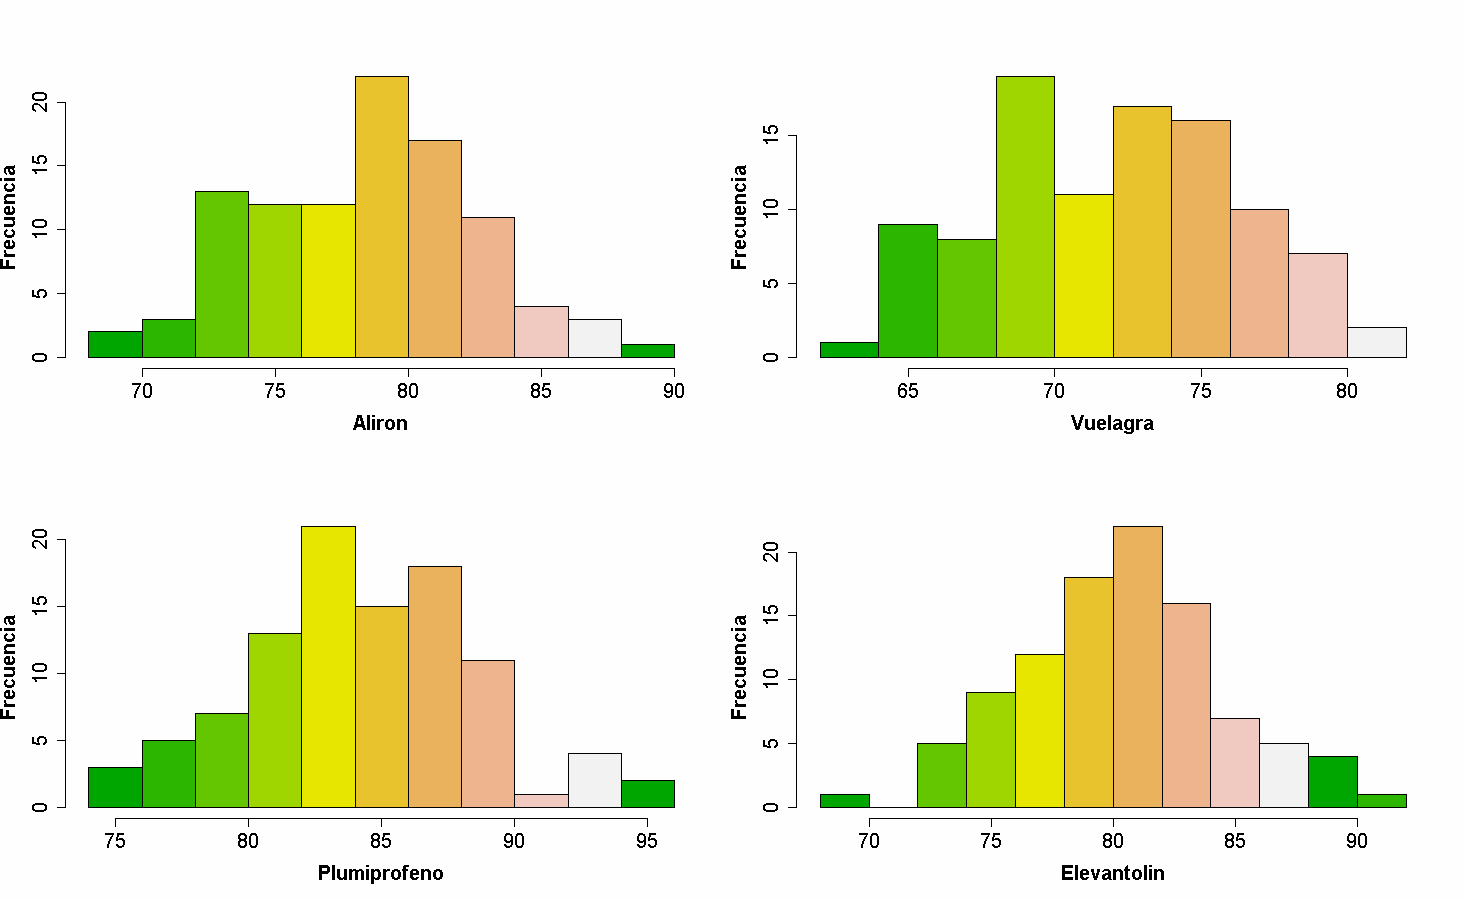
\includegraphics[width=14cm]{../fig/Cap11-HistogramasGrupos.png}\\[3mm]
(b)\\
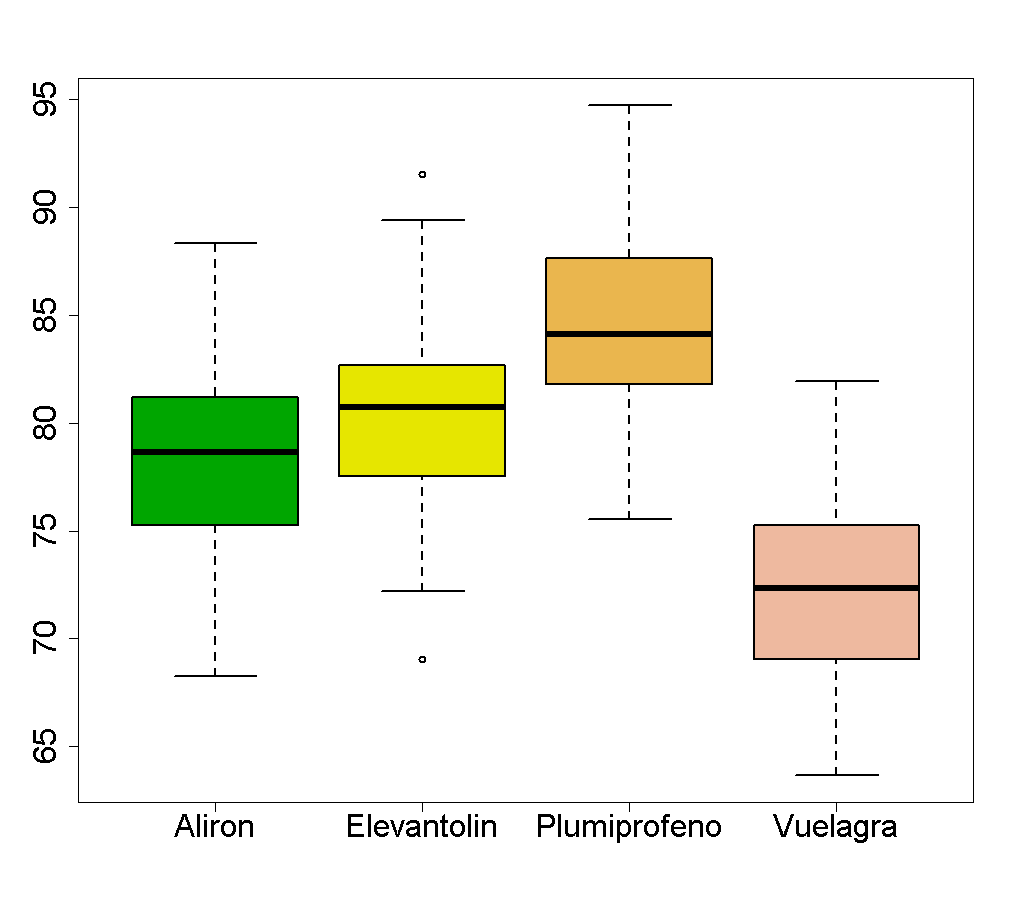
\includegraphics[width=9cm]{../fig/Cap11-BoxplotsParalelos.png}\\
\end{enColor}
\begin{bn}
(a)\\
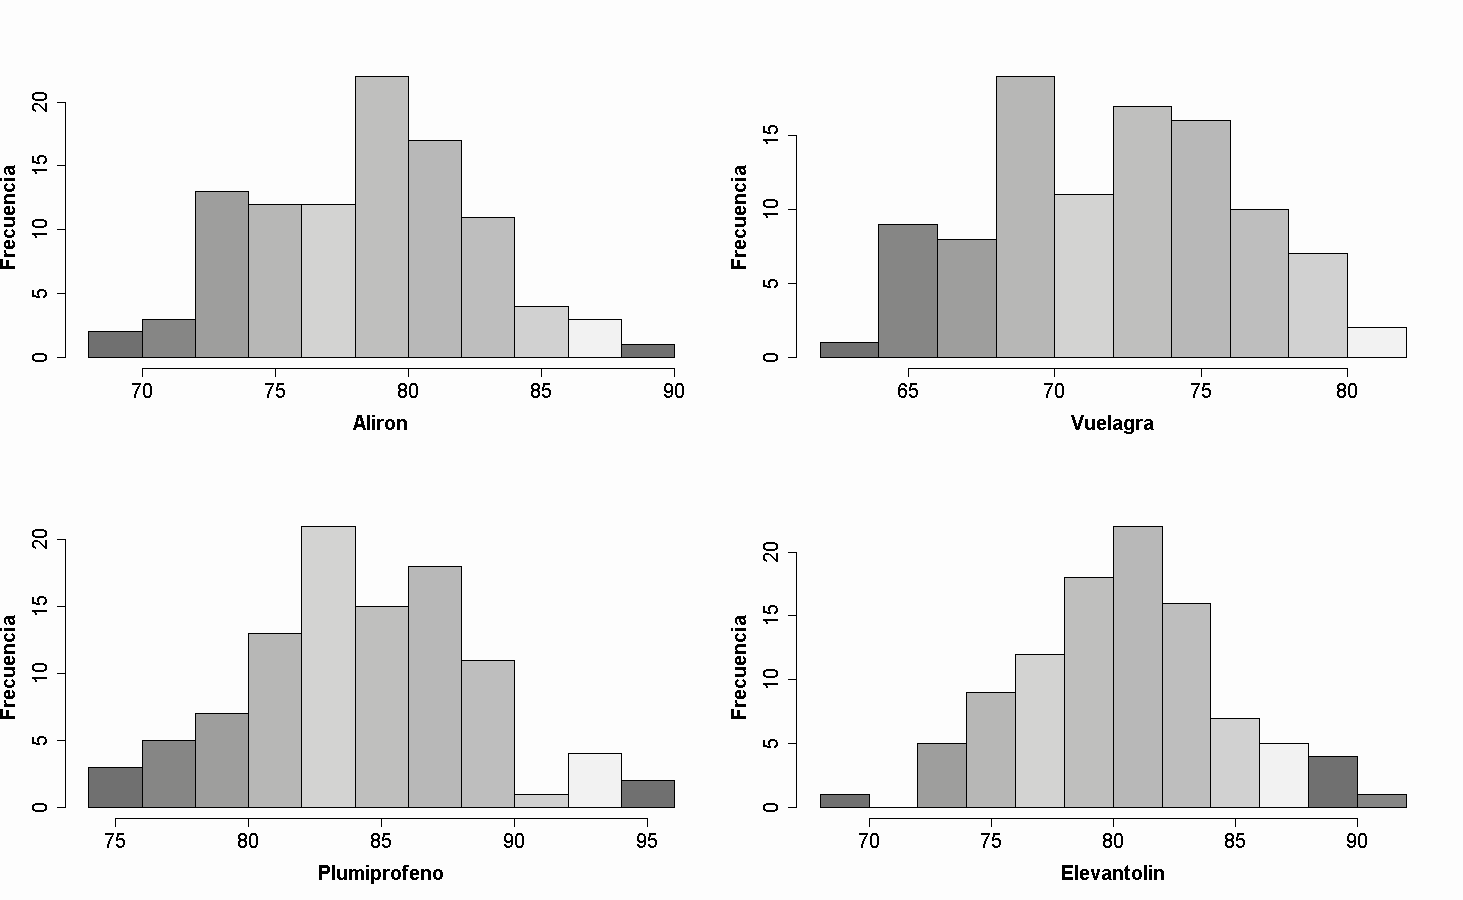
\includegraphics[width=14cm]{../fig/Cap11-HistogramasGrupos-bn.png}\\[3mm]
(b)\\
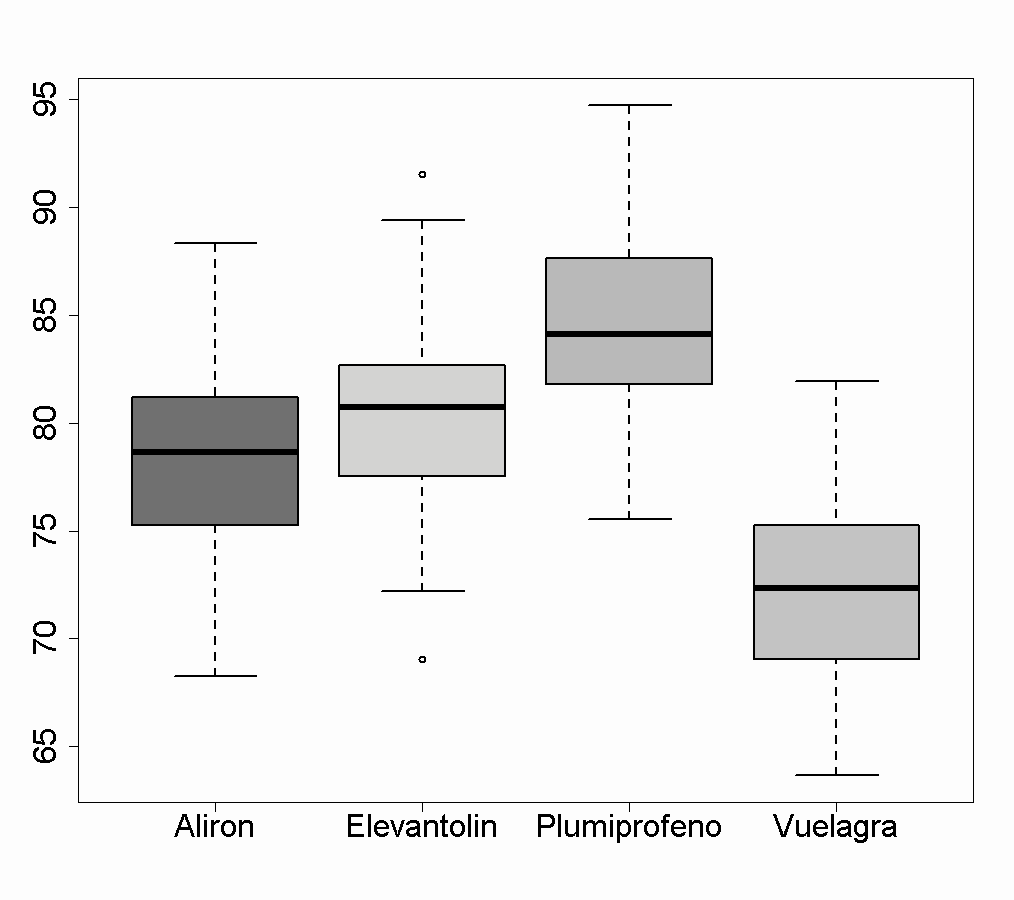
\includegraphics[width=9cm]{../fig/Cap11-BoxplotsParalelos-bn.png}\\
\end{bn}
\caption{(a) Histogramas y (b) diagramas de cajas paralelos para la condición de normalidad.}
\label{cap11:fig:BoxplotsParalelos}
\end{center}
\end{figure}

\begin{figure}[p]
\begin{center}
(c)\\
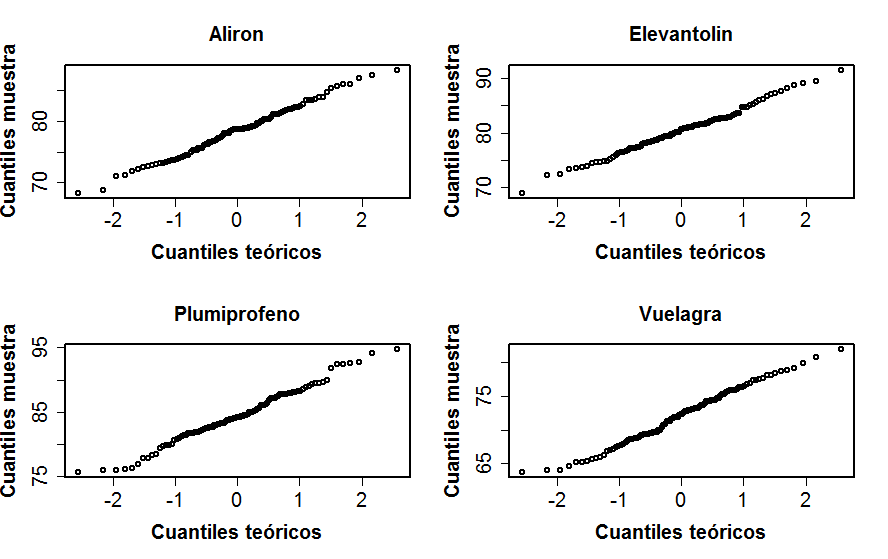
\includegraphics[width=14cm]{../fig/Cap11-EjemploFrailecillosQQplotsGrupos.png}\\[3mm]
(d)\\
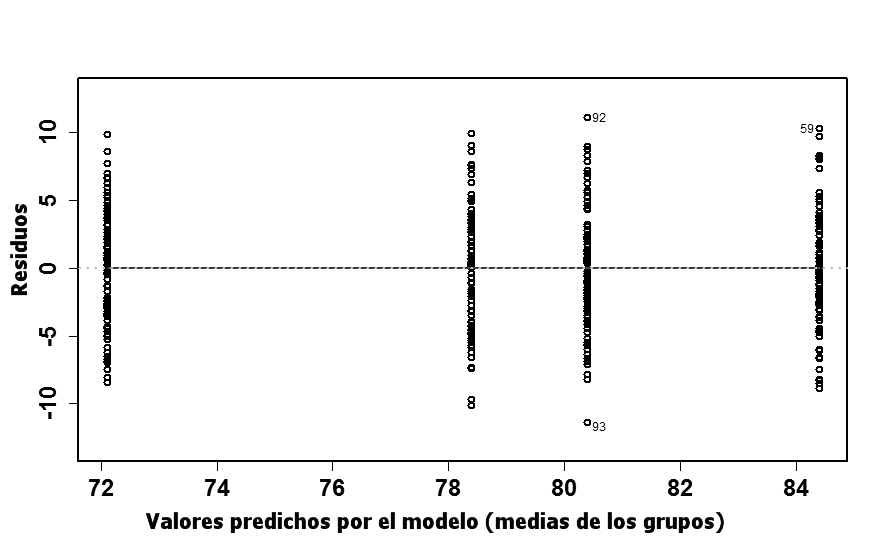
\includegraphics[width=13cm]{../fig/Cap11-EjemploFrailecillos-ResidualsVsFitted.png}\\
{\bf Figura \ref{cap11:fig:BoxplotsParalelos}, continuación. (c) QQ-plots por grupos (d) Residuos frente a valores predichos por el modelo.}
\end{center}
\end{figure}


\subsubsection{Comprobando la homogeneidad de las varianzas}
\label{cap11:subsubsec:ComprobandoHipotesisHomogeneidadVArianzasAnova}


La tercera condición, la de la homogeneidad de las varianzas de los distintos niveles del factor (homocedasticidad) es, a menudo, la más delicada y la que más quebraderos de cabeza nos puede causar. Si los grupos son todos del mismo tamaño (lo que hemos llamado un diseño equilibrado)\index{diseño
equilibrado},  ya hemos comentado que Anova es bastante robusto frente a diferencias no demasiado grandes en las varianzas. Pero con grupos de distinto tamaño, el método pierde potencia rápidamente ({\em potencia} en el sentido que hemos discutido en la Sección \ref{cap07:sec:PotenciaContraste} del Capítulo \ref{cap:ContrasteHipotesis}). ¿Cómo se puede verificar si se cumple esa homogeneidad de las varianzas?

Para empezar, debemos calcular las cuasivarianzas muestrales de cada uno de los grupos, y comprobar si existen grandes diferencias entre ellas. También podemos usar algunas de las herramientas gráficas que ya hemos usado para verificar la condición de normalidad.
\begin{ejemplo}
Los valores de las cuasidesviaciones típicas de los grupos del Ejemplo \ref{cap11:ejem:Anova01} de los frailecillos aparecen en la Tabla \ref{cap11:tabla:CuasidesviacionesPorGruposEjemploFrailecillos}. En este ejemplo, en el que hemos {\em ``cocinado''} los datos usando el ordenador, la homogeneidad de las varianzas se cumple más allá de lo que cabría esperar en un ejemplo real.
\begin{table}[ht]
\centering
\begin{tabular}{rrrr}
  \hline
 Aliron & Elevantolin & Plumiprofeno & Vuelagra \\
  \hline
 4.1996 & 4.1998 & 4.1999 & 4.1995 \\
   \hline
\end{tabular}
\caption{Cuasidesviaciones típicas de los grupos del Ejemplo \ref{cap11:ejem:Anova01}}
\label{cap11:tabla:CuasidesviacionesPorGruposEjemploFrailecillos}
\end{table}
En cuanto a las herramientas gráficas, los histogramas por grupos y los boxplots paralelos de la Figura \ref{cap11:fig:BoxplotsParalelos} (partes (a) y (b)) permiten cerciorarse, visualmente, de que la dispersión de todos los grupos es similar.
\qed
\end{ejemplo}

Aunque las herramientas anteriores son útiles, el análisis de la homogeneidad de las varianzas para Anova no estaría completo sin un examen de la distribución de los residuos, similar a la que hicimos en el caso del modelo de regresión lineal simple. Ya hemos visto (en la Ecuación \ref{cap11:ecu:AnovaIdentidadEstimadores}, pág. \pageref{cap11:ecu:AnovaIdentidadEstimadores} y en la discusión que la sigue) el significado de los residuos en el contexto de Anova.  Recuerda que el residuo correspondiente al valor muestral $x_{ij}$ era
\[(x_{ij}-\bar X_{\mbox{\bf\large $\cdot$}j}).\]
Sin entrar en otras posibilidades más formales, a menudo los residuos se analizan también gráficamente. Por ejemplo, usando un gráfico de los residuos frente a los valores que predice el modelo (ordenados por tamaño, claro. Recordemos que, en Anova, los valores predichos por el modelo son las medias de los grupos). Si en ese gráfico los puntos aparecen con forma de cuña (o con algún otro patrón claramente definido), podemos sospechar que hay una dependencia entre la media y la varianza. Por lo tanto, concluiremos que no se cumple la hipótesis de homogeneidad de varianzas.
\begin{ejemplo}
En la parte (d) de la Figura \ref{cap11:fig:BoxplotsParalelos} se muestran ese gráfico de residuos frente a frente a valores predichos para el Ejemplo \ref{cap11:ejem:Anova01}. Los valores predichos son las cuatro medias de cada uno de los niveles. Por esa razón vemos cuatro grupos de puntos, con cada grupo situado sobre el valor en el eje horizontal de cada una de las medias. Como puede verse, no existe en ese gráfico ningún patrón apreciable que parezca indicar que existe relación entre las medias y las varianzas de los grupos.
\qed
\end{ejemplo}

¿Qué sucede si no podemos verificar que se satisfacen las condiciones para aplicar Anova? Por ejemplo, si las muestras son pequeñas entocnes, como hemos dicho,  los métodos que se usan habitualmente para comprobar la normalidad son poco fiables. En ese caso, podemos recurrir a alguno de los llamados {\sf métodos no paramétricos}\index{métodos no paramétricos}, como el contraste de Kruskal-Wallis. Daremos alguna indicación adicional sobre estos métodos no paramétricos en el Apéndice \ref{apendice:MasAlla}.


\section{Anova significativo. Comparaciones por parejas.}
\label{cap11:sec:AnovaSignificativoComparacionesDosaDos}

Si el contraste Anova es significativo  (es decir, si el p-valor es bajo), concluiremos que hay evidencia estadística para rechazar la hipótesis nula. Por lo tanto, la conclusión es que las medias $\mu_i$ no son todas iguales.  Queremos precisar esto, porque a veces genera confusión. Si, por ejemplo, estamos trabajando en un problema en el que el factor tiene cinco niveles, y rechazamos la hipótesis nula de Anova, la conclusión {\em no es que las cinco medias son todas distintas unas de otras.} La conclusión correcta es que, {\em al menos, existen dos medias distintas, de entre esas cinco}. Pero puede ocurrir, por ejemplo, que sea $\mu_1=\mu_3=\mu_4$, mientras que $\mu_2$ y $\mu_5$ son distintas de esas tres medias, y también entre sí. Hay muchas situaciones distintas en las que la hipótesis nula $H_0$ resulta falsa, y sólo una forma de que sea verdadera, cuando todas las medias coinciden.

Por lo tanto, si hemos rechazado $H_0$ en Anova ({!`}y sólo en ese caso!), surge de manera natural la necesidad de saber qué medias (o grupos de medias) son (significativamente) distintas entre sí.

La primera idea que se nos ocurrirá, para resolver ese problema, es hacer {\sf comparaciones por parejas}\index{comparaciones por parejas, Anova unifactorial} (en inglés, {\em pairwise comparisons}\index{pairwise comparisons, one-way Anova}), comparando el grupo $i$ con el grupo $j$ para todas las posibles parejas con $i\neq j$. Se usa también el término en latín {\sf post-hoc}\index{post-hoc, comparaciones en Anova} (que podemos traducir por {\em después de}) para referirse a estas comparaciones, poniendo el énfasis en que son comparaciones que se hacen {\em después de} un resultado significativo del contraste Anova (e, insistimos, sólo en ese caso). En inglés se usa, asimismo, {\em post-hoc comparisons}.

¿Cuántas comparaciones son necesarias?
\begin{ejemplo}
\label{cap11:ejem:ComparacionesMultiples01}
Si tenemos una situación como la del Ejemplo \ref{cap11:ejem:Anova01}, en la que el factor tiene cuatro niveles, entonces las posibles comparaciones por parejas son:
\begin{enumerate}
  \item $\mu_1$ con $\mu_2$.
  \item $\mu_1$ con $\mu_3$.
  \item $\mu_1$ con $\mu_4$.
  \item $\mu_2$ con $\mu_3$.
  \item $\mu_3$ con $\mu_4$.
  \item $\mu_3$ con $\mu_4$.
\end{enumerate}
Y lo hemos escrito así para que tengas la oportunidad de pensar sobre la combinatoria que hay detrás de esta situación.
\end{ejemplo}
Estas comparaciones dos a dos se llaman también a veces {\sf comparaciones post-hoc}\index{post-hoc, comparaciones (en Anova unifactorial)}.

¿Cuántas comparaciones hay que hacer, si tenemos $k$ niveles del factor? Recordando la Combinatoria que aprendimos en el Capítulo \ref{cap:Probabilidad}, el número de parejas se calcula mediante el número combinatorio
    \[\binom{k}{2}=\dfrac{k(k-1)}{2}.\]
Así, para $k=4$ (como en el ejemplo anterior) hay que hacer $(4\cdot 3)/2=6$ comparaciones.

En principio, podríamos pensar en que cada una de esas comparaciones de dos medias se puede hacer con uno de los contrastes de comparación de dos medias, en poblaciones normales, que aprendimos en el Capítulo \ref{cap:Inferencia2Poblaciones}.  Pero hay dos observaciones importantes a tener en cuenta.

\begin{enumerate}
  \item Supongamos que decidimos trabajar a un nivel de significación $ns=1-\alpha$. Recordemos que $\alpha$ indica la probabilidad de cometer un error de tipo I, y por lo tanto, la probabilidad de afirmar que existe una diferencia entre las medias de dos grupos, cuando en realidad no es así. Si en cada una de las $\binom{k}{2}$ comparaciones necesarias corremos el riesgo de cometer un error de tipo I con una probabilidad del 5\%, entonces es fácil (ya que las comparaciones son independientes entre sí) ver que la probabilidad total de cometer ese error al menos una vez en la serie completa de comparaciones es bastante alta, incluso con un número relativamente pequeño de factores del nivel.
      \begin{ejemplo}
      Con un factor con $6$ niveles, y trabajando con $\alpha=0.05$, se tiene:
        \[P(\mbox{al menos un error de tipo I en 15 comparaciones})=1-P(\mbox{ningún error})=\]
        \[=1-(0.95)^{15}\approx 0.537\]
      Es decir, que tenemos una probabilidad mayor del 50\% de cometer un error de tipo I.\\
      Otra manera de llegar al mismo resultado es usando el hecho de que si pensamos en una variable aleatoria $Y$ cuyo valor es el número de errores de tipo I cometidos en la serie de $\binom{k}{2}=15$ comparaciones, entonces $Y$ es una binomial, con una probabilidad de éxito $\alpha$. Así que basta con calcular $P(Y\geq 1)$, usando la binomial.
      \qed
      \end{ejemplo}
     Con menos grupos el problema es menor, pero aún así grave. Y, por supuesto, a medida que aumenta el número de grupos, esta probabilidad aumenta hasta hacerse casi una certeza a partir de diez o más grupos. La conclusión evidente es que no podemos lanzarnos a hacer las comparaciones sin más.

  \item Cuando estudiamos los contrastes de igualdad de medias, en la Sección \ref{cap09:sec:diferenciaMediasDosPoblaciones} (pág. \pageref{cap09:sec:diferenciaMediasDosPoblaciones},; pero ver también los ejemplos de la Sección \ref{cap09:subsec:EjemplosContrasteDiferenciaMediasUsandoT}, pág. \pageref{cap09:subsec:EjemplosContrasteDiferenciaMediasUsandoT}), una de las peculiaridades de ese problema es que, en el caso de muestras pequeñas, teníamos que realizar un contraste previo de igualdad de las varianzas, para saber cuál era el estadístico adecuado. En principio podría parecer que ahora, al comparar cada pareja de medias, vamos a volver a encontrarnos con ese problema; al menos en el caso de muestras pequeñas. Pero, por otra parte, para rechazar la hipótesis nula hemos usado Anova, y hemos tenido que verificar que se cumplen las condiciones de ese método. Entre ellas ocupa un lugar destacado la homogeneidad de las varianzas entre distintos niveles del factor. Así que la propia utilización del método Anova, para ser correcta, obliga a trabajar con la hipótesis de que las varianzas de los distintos grupos son iguales. Eso implica, en primer lugar, que nos ahorramos ese trabajo. Pero es que, además, la estimación de ese valor de la varianza (que estamos suponiendo que es el misma para todos los grupos), puede hacerse entonces mediante la {\sf cuasidesviación típica ponderada} de las cuasidesviaciones típicas muestrales de las muestras de cada uno de los niveles. En el Capítulo \ref{cap:Inferencia2Poblaciones} hemos visto varios de estos ejemplos de cálculo de estimadores ponderados, para proporciones muestrales (en la Ecuación \ref{cap09:ecu:ProporcionMuestralPonderada}, pág. \pageref{cap09:ecu:ProporcionMuestralPonderada}), y para las cuasidesviaciones típicas muestrales, en el contraste de tipo (c) de la Sección \ref{cap09:sec:diferenciaMediasDosPoblaciones} (pág. \pageref{cap09:sec:diferenciaMediasDosPoblaciones}), que se puede considerar como el antecedente más claro de la situación que tenemos ahora aquí.
\end{enumerate}

Vamos a dar enseguida detalles que desarrollen estas dos observaciones. Pero antes, y para cerrar esta introducción al tema de las comparaciones  por parejas, queremos llamar la atención del lector sobre una particularidad de este problema. A lo largo de todo este capítulo nos hemos esforzado en mostrar los paralelismos entre el Anova unifactorial y el modelo de regresión lineal simple del Capítulo \ref{cap:RegresionLinealSimple}. Pero este tema de las comparaciones post-hoc, por parejas, es específico de Anova, y no tiene traducción sencilla al modelo de regresión.

\subsection{El ajuste de Bonferroni.}
\label{cap11:subsec:Bonferroni}

Uno de los remedios tradicionales al problema del control del error de tipo I en comparaciones múltiples es utilizar lo que se conoce como {\sf ajuste de Bonferroni}\index{ajuste de Bonferroni}. Aunque, como veremos, hay alternativas mejores, vamos a describirlo porque tiene la ventaja de la sencillez, y aporta una primera idea de lo que se busca y, a la vez, de lo que debemos evitar.

Con este método, el nivel de significación se reparte entre las distintas comparaciones que debemos realizar, de manera que se garantiza el control de la {\sf tasa global de errores}\index{tasa global de errores de tipo I} (en inglés, {\em family-wise (type I) error rate}\index{family-wise error rate}, abreviada a menudo en {\sf FWER}\index{FWER, family-wise error rate}). Es decir, se garantiza que la probabilidad de cometer un error de tipo I, en el conjunto completo de comparaciones dos a dos, se mantiene por debajo de $\alpha$.

El método parte de las comparaciones dos a dos, en las que, para contrastar si $\mu_i=\mu_j$, se usa el estadístico:
\begin{equation}
\label{cap11:ecu:EstadisticoComparacionesPostHoc}
\Upsilon=
\dfrac{\bar X_{{\mbox{\bf\large$\cdot$}}i}-\bar X_{{\mbox{\bf\large$\cdot$}}j}}{
{\sqrt{s_{\mbox{pond}}^2\cdot\left(\dfrac{1}{n_i}+\dfrac{1}{n_j}\right)}}},
\end{equation}
siendo $n_i, n_j$ y $\bar X_{{\mbox{\bf\large$\cdot$}}i}$, $\bar X_{{\mbox{\bf\large$\cdot$}}j}$ los tamaños y las medias muestrales, respectivamente,  de las muestras de esos dos niveles, y donde
\begin{equation}
\label{cap11:ecu:CuasivarianzaPonderadaComparacionesPostHoc}
s_{\mbox{pond}}^2=\dfrac{\sum_{i=1}^k (n_j-1)\cdot s_j^2}{N-k}=
\dfrac{\sum_{j=1}^k\sum_{i=1}^{n_j}(x_{ij}-\bar X_{\mbox{\bf\large $\cdot$}j})^2}{N-k}
=\dfrac{SS_{\mbox{\tiny residual}}}{N-k}
\end{equation}
es la {\sf cuasivarianza muestral ponderada}\index{cuasivarianza muestral ponderada, comparaciones por parejas} (en inglés, {\em pooled variance}\index{pooled variance, in pairwise comparisons}). Como se ve, $s_{\mbox{pond}}^2$ es uno de los ingredientes (el denominador, concretamente) del estadístico que usamos para el propio contraste Anova (ver la Ecuación \ref{cap11:ecu:distribucionMuestralAnova1Fequilibrado}, pág. \pageref{cap11:ecu:distribucionMuestralAnova1Fequilibrado}).  En la Ecuación \ref{cap11:ecu:EstadisticoComparacionesPostHoc} el símbolo
\[
s_j^2=\dfrac{\sum_{i=1}^{n_j}(x_{ij}-\bar X_{\mbox{\bf\large $\cdot$}j})^2}{n_j-1}
\]
representa la cuasivarianza muestral de la muestra del grupo (o nivel) número $j$ del factor. Fíjate en que en el cálculo de $s_{\mbox{pond}}^2$ intervienen todos los niveles, y no sólo los dos que se están comparando.

Para seguir adelante, necesitamos saber que el estadístico de la Ecuación \ref{cap11:ecu:EstadisticoComparacionesPostHoc} sigue una distribución $t$ de Student con $df=N-k$ grados de libertad.  Pero lo más importante del ajuste de Bonferroni es que, al calcular el p-valor, se hace el cálculo habitual en un contraste bilateral, pero {\em se multiplica ese valor por el número total de comparaciones}, que es, recordémoslo:
\[\binom{k}{2}.\]
Y a la vez, se controla que el valor así obtenido no supere $1$, claro. Por lo tanto, se tiene:\\

    \fcolorbox{black}{Gris025}{
        \begin{minipage}{12cm}
        \begin{center}
        {\bf Ajuste de Bonferroni}
        \index{Bonferroni, ajuste de}
        \end{center}
        Para aplicar el ajuste de Bonferroni, en cada una de las $\binom{k}{2}$ comparaciones entre niveles, el p-valor se calcula usando la fórmula:
        \begin{equation}
        \label{cap11:ecu:pValorAjusteBonferroni}
        \mbox{p-valor}=
        \min\left\{\mathbf{\binom{k}{2}}\cdot 2\cdot P\left(T_{N-k}>|\Upsilon|\right), 1\right\},
        \end{equation}
        siendo $\Upsilon$ el estadístico de la Ecuación \ref{cap11:ecu:EstadisticoComparacionesPostHoc}.
        \end{minipage}
    }\\[3mm]
La novedad, desde luego, es ese factor $\binom{k}{2}$ que hemos destacado (junto con el hecho de que  tomamos el mínimo para asegurarnos de que el p-valor en ningún caso es mayor que $1$).

\begin{ejemplo}
\label{cap11:ejem:BonferroniFrailecillos}
Para los datos del Ejemplo \ref{cap11:ejem:Anova01}, la cuasivarianza muestral ponderada es (usando los datos del Ejemplo \ref{cap11:ejem:Anova01e}, pág. \pageref{cap11:ejem:Anova01e}):
\[
s_{\mbox{pond}}^2=\dfrac{SS_{\mbox{\tiny residual}}}{N-k}=\dfrac{6984.41}{396}\approx 4.20
\]
Así que, para, por ejemplo, la diferencia entre { Alirón} y { Elevantolín} (datos muestrales en el Ejemplo \ref{cap11:ejem:FrailecillosCalculoMediasGrupos}, pág. \pageref{cap11:ejem:FrailecillosCalculoMediasGrupos}), se obtiene este estadístico:
\[\Upsilon=
\dfrac{\bar X_{{\mbox{\bf\large$\cdot$}}i}-\bar X_{{\mbox{\bf\large$\cdot$}}j}}{
{\sqrt{s_{\mbox{pond}}^2\cdot\left(\dfrac{1}{n_i}+\dfrac{1}{n_j}\right)}}}
\approx
\dfrac{78.40-72.10}{{\sqrt{4.20\cdot\left(\dfrac{1}{100}+\dfrac{1}{100}\right)}}}
\approx -3.368
\]
Y calculando el p-valor de acuerdo con la Ecuación \ref{cap11:ecu:pValorAjusteBonferroni} se obtiene:
\[
\mbox{p-valor}=
\min\left({\binom{4}{2}}\cdot 2\cdot P\left( T_{396}>|-3.368|\right), 1\right)
\approx 0.00499
\]
Por lo tanto, la diferencia entre { Alirón} y { Elevantolín} es significativa. El resto de las seis comparaciones por parejas también dan resultados significativos, con p-valores aún más pequeños. Para presentar los resultados de un conjunto de comparaciones emparejadas, podemos utilizar una tabla como la Tabla \ref{cap11:tabla:BonferroniFrailecillos}. Sólo se usa  la mitad inferior de la tabla, porque la mitad superior contiene las mismas parejas en el orden contrario. Como puede verse, los p-valores son todos extremadamente pequeños, así que, en este ejemplo, las medias de los cuatro niveles del factor son, en todos los casos, distintas dos a dos.


\begin{table}[ht]
\centering
\begin{tabular}{rccc}
  \hline
 & Aliron & Elevantolin & Plumiprofeno \\
  \hline
Elevantolin & $0.00499$ & * & * \\
  Plumiprofeno & $9.97\cdot 10^{-21}$ & $3.46\cdot 10^{-10}$ & * \\
  Vuelagra & $1.60\cdot 10^{-22}$ & $1.40\cdot 10^{-35}$ & $2.62\cdot 10^{-64}$ \\
   \hline
\end{tabular}
\caption{Comparaciones por parejas de los tratamientos del Ejemplo \ref{cap11:ejem:Anova01}, con ajuste de Bonferroni}
\label{cap11:tabla:BonferroniFrailecillos}
\end{table}

Si, además, tenemos en cuenta nuestros resultados previos (ver, por ejemplo los boxplots paralelos de la Figura \ref{cap11:fig:BoxplotsParalelos}, pág. \pageref{cap11:fig:BoxplotsParalelos}), podemos concluir el mejor tratamiento es { Plumiprofeno}, y que, de hecho, la ordenación de los tratamientos es:
\[
    \underbrace{\mu_3}_{\mbox{ Plumiprofeno}} >
    \underbrace{\mu_2}_{\mbox{ Elevantolín}} >
    \underbrace{\mu_1}_{\mbox{ Alirón}} >
    \underbrace{\mu_4}_{\mbox{ Vuelagra}.}
\]

\begin{figure}[h!]
\begin{center}
\begin{enColor}
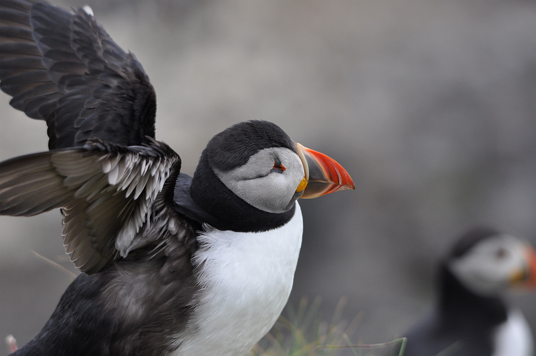
\includegraphics[width=6cm]{../fig/Cap11-Frailecillo.png}
\end{enColor}
\begin{bn}
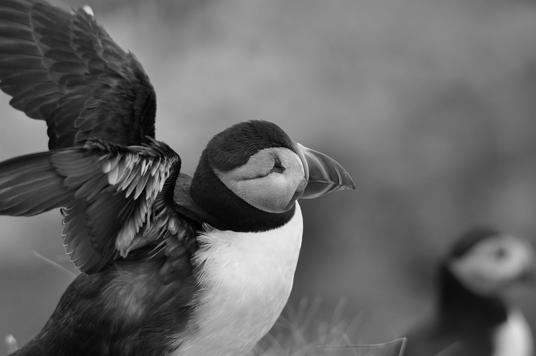
\includegraphics[width=6cm]{../fig/Cap11-Frailecillo-bn.png}
\end{bn}
\caption{El frailecillo, felizmente repuesto gracias a Anova.}
\label{cap11:fig:FrailecilloCurado}
\end{center}
\end{figure}
Queremos cerrar este ejemplo lanzando al lector una pregunta para que reflexione. Si hacemos una comparación entre parejas y concluimos que:
\[\mbox{ Plumiprofeno} > \mbox{ Elevantolín} \]
y después hacemos otra y concluimos que:
\[\mbox{ Elevantolín} > \mbox{ Alirón},\]
¿es realmente necesario hacer después la comprobación
\[\mbox{ Plumiprofeno} > \mbox{ Alirón}?\]
\qed
\end{ejemplo}

En el Tutorial11 aprenderemos a aplicar este ajuste de Bonferroni con el ordenador. Vamos a ver
otro ejemplo brevemente (ahorrándonos la comprobación de las condiciones del modelo Anova), en el que las medias de los niveles no son todas significativamente
diferentes, para ilustrar algunas peculiaridades de esa situación.

\begin{ejemplo}
\label{cap11:ejem:BonferroniMediasNoTodasDistintas}

El fichero adjunto
\begin{center}
\fichero{../datos/Cap11-ComparacionesPostHoc.csv}{\sf Cap11-ComparacionesPostHoc.csv}
\end{center}
contiene una tabla de datos (son {\em datos limpios}, en el sentido que se discute en el
Tutorial11), con $N=140$ valores de una variable continua llamada {\tt respuesta}, correspondientes
a seis niveles diferentes de un factor llamado {\tt tratamiento} (los seis niveles se llaman {\tt
grupo1, grupo2,} etc.) La Tabla \ref{cap11:tabla:BonferroniMediasNoTodasDistintasFicheroDatos}
muestra el comienzo de ese conjunto de datos.

\begin{table}[ht]
\begin{verbatim}
                    tratamiento respuesta
                103      grupo5     14.84
                104      grupo5     21.63
                82       grupo4     11.10
                129      grupo6     19.30
                10       grupo1     11.38
                120      grupo6     17.92
\end{verbatim}
\caption{Comienzo del fichero {\sf Cap11-ComparacionesPostHoc.csv}
 para el Ejemplo \ref{cap11:ejem:BonferroniMediasNoTodasDistintas}}
\label{cap11:tabla:BonferroniMediasNoTodasDistintasFicheroDatos}
\end{table}

A diferencia del otro Ejemplo que hemos visto en este capítulo, aquí los grupos no son todos del
mismo tamaño. En concreto se tiene:
\[
n_1=19, \quad n_2=29,\quad  n_3=26,\quad n_4=26,\quad n_5=15,\quad n_6=25,
\]
para un total de $N=n_1+\cdots+n_6=140$ observaciones. Así que se trata de un {\em diseño no
equilibrado}. En el Tutorial11 veremos la forma de hacer paso a paso el contraste Anova para estos datos. Allí daremos los detalles de cómo se debe verificar la hipótesis de normalidad y homogeneidad de varianzas. Pero, en este caso, al tratarse de datos que hemos preparado nosotros, sabemos {\em a priori}, que proceden de poblaciones normales con la misma varianza. Así que podemos hacer el contraste Anova de la hipótesis nula
\[H_0=\{\mu_1=\mu_2=\dots=\mu_6\}\]
y, como veremos en el Tutorial11, rechazaremos $H_0$, con un p-valor extremadamente pequeño
($<10^{-15}$).

Podemos, entonces, pasar a las comparaciones dos a dos de las medias de los grupos, y vamos a usar
el ajuste de Bonferroni. En este caso el número de factores es $k=6$, así que hay que hacer
\[\binom{6}{2}=15\]
comparaciones en total. La Tabla \ref{cap11:tabla:pValoresBonferroniMediasNoTodasDistintas} resume
los p-valores obtenidos (ya ajustados).

\begin{table}[ht]
\centering
\begin{tabular}{|r|c|c|c|c|c|}
    \hline
 & grupo1 & grupo2 & grupo3 & grupo4 & grupo5 \\
    \hline
\rule{0mm}{5mm}grupo2 & $1.1\cdot 10^{-15}$ & * & * & * & * \\
    \hline
  \rule{0mm}{5mm}grupo3 & $1$ & $3.5\cdot 10^{-14} $& * & * & * \\
    \hline
  \rule{0mm}{5mm}grupo4 & $0.1268$ & $1.4\cdot 10^{-10}$ & $1$& * &  *\\
    \hline
  \rule{0mm}{5mm}grupo5 & $1.6\cdot 10^{-9} $&$ 1$&$ 8.6\cdot 10^{-8}$ & $2.9\cdot 10^{-5}$ & * \\
    \hline
  \rule{0mm}{5mm}grupo6 & $0.0017$ & $3.9\cdot 10^{-7}$ & $0.0692$ & $1$& $0.0046$ \\
   \hline
\end{tabular}
\caption{Comparaciones por parejas de los tratamientos del Ejemplo \ref{cap11:ejem:BonferroniMediasNoTodasDistintas}, con ajuste de Bonferroni}
\label{cap11:tabla:pValoresBonferroniMediasNoTodasDistintas}
\end{table}
Como se ve, hay contrastes muy significativos, con p-valores muy pequeños, que indican que las
medias de esos grupos son, con seguridad, distintas. Pero también hay contrastes no significativos,
algunos incluso con un p-valor tan grande que el ordenador lo considera (al redondearlo) como igual a $1$.
\qed
\end{ejemplo}

Ahora que hemos visto un par de ejemplos de comparaciones múltiples, queremos llamar la atención del lector sobre algo que puede desconcertar a quienes se inician en este tema, porque es {\em aparentemente paradójico}. \\

    \fcolorbox{black}{Gris025}{
        \begin{minipage}{12cm}
        \begin{center}
        {\bf Anova significativo sin diferencias significativas por parejas}
        \end{center}
        Puede ocurrir que el resultado del contraste Anova nos lleve a rechazar la igualdad de las medias (en conjunto), pero que, al realizar las comparaciones por parejas seamos incapaces de detectar diferencias significativas entre ninguna de las parejas.
        \end{minipage}
    }\\[3mm]

Esto no significa que hayamos hecho nada mal al realizar el contraste Anova. Hay que tener en cuenta que Anova examina el conjunto de datos completo, mientras que las comparaciones por parejas tratan de responder a una pregunta específica sobre esa pareja. Quizá esta otra manera de verlo arroje algo más de luz, a la vez que nos recuerda el tema central de esta parte del curso: en el contexto de una relación de tipo $C \sim F$, el contraste Anova trata de responder a la pregunta ``¿hay una relación significativa entre la variable respuesta $X$ y los valores del (factor) tratamiento $T$?'' Pero incluso cuando la respuesta a esa pregunta es afirmativa, puede que seamos incapaces de encontrar diferencias significativas entre las respuestas medias para dos valores concretos de $T$. Es decir, sabemos que $X$ depende de $T$, pero no disponemos de datos que nos permitan describir con más detalle esa dependencia.

\begin{ejemplo}
\label{cap11:ejem:AnovaSignificativoPostHocNoSignificativo}
El fichero adjunto
\begin{center}
\fichero{../datos/Cap11-AnovaSignificativoPostHocNoSignificativo.csv}{Cap11-AnovaSignificativoPostHocNoSignificativo.csv}
\end{center}
contiene una tabla de datos ({\em limpios}), con $N=250$ valores de una variable continua llamada {\tt respuesta}, correspondientes a seis niveles diferentes de un factor llamado {\tt tratamiento} (los seis niveles se llaman {\tt grupo1, grupo2,} etc.) Las cinco muestras proceden de poblaciones normales, todas con la misma varianza, y constan de $50$ observaciones cada una. Al realizar el contraste Anova se obtiene un p-valor aproximadamente igual a $0.03134$. Así que, con un nivel de significación del $95\%$, podemos rechazar la hipótesis nula y concluir que hay diferencias significativas entre las medias.

Pero si realizamos las comparaciones post-hoc con el ajuste de Bonferroni, se obtiene la Tabla \ref{cap11:tabla:AnovaSignificativoPostHocNoSignificativo}, que muestra que, a ese nivel de significación, no podemos detectar diferencias significativas entre ningún par de medias concreto.

\begin{table}[ht]
\centering
\begin{tabular}{|r|c|c|c|c|}
  \hline
 & grupo1 & grupo2 & grupo3 & grupo4 \\
  \hline
  grupo2 & 1 & * & * & * \\
  \hline
  grupo3 & 0.06 & 1 & * &*  \\
  \hline
  grupo4 & 1 & 1 & 1 &  *\\
  \hline
  grupo5 & 1 & 1 & 0.06 & 1 \\
   \hline
\end{tabular}
\caption{Comparaciones por parejas de los tratamientos del Ejemplo \ref{cap11:ejem:AnovaSignificativoPostHocNoSignificativo}, con ajuste de Bonferroni}
\label{cap11:tabla:AnovaSignificativoPostHocNoSignificativo}
\end{table}

\qed
\end{ejemplo}


\subsubsection{Representaciones gráficas y ordenación de las medias}
\label{cap11:subsubsec:RepresentacionesGraficasOrdenacionMedias}


Supongamos ahora que el contraste Anova ha resultado significativo, y que en las comparaciones post-hoc también hemos detectado diferencias significativas entre pares concretos de medias. Una pregunta natural es ``¿cuál es la media más grande?'' (o la más pequeña). Desde un punto de vista más general, nos planteamos el problema de ordenar las medias por tamaño, como hicimos en el Ejemplo \ref{cap11:ejem:BonferroniFrailecillos} (pág. \pageref{cap11:ejem:BonferroniFrailecillos}), para los tratamientos de los frailecillos. Enseguida vamos a ver que las cosas no son tan sencillas como podría parecer a partir de la descripción un tanto ingenua de la situación que vimos en aquel ejemplo.

Un problema estrechamente relacionado con este es el de la representación gráfica adecuada para los datos en una situación como esta. El siguiente ejemplo trata de ilustrar estos dos problemas, con los datos del Ejemplo \ref{cap11:ejem:BonferroniMediasNoTodasDistintas}.

\begin{ejemplo}{\bf (Continuación del Ejemplo \ref{cap11:ejem:BonferroniMediasNoTodasDistintas})}
\label{cap11:ejem:BonferroniMediasNoTodasDistintas02}
La Tabla \ref{cap11:tabla:pValoresBonferroniMediasNoTodasDistintas} no parece la forma más adecuada
de resumir la información que hemos obtenido. Mirando esa tabla, no resulta evidente, a simple vista, qué medias son distintas y cuáles no. Por esa razón se suelen utilizar otro tipo de representaciones que hagan más evidentes esas diferencias. Una posibilidad es usar una representación gráfica como la de la Figura
\ref{cap11:fig:BonferroniMediasNoTodasDistintasBoxplotsGrupos}. En esa figura se muestran los
diagramas de caja de cada uno de los grupos. Pero lo más interesante, desde el punto de vista de
nuestra discusión actual, son las letras {\tt a, b, c} que aparecen en la parte superior de la
figura.

\begin{figure}[htbp]
\begin{center}
\begin{enColor}
\hrule
\quad\\[2mm]
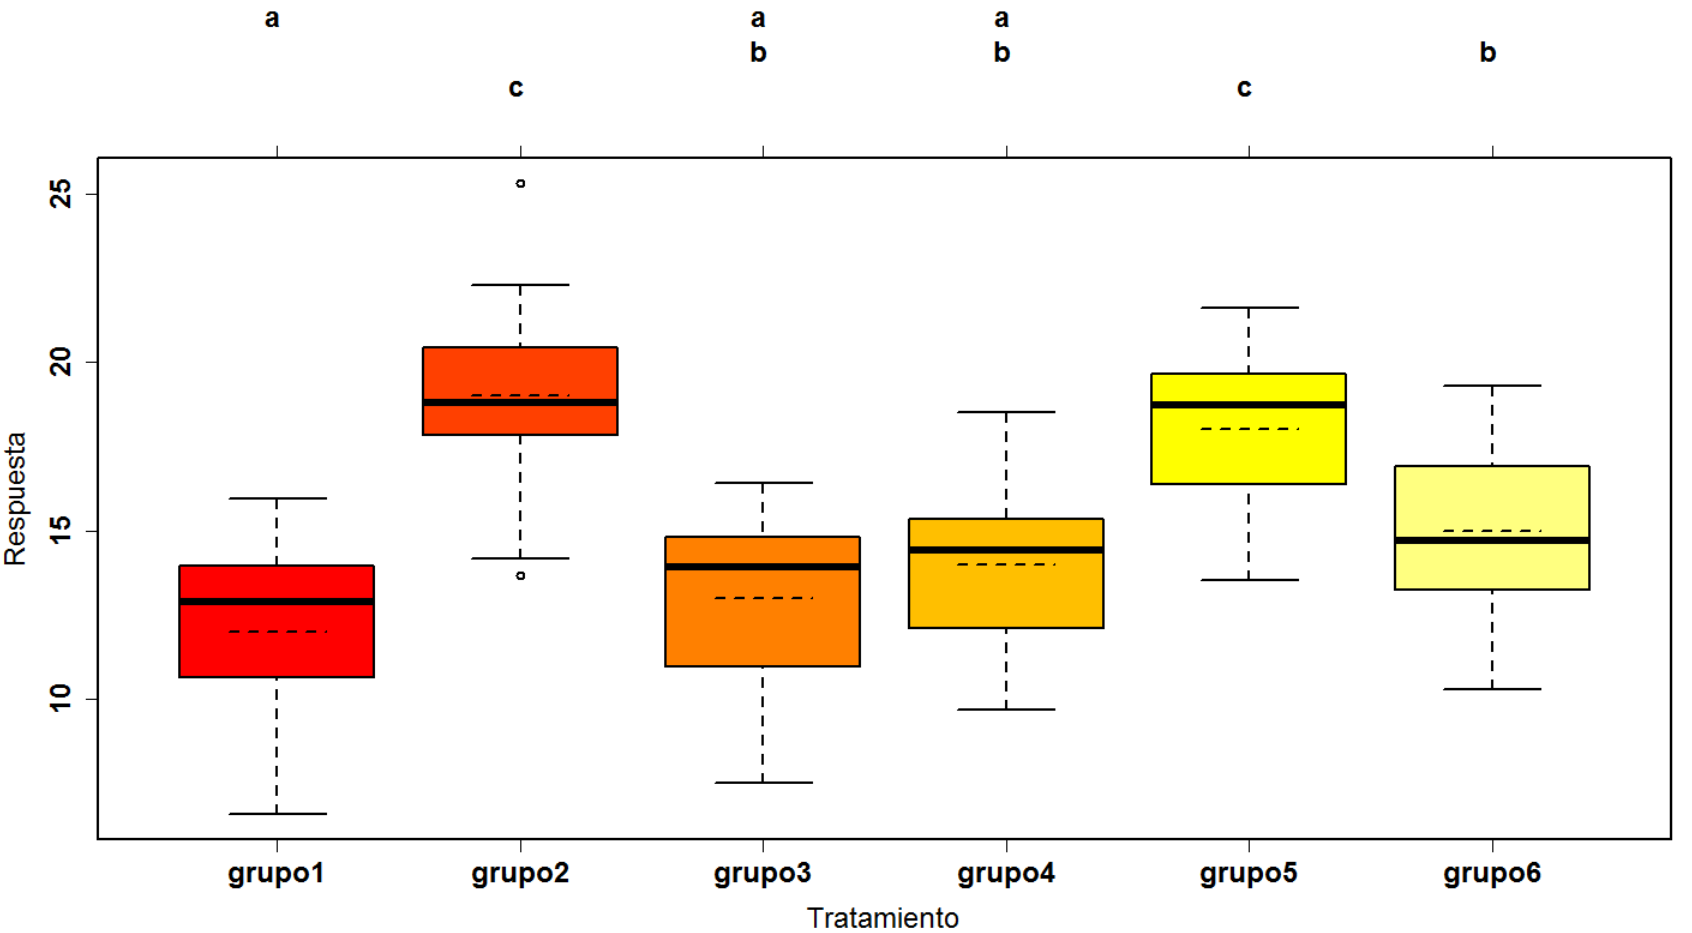
\includegraphics[width=13.5cm]{../fig/Cap11-BonferroniMediasNoTodasDistintas.png}

\hrule
\end{enColor}
\begin{bn}
\hrule
\quad\\[2mm]
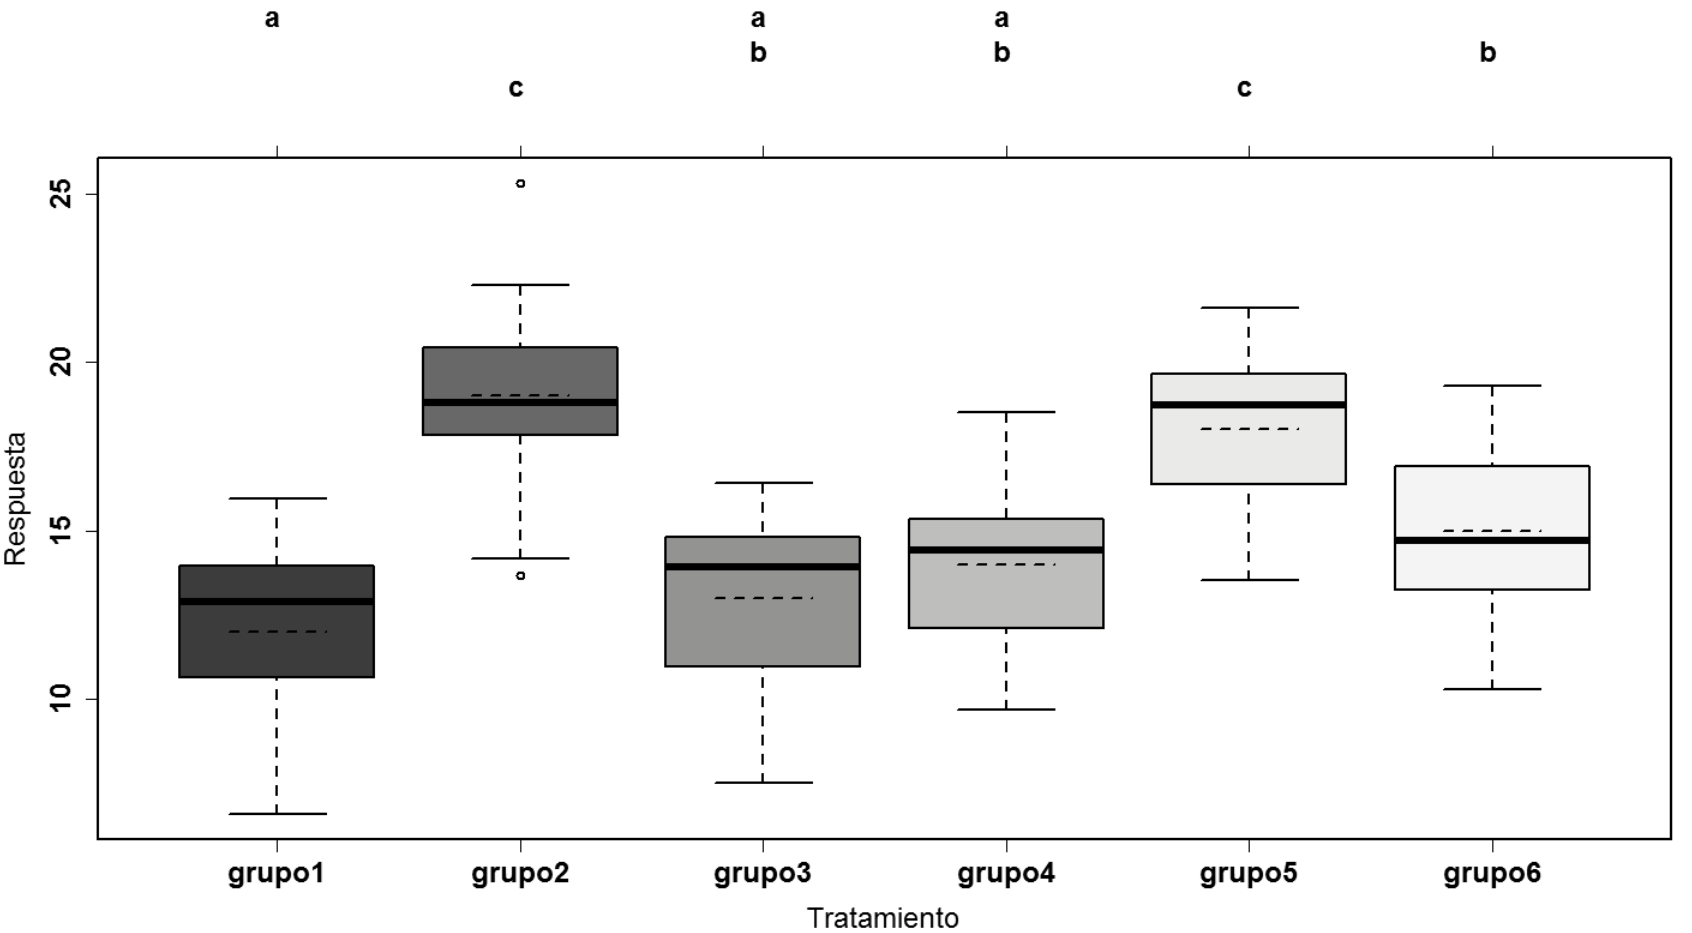
\includegraphics[width=13.5cm]{../fig/Cap11-BonferroniMediasNoTodasDistintas-bn.png}

\hrule
\end{bn}
\caption{Comparaciones por parejas de las medias del Ejemplo \ref{cap11:ejem:BonferroniMediasNoTodasDistintas}. Los segmentos horizontales discontinuos indican la altura a la que se sitúan las medias de cada grupo.}
\label{cap11:fig:BonferroniMediasNoTodasDistintasBoxplotsGrupos}
\end{center}
\end{figure}

Esas letras sirven para identificar los grupos cuyas medias no han resultado significativamente
distintas en el contraste. Por ejemplo, los grupos $1$, $3$ y $4$ aparecen rotulados con la letra
{\tt a}, y eso indica que las medias de esos tres grupos no son significativamente distintas. Lo
mismo sucede con los grupos $3$, $4$ y $6$ (letra {\tt b}) por un lado, y con los grupos $2$ y $5$
por otro (letra {\tt c}). El resumen es que si dos grupos comparten una de las letras {\tt a, b, c}, entonces sus medias no son significativamente distintas.
%Además, la altura a la que se sitúa la
%letra también nos indica si las medias de esos grupos son mayores que la de los grupos que
%corresponden a otra letra.
Pero cuidado. Si examinas la situación atentamente te darás cuenta de que la discusión es sutil.
Por ejemplo, sabemos que la media del grupo $1$ es significativamente distinta de la del grupo $6$,
porque no comparten ninguna letra. Pero, por otro lado,
\begin{itemize}
  \item no somos capaces de distinguir entre el grupo $1$ de los grupos $2$ y $3$,
  \item y no somos capaces de distinguir entre el grupo $6$ de los grupos $2$ y $3$.
\end{itemize}
Conviene que reflexiones un momento sobre esto, usando la Figura
\ref{cap11:fig:BonferroniMediasNoTodasDistintasBoxplotsGrupos} para acompañar la reflexión.
La conclusión de esas reflexiones es que la ordenación por tamaños de las medias que hemos obtenido
es lo que los matemáticos llaman una {\sf relación de orden parcial}\index{orden parcial, relación
de}\index{relación de orden parcial}, que se caracteriza porque no podemos contestar a todas las
preguntas de la forma
\[\mbox{¿es $a > b$?}\]
Sólo sabemos la respuesta en algunos casos. Esa relación se ilustra, para este ejemplo, en la
Figura \ref{cap11:fig:BonferroniMediasNoTodasDistintasRelacionOrdenParcial}. En esa figura, sólo
podemos decir que la media del grupo $i$ es significativamente mayor que la del grupo $j$ si existe
un camino de flechas que va desde la casilla $i$ a la casilla $j$.

\begin{figure}[htbp]
\begin{center}
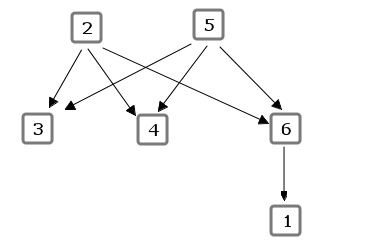
\includegraphics[width=8cm]{../fig/Cap11-BonferroniMediasNoTodasDistintasRelacionOrdenParcial.png}
\caption{Relación de orden parcial entre las medias del Ejemplo \ref{cap11:ejem:BonferroniMediasNoTodasDistintas}.}
\label{cap11:fig:BonferroniMediasNoTodasDistintasRelacionOrdenParcial}
\end{center}
\end{figure}

Como ves, el tema de los contrastes por parejas tiene más estructura de la que parece a primera vista.

También puede resultarte útil conocer otro tipo de representaciones gráficas, como la de la Figura
\ref{cap11:fig:BonferroniMediasNoTodasDistintasIntervalosGrupos} (basada en la Figura 7.1, pág. 135
del libro \cite{dalgaard2008introductory}, de Dalgaard). En esa figura los segmentos verticales
representan intervalos de confianza centrados en las respectivas medias muestrales de los grupos (que son el punto central destacado en cada uno de los segmentos). Las líneas que conectan los centros sirven sólo para ayudar a
situar las medias.

\begin{figure}[htbp]
\begin{center}
\begin{enColor}
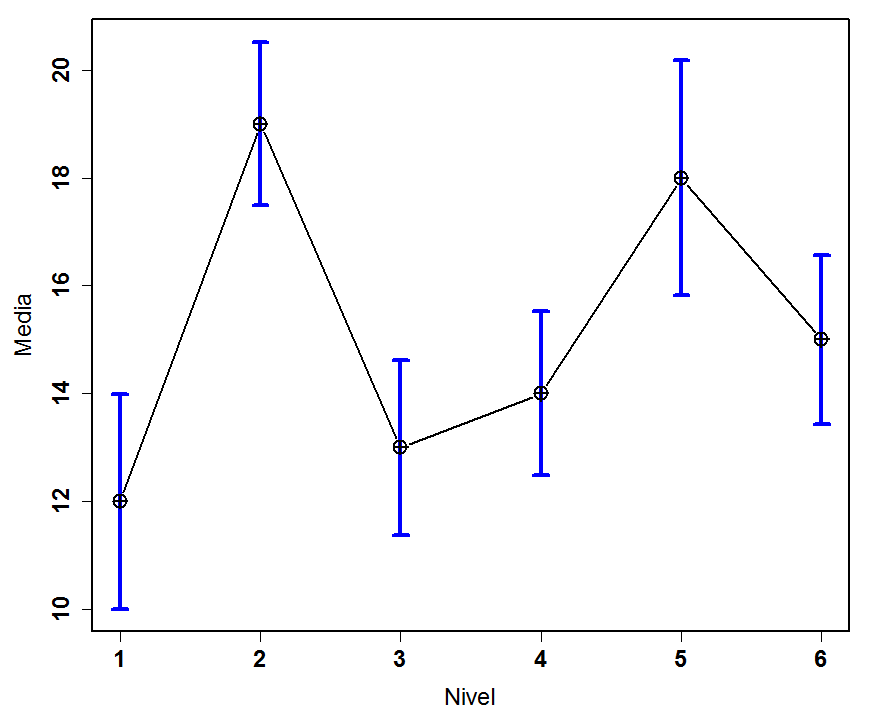
\includegraphics[width=10cm]{../fig/Cap11-BonferroniMediasNoTodasDistintasIntervalosConfianza.png}
\end{enColor}
\begin{bn}
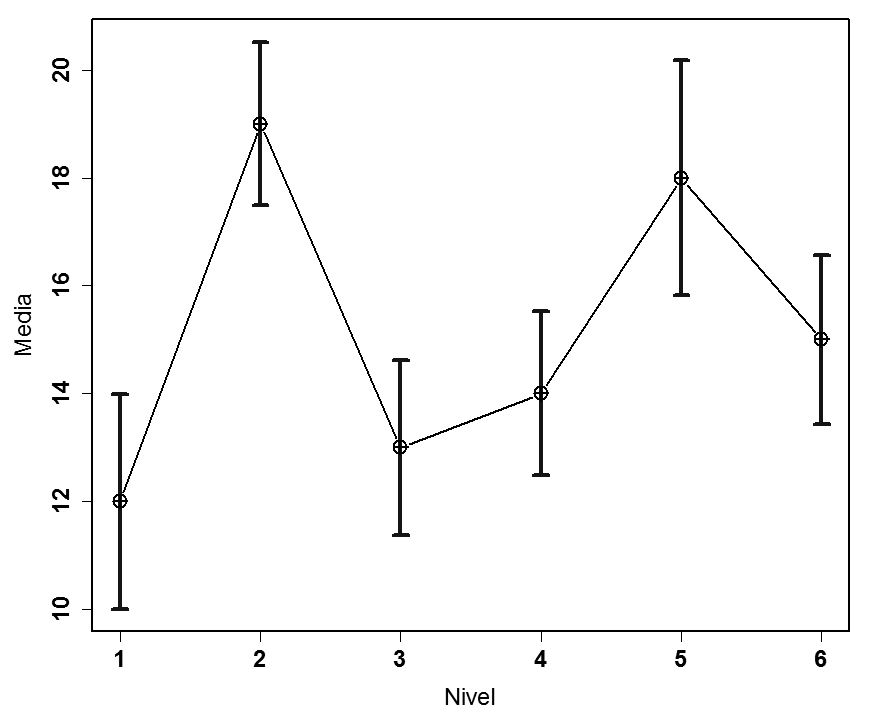
\includegraphics[width=10cm]{../fig/Cap11-BonferroniMediasNoTodasDistintasIntervalosConfianza-bn.png}
\end{bn}
\caption{Intervalos de confianza (ajustados por Bonferroni) para las medias del Ejemplo \ref{cap11:ejem:BonferroniMediasNoTodasDistintas}.}
\label{cap11:fig:BonferroniMediasNoTodasDistintasIntervalosGrupos}
\end{center}
\end{figure}

Los intervalos de confianza se han calculado con un nivel de confianza que usa el ajuste de
Bonferroni. Es decir, que para $k$ niveles, si queremos un nivel de confianza con $\alpha=0.05$
{\em en conjunto}, entonces cada intervalo se ha calculado usando
\[\hat\alpha=\dfrac{\alpha}{\binom{k}{2}},\]
que, en este ejemplo, es $\hat\alpha=\frac{0.05}{15}\approx 0.0033$. Como se ve, usamos un nivel de
confianza bastante más alto en cada intervalo individual. A pesar de que es posible hacerlo, no recomendamos que el lector se acostumbre a extraer conclusiones, en términos de inferencia, a partir de una figura como la \ref{cap11:fig:BonferroniMediasNoTodasDistintasIntervalosGrupos}.
%Con eso podemos asegurar que si dos intervalos de la Figura \ref{cap11:fig:BonferroniMediasNoTodasDistintasIntervalosGrupos} no solapan, entonces las medias correspondientes son significativamente diferentes.
\qed
\end{ejemplo}

Sin duda, una de las lecciones más importantes que queremos extraer de este ejemplo es algo que ya vimos en la Sección \ref{cap09:subsec:IntervalosDeConfianzaVsContrastes01} (pág. \pageref{cap09:subsec:IntervalosDeConfianzaVsContrastes01}), al contrastar la diferencia entre dos medias. En general no es una buena idea  tratar de usar intervalos de confianza para hacer el trabajo de un contraste de hipótesis de igualdad de medias. Y las cosas son aún peores si, en lugar de los intervalos de confianza se usan otro tipo de intervalos.
%Se trata de que la recíproca es falsa: {\bf aunque los intervalos solapen, puede que la conclusión correcta sea rechazar $H_0$ y concluir que esas medias son significativamente distintas.} Esto es una observación general sobre el uso de intervalos de confianza centrados en cada una de las medias, como forma de contrastar la diferencia entre ellas: no es, en general, una buena idea. Y sin embargo, este tipo de representaciones gráficas se usan  constantemente en las publicaciones científicas. Insistimos en que, cuando se utilizan intervalos de confianza para la representación gráfica, sólo se permiten las conclusiones en un sentido: las medias que parecen distintas son, de hecho, significativamente distintas. Pero las que parecen solapar, puede que hayan producido un p-valor significativo en el contraste.
Lamentablemente, como ya vimos en el caso de dos medias, son frecuentes las representaciones gráficas con {\em barras de error estándar}\index{barras de error estándar} (ver la Figura \ref{cap09:fig:GraficoBarrasError}, pág. \pageref{cap09:fig:GraficoBarrasError}), que aumentan la confusión sobre las  conclusiones en términos de inferencia que se pueden obtener cuando observamos un gráfico (si es que hay alguna). La mejor recomendación que podemos dar al lector es que no se fíe de recetas sencillas, cuando quiera estar seguro de la significación  estadística y la relevancia científica de un resultado. Internet está lleno de esas recetas (que en inglés se denominan {\em rules of thumb}), pero no hay mejor receta que la prudencia bien informada.

\subsubsection{Otros métodos para las comparaciones múltiples}

El problema con el ajuste de Bonferroni es que es demasiado {\em conservador}, en el sentido de que va demasiado lejos tratando de evitar los errores de tipo I. Y como ya discutimos en su momento, tratar de reducir la probabilidad de cometer un error de tipo I, lleva aparejado un aumento de la probabilidad de cometer errores de tipo II. Eso significa que, utilizando ese método, es más difícil que rechacemos la hipótesis nula cuando es falsa, y así dejaríamos de detectar una diferencia realmente significativa entre un determinado par de medias. Es decir, que el ajuste de Bonferroni se traduce en una importante pérdida de {\em potencia} (en el sentido de potencia que aparece en la Sección \ref{cap07:sec:PotenciaContraste}, pág. \pageref{cap07:sec:PotenciaContraste}).

Para paliar ese problema, los estadísticos han diseñado bastantes métodos con el objetivo de comparar las medias de los distintos grupos. Muchos de estos métodos se caracterizan, a menudo, por estar diseñados con un tipo específico de comparación de medias en mente. Daremos más detalles sobre este enfoque en el siguiente apartado. Otros métodos, en cambio, se parecen al de Bonferroni, en el sentido de que son adecuados cuando no tenemos razones para fijarnos en algun caso concreto, y simplemente queremos comparar todas las medias, en lo que se denomina {\sf comparaciones no planificadas}\index{comparaciones no planificadas, Anova} (en inglés, {\em unplanned comparisons}\index{unplanned comparisons, Anova}). El más conocido de estos métodos genéricos, como alternativa al de Bonferroni, es el {\sf método de Tukey}\index{método de Tukey}\index{Tukey, método}, (en inglés {\em Tukey's Honestly Significant Difference}, o {\em Tukey's HSD}). El lector encontrará más información en las referencias que aparecen en el Apéndice \ref{apendice:MasAlla}.

%Por ejemplo, uno de esos métodos, el contraste de Dunnett, se utiliza en aquellas situaciones en que, desde el principio, se dispone de un {\em grupo de control}, y lo que se desea es comparar la media de los demás grupos con la del grupo de control; no nos interesa comparar todos con todos, sino medir las posibles diferencias con el control. Y hay otros tipos de contrastes (SNK, Ryan, Duncan, Tukey, Scheffe, Peritz...), cada uno con su finalidad, sus pros y sus contras, que los hacen más adecuados (o populares) en distintos campos de trabajo (medicina, ecología, etc.)

\subsection{Introducción a los contrastes.}
\label{cap11:subsubsec:IntroduccionContrastes}

\noindent{\bf Opcional: esta sección depende de los resultados de la Sección \ref{cap11:subsec:AnovaComoModeloLineal}, pág. \pageref{cap11:subsec:AnovaComoModeloLineal}.}\\
\noindent{\bf Atención: la palabra {\em ``contraste''} en el título de esta sección tiene un significado especial, que se aclarará más adelante.}

Aunque esta parte del curso trata de la relación entre dos variables, al escribir la Ecuación
\ref{cap11:ecu:AnovaComoModeloLineal} (pág. \pageref{cap11:ecu:AnovaComoModeloLineal}; la reproducimos aquí por comodidad):
    \begin{equation}
    \label{cap11:ecu:AnovaComoModeloLinealRepetida}
        X=\beta_0+\beta_1\cdot T^{(1)}+\beta_2\cdot T^{(2)}+\cdots+\beta_k\cdot T^{(k)}+\epsilon
    \end{equation}
en la que consideramos Anova como un modelo lineal, hemos usado $k$ variables
predictoras (las variables indicadoras $T^{(1)}$,\ldots,$T^{(k)}$, definidas a su vez en la Ecuación \ref{cap11:ecu:DefinicionVariablesIndice}, pág. \pageref{cap11:ecu:DefinicionVariablesIndice}). Y, con eso, cruzamos la línea hacia modelos de dimensiones superiores, de los que no nos vamos a poder ocupar en profundidad en este curso. Pero ya hemos dicho que uno de los objetivos confesos de este curso es preparar al lector para que la transición hacia cursos más avanzados sea relativamente suave. Así que, en este
apartado, queremos hablar brevemente de un tema que confiamos en que, en el futuro, puede ayudar a dar ese salto hacia otros cursos de Estadística y Diseño de Experimentos. Pero, por esa misma razón, queremos advertir al lector de que esta sección puede resultar más difícil de asimilar, en promedio, que el resto del capítulo.

El problema sobre el que queremos atraer la atención del lector tiene que ver con la {\em
independencia} de las variables indicadoras. Es fácil darse cuenta de que, por su propia
construcción, la suma de todas esas variables tiene que ser $1$.
\[
T^{(1)}+T^{(2)}+\cdots+T^{(k)}=1,
\]
porque cualquier observación pertenece a uno, y sólo a uno, de los grupos (piensa en  la suma de cada
una de las filas de la Tabla \ref{cap11:tabla:variablesIndicadorasEjemploAnova01}, pág. \pageref{cap11:tabla:variablesIndicadorasEjemploAnova01}). Y esa
dependencia entre las variables es (como ya sospecharás, a estas alturas del curso) un problema
para trabajar con ellas.

Esa es una de las razones que hay detrás de lo que vamos a hacer. Otra razón es que, a veces, en
función del diseño experimental con el que estemos trabajando, nos pueden interesar de modo
preferente determinadas diferencias entre medias. Por ejemplo, cuando se trata a pacientes humanos,
a menudo se usa un placebo, o se incorpora un grupo de control al diseño del experimento. En esos
casos, nos puede interesar de forma especial la diferencia de la respuesta media entre el grupo de
control (o placebo) y cada uno de los otros grupos.  Supongamos que el grupo $1$ es ese grupo
{\em especial}. Entonces podemos escribir la siguiente ecuación para el modelo teórico (incluido el término de error $\epsilon$):
\begin{equation}
\label{cap11:ecu:AnovaContrastes}
X=\underbrace{\phantom{1}\mu_1\phantom{1}}_{\alpha_1}+
\underbrace{(\mu_2-\mu_1)}_{\alpha_2}\cdot {T^{(2)}}+\cdots+\underbrace{(\mu_k-\mu_1)}_{\alpha_k}\cdot {T^{(k)}}+\epsilon,
\end{equation}
donde, como ves, hemos prescindido de la variable indicadora $T^{(1)}$ (y de la media global
$\mu_0$). Enseguida volveremos sobre la  notación, en la que estamos reemplazando $\beta_0$,\ldots,$\beta_k$  con $\alpha_1,\ldots,\alpha_k$ (hay un coeficiente menos, porque hemos eliminado una variable).

Para entender mejor lo que vamos a hacer, recordemos el modelo de regresión lineal simple del Capítulo \ref{cap:RegresionLinealSimple}. Allí teníamos (Ecuación \ref{cap10:ecu:InterpretacionModeloRegresionLinealSimple}, pág. \pageref{cap10:ecu:InterpretacionModeloRegresionLinealSimple}):
    \[
        y=
        \beta_0 +\beta_1\cdot x+\epsilon,\quad\mbox{ siendo }\epsilon\sim N(0,\sigma).
    \]
y argumentamos que el contraste de hipótesis más relevante para este modelo era el de la hipotesis nula $H_0=\{\beta_1=0\}$ sobre la pendiente $\beta_1$ de la recta. Ahora, al considerar Anova como un modelo lineal con $k-1$ variables explicativas independientes, estamos pensando en la Ecuación \ref{cap11:ecu:AnovaContrastes}
%{cap11:ecu:AnovaComoModeloLineal}
%\[
%        X=
%        \beta_0+T^{(1)}\cdot\beta_1+T^{(2)}\cdot\beta_2+\cdots+T^{(j)}\cdot\beta_j+\cdots+       T^{(k)}\cdot\beta_k+\epsilon
%\]
que, a primera vista, parece un modelo con $k-1$ {\em ``pendientes''}, los coeficientes $\alpha_2$,\ldots, $\alpha_k$.  Esto nos lleva a pensar en los contrastes cuya hipótesis nula es de la forma:
\[H_0=\{\alpha_i=0\},\]
para alguna de las ``pendientes'' de la Ecuación \ref{cap11:ecu:AnovaComoModeloLinealRepetida}. Concretamente, para el modelo que hemos descrito en la Ecuación \ref{cap11:ecu:AnovaContrastes}, las hipótesis nulas que vamos a contrastar son estas:
\[
\begin{cases}
H_0^{(2)}=\{\alpha_2=\mu_2-\mu_1=0\},\\[2mm]
H_0^{(3)}=\{\alpha_3=\mu_3-\mu_1=0\},\\[2mm]
\qquad\vdots\\[2mm]
H_0^{(k)}=\{\alpha_k=\mu_k-\mu_1=0\}.
\end{cases}
\]
Y eso significa, como esperábamos, que nos estamos fijando en un subconjunto concreto de todas las comparaciones posibles por parejas de las medias.  Concretamente, los coeficientes $\alpha_i$ apuntan a los casos en que comparamos $\mu_1$, la media del grupo {\em especial}, con la media de otro grupo.

El último ingrediente que queremos traer a la memoria del lector es el tipo de preguntas que aparecen en el problema de ordenación de las medias por tamaño, que hemos abordado en los Ejemplos  \ref{cap11:ejem:BonferroniFrailecillos} (pág. \pageref{cap11:ejem:BonferroniFrailecillos}) y \ref{cap11:ejem:BonferroniMediasNoTodasDistintas02} (pág. \pageref{cap11:ejem:BonferroniMediasNoTodasDistintas02}). En esos dos ejemplos ha quedado claro que, tras un simple análisis exploratorio de los datos, como puede ser una gráfica de diagramas de cajas paralelos de las muestras (ver las Figuras \ref{cap11:fig:BoxplotsParalelos}(b), pág. \pageref{cap11:fig:BoxplotsParalelos}, y \ref{cap11:fig:BonferroniMediasNoTodasDistintasBoxplotsGrupos}, pág. \pageref{cap11:fig:BonferroniMediasNoTodasDistintasBoxplotsGrupos}),  podemos decidir que algunos contrastes entre medias nos interesan más que otros. En el problema de la ordenación vimos que, en general, no era necesario responder a todas las preguntas de la forma
\[\mbox{¿Es $\mu_i<\mu_j$?}\]
para todas las parejas posibles. A veces basta con la respuesta a unas cuantas de esas preguntas para poder ordenar las medias de los grupos. Pero esto mismo sucede con otro tipo de problemas que no tienen que ver con la ordenación. A veces, por las razones que sean, el experimentador decide que hay preguntas concretas sobre las medias que le interesan más que otras.
\begin{ejemplo}
\label{cap11:ejem:SeleccionandoContrastesParaContrastes}
En el Ejemplo \ref{cap11:ejem:BonferroniFrailecillos}, y a la vista de la Figura \ref{cap11:fig:BoxplotsParalelos}(b) (ten en cuenta que los grupos, en esa figura, aparecen ordenados de izquierda a derecha)
%y por comodidad, vamos a simplificar la notación de los subíndices de las medias, usando sólo la inicial de cada tratamiento, de manera que, por ejemplo llamamos:
%\[\mu_P=\mu_{\mbox{Plumiprofeno}},\]
%y de forma análoga para las otras medias. Con esa notación,
podemos decidir que, para ordenar las medias, nos basta con comparar:
\[
\left\{
\begin{array}{lcl}
\mu_3&\mbox{ con }&\mu_2,\\
\mu_2&\mbox{ con }&\mu_1,\\
\mu_1&\mbox{ con }&\mu_4.
\end{array}\right.
\]
Fíjate en que son $3$ preguntas, para $k=4$ grupos. Queremos que relaciones esto con el hecho de que para este ejemplo hay $3$ variables indicadoras independientes.
%
%Por otra parte, en el Ejemplo \ref{cap11:ejem:BonferroniMediasNoTodasDistintas02}, podemos decidir  que el contraste entre $\mu_1$ y $\mu_3$ no nos interesa tanto como, por ejemplo, contrastar la posible diferencia entre $\mu_3$ y $\mu_4$. Como aquí tenemos $k-1=6-1=5$ variables independientes, vamos a elegir cinco parejas que comparar (insistimos, por las razones que sean):
%\[
%\left\{
%\begin{array}{lcl}
%\mu_{1}&\mbox{ con }&\mu_{3},\\
%\mu_{1}&\mbox{ con }&\mu_{4},\\
%\mu_{2}&\mbox{ con }&\mu_{5},\\
%\mu_{3}&\mbox{ con }&\mu_{4},\\
%\mu_{4}&\mbox{ con }&\mu_{6}.
%\end{array}\right.
%\]
%Nos quedamos por tanto con $5$ de las $\binom{6}{2}=15$ comparaciones posibles.
\qed
\end{ejemplo}
Una de las ventajas que cabe esperar de reducir el número de comparaciones, y concentrar nuestra atención en las que son relevantes para nosotros, es que así se mitiga el problema que nos llevó a considerar opciones como el ajuste de Bonferroni. Con un número menor de comparaciones, la probabilidad de un falso positivo, por mera acumulación de contrastes, se reduce mucho.

A partir de todas estas reflexiones, surge la idea de buscar una generalización de la Ecuación \ref{cap11:ecu:AnovaContrastes}, en la que los coeficientes del modelo estén relacionados precisamente con aquellas hipótesis que queremos contrastar. En esa generalización, y para ser fieles a la notación habitual en la mayoría de los textos de Estadística, vamos a reemplazar los coeficientes $\beta_i$ de las variables indicadoras por los símbolos $\alpha_i$.  Así, escribiremos ese nuevo modelo en la forma:
\begin{equation}
\label{cap11:ecu:AnovamodeloLinealUsandoContrastes}
X= \alpha_1 + \alpha_2\cdot \tilde{T}^{(2)}+\cdots+  \alpha_k\cdot \tilde{T}^{(k)} +\epsilon.
\end{equation}
Vamos a analizar este modelo paso a paso, y enseguida veremos un ejemplo.
\begin{itemize}
  \item Empezando por el final, que es en este caso lo más familiar, el término $\epsilon$ representa, como siempre, el término de error o {\em ruido} del modelo.
  \item  Por otra parte, hemos elegido la notación de forma que quede claro que hay $k-1$ de las  {\em nuevas variables indicadoras} $\tilde T^{(i)}$. Son variables indicadoras porque se van a limitar a tomar los valores $0$ y $1$, y porque su valor sólo depende del grupo al que pertenece la observación. Pero {\em no son las variables indicadoras definidas por la Ecuación \ref{cap11:ecu:DefinicionVariablesIndice} (pág. \pageref{cap11:ecu:DefinicionVariablesIndice})}. En cada caso daremos una tabla (o matriz) de valores de las variables indicadoras.
  \item Por su parte, los coeficientes $\alpha_1$,$\alpha_2$,\ldots,$\alpha_k$  son {\em combinaciones lineales} (recuerda la definición \ref{cap10:ecu:FuncionLinealComoCombinacionLineal}) de las medias $\mu_i$. Los coeficientes de las medias, en cada una de esas combinaciones lineales $\alpha_i$, suman siempre $0$, salvo en el primero de ellos. El primer término, $\alpha_1$ es especial (porque no va acompañado de ninguna variable indicadora), y recibe el nombre de {\sf término independiente} del modelo (en inglés, {\em intercept}). También es una combinación lineal de las medias $\mu_i$, pero sus coeficientes no tienen que sumar $0$.

\end{itemize}
Vamos con el ejemplo prometido.
\begin{ejemplo}
\label{cap11:ejem:SeleccionandoContrastesParaContrastes02}
Vamos a traducir a este lenguaje el problema que hemos examinado en el Ejemplo \ref{cap11:ejem:SeleccionandoContrastesParaContrastes}.
La Ecuación \ref{cap11:ecu:AnovamodeloLinealUsandoContrastes} para este caso es:
\begin{equation}
\label{cap11:ecu:PrimerModeloEjemploParaContrastes}
X= \underbrace{\alpha_1 + \alpha_2\cdot \tilde{T}^{(2)}+\alpha_3\cdot \tilde{T}^{(3)}+\alpha_4\cdot \tilde{T}^{(4)}}_{\mbox{modelo}} +\underbrace{\phantom{1}\epsilon\phantom{1}}_{\mbox{ruido}}.
\end{equation}
y los coeficientes $\alpha_i$ que vamos a usar vienen dados por:
\begin{equation}
\label{cap11:ecu:SistemaContrastesEjemploSeleccionContrastes}
\left\{
\begin{array}{l}
\alpha_1=\mu_3,\\[1mm]
\alpha_2=\mu_2-\mu_3,\\[1mm]
\alpha_3=\mu_1-\mu_2,\\[1mm]
\alpha_4=\mu_4-\mu_1.
\end{array}\right.
\end{equation}
Como ves, los $\alpha_i$ son combinaciones lineales de las medias de los grupos (puedes pensar ``mezclas de las medias'', y no andarás muy desencaminado).  Por ejemplo, la combinación lineal que define $\alpha_3$ es:
\[\alpha_3=\mathbf{(-1)\cdot}\mu_1+\mathbf{1\cdot}\mu_2+\mathbf{0\cdot}\mu_3+\mathbf{0\cdot}\mu_4,\]
en la que hemos destacado los coeficientes $-1, 1, 0, 0$ que acompañan a cada una de las medias. Y queremos llamar tu atención sobre el hecho de que esos coeficientes suman cero:
\[(-1)+1+0+0=0.\]
Sucede lo mismo con el resto de los $\alpha_i$, salvo con el término independiente $\alpha_1$, que como ya habíamos anunciado, es especial. Las ($k-1=3$) variables indicadoras, en este caso, vienen dadas por la Tabla \ref{cap11:tabla:VariablesIndicadorasEjemploSeleccionandoContrastes02} (análoga a la Tabla \ref{cap11:tabla:variablesIndicadorasEjemploAnova01}, pág. \pageref{cap11:tabla:variablesIndicadorasEjemploAnova01}):
\begin{table}[hbtp]
\begin{center}
\begin{tabular}{lc|c|c|c|}
\cline{3-5}
            \rule{0mm}{5mm}   & &$\tilde{T}^{(2)}$&$\tilde{T}^{(3)}$&$\tilde{T}^{(4)}$ \\
\cline{2-5}
\mbox{Alirón:}&\multicolumn{1}{|c|}{ $(i,1)$}&1&1&0 \\
\cline{2-5}
\mbox{Elevantolín:}&\multicolumn{1}{|c|}{ $(i,2)$}&1&0&0 \\
\cline{2-5}
\mbox{Plumiprofeno:}&\multicolumn{1}{|c|}{ $(i,3)$}&0&0&0 \\
\cline{2-5}
\mbox{Vuelagra:}&\multicolumn{1}{|c|}{ $(i,4)$}&1&1&1 \\
\cline{2-5}
\end{tabular}
\end{center}
\caption{Tabla de valores de las variables indicadoras para el Ejemplo \ref{cap11:ejem:SeleccionandoContrastesParaContrastes02}.}
\label{cap11:tabla:VariablesIndicadorasEjemploSeleccionandoContrastes02}
\end{table}

¿De dónde hemos sacado esta tabla? No podemos contestar todavía, pero más adelante, en el Ejemplo \ref{cap11:ecu:MatizContrastesFrailecillos} (pág. \pageref{cap11:ecu:MatizContrastesFrailecillos}), veremos que esta tabla se obtiene fácilmente a partir de las Ecuaciones \ref{cap11:ecu:SistemaContrastesEjemploSeleccionContrastes}.

¿Cómo se usa la Tabla \ref{cap11:tabla:VariablesIndicadorasEjemploSeleccionandoContrastes02}? Por ejemplo, si una observación $x_{i,2}$ corresponde a un frailecillo del segundo grupo, tratado con {\em Elevantolín}, entonces el valor predicho por el modelo es;
\[\tilde{T}^{(2)}(i,2)=1,\quad  \tilde{T}^{(3)}(i,2)=0,\quad  \tilde{T}^{(4)}(i,2)=0,\]
sea cual sea el número $i=1,\ldots, 100$ (recuerda que hay $100$ observaciones por grupo en este ejemplo).

Teniendo esto  en cuenta,  el valor predicho (la parte {\em modelo} de la Ecuación \ref{cap11:ecu:PrimerModeloEjemploParaContrastes}), para cualquier observación $x_{i,2}$, tratada con {\em Elevantolín} es:
\[f(\alpha_1,\alpha_1,\alpha_1,\alpha_1;\tilde{T}^{(2)},\tilde{T}^{(3)},\tilde{T}^{(4)})(i,2)=\]
\[=\alpha_1 + \alpha_2\cdot \tilde{T}^{(2)}(i,2)+\alpha_3\cdot \tilde{T}^{(3)}(i,2)+\alpha_4\cdot \tilde{T}^{(4)}(i,2)=\]
\[
=\alpha_1+\alpha_2\cdot 1+\alpha_3\cdot 0+\alpha_4\cdot 0=\alpha_1+\alpha_2=\mu_3+(\mu_2-\mu_3)=\mu_2,
\]
como cabría esperar, ya que $\mu_E$ es el valor predicho para los tratados con {\em Elevantolín}.

Antes de seguir adelante, queremos detenernos un momento para comentar la notación. Sabemos que el formalismo puede resultar un poco intimidante al principio, y que es fácil despistarse entre tanto símbolo. Nuestra propia presentación puede estar induciendo al lector a alguna confusión, así que vayamos con cuidado. Estamos usando $f$ para calcular el valor predicho por el modelo para una observación $x_{i,1}$ de la segunda columna de la Tabla \ref{cap11:tabla:Anova01} (pág. \pageref{cap11:tabla:Anova01}). Pero es importante entender que {\em \underline{no estamos calculando}}:
\[f(\alpha_1,\alpha_1,\alpha_1,\alpha_1;\tilde{T}^{(2)},\tilde{T}^{(3)},\tilde{T}^{(4)})(\mathbf{x_{i,2}})\]
Fíjate en la parte que hemos destacado. El argumento correcto de la función es $(i,2)$, no $x_{i,2}$. El valor $(i,2)$ identifica una observación del factor Tratamiento, mientras que $x$ es un valor de la variable Respuesta. Y hay que mantener claro en la cabeza este esquema conceptual del modelo:
\[\mbox{Respuesta} = f(\mbox{Tratamiento}) + \mbox{error},\]
que en este caso se concreta en:
\[x_{i,2}=
f(\alpha_1,\alpha_1,\alpha_1,\alpha_1;\tilde{T}^{(2)},\tilde{T}^{(3)},\tilde{T}^{(4)})(i,2)
+\epsilon(i,2)=\mu_2+\epsilon(i,2).
\]
%como ya vimos, en general,  en la Ecuación \ref{cap11:ecu:AnovarelacionValorPredichoConValorYError} (pág. \pageref{cap11:ecu:AnovarelacionValorPredichoConValorYError}).
Sigamos adelante. Para los $x_{i,1}$, tratados con {\em Alirón}, es
\[f(\alpha_1,\alpha_1,\alpha_1,\alpha_1;\tilde{T}^{(2)},\tilde{T}^{(3)},\tilde{T}^{(4)})(i,1)=\]
\[=\alpha_1 + \alpha_2\cdot \tilde{T}^{(2)}(i,1)+\alpha_3\cdot \tilde{T}^{(3)}(i,1)+\alpha_4\cdot \tilde{T}^{(4)}(i,1)=\]
\[
=\alpha_1+\alpha_2\cdot 1+\alpha_3\cdot 1+\alpha_4\cdot 0=\alpha_1+\alpha_2+\alpha_3=\mu_3+(\mu_2-\mu_3)+(\mu_1-\mu_2)=\mu_1.
\]
Dejamos como ejercicio para el lector comprobar que el valor predicho para los $x_{i,4}$, que son individuos tratados {\em Vuelagra}, es $\mu_4$. En el caso de individuos tratados con {\em Plumiprofeno} (observaciones $x_{i,3}$), el término independiente $\alpha_1$ juega un papel especial:
\[f(\alpha_1,\alpha_1,\alpha_1,\alpha_1;\tilde{T}^{(2)},\tilde{T}^{(3)},\tilde{T}^{(4)})(i,3)=\]
\[\alpha_1 + \alpha_2\cdot \tilde{T}^{(2)}(i,3)+\alpha_3\cdot \tilde{T}^{(3)}(i,3)+\alpha_4\cdot \tilde{T}^{(4)}(i,3)=\]
\[
=\alpha_1+\alpha_2\cdot 0+\alpha_3\cdot 0+\alpha_4\cdot 0=\alpha_1=\mu_3,
\]
que es el resultado que esperábamos.

Este ejemplo pone de manifiesto que la Ecuación \ref{cap11:ecu:PrimerModeloEjemploParaContrastes} (pág. \pageref{cap11:ecu:PrimerModeloEjemploParaContrastes}) produce, para cualquier observación, los mismos valores predichos de la variable respuesta que la Ecuación \ref{cap11:ecu:FuncionDefineAnovaComoModeloLineal}, que fue nuestra primera versión de Anova, descrito como modelo lineal. Y con eso, nos obliga a plantearnos varias preguntas. Si hay varias formas de escribir Anova como modelo lineal o,  dicho de otra manera, varios modelos para el mismo problema, ¿se puede decir que un modelo es {\em mejor} que otro? ¿Hay un modelo {\em ``óptimo''}? Y si la respuesta es afirmativa, ¿cómo encontramos ese modelo?
%En el Ejemplo \ref{cap11:ejem:BonferroniMediasNoTodasDistintas02}, la Ecuación \ref{cap11:ecu:AnovamodeloLinealUsandoContrastes} se traduce en
%\begin{equation}
%\label{cap11:ecu:SegundoModeloEjemploParaContrastes}
%X=
%\underbrace{
%\alpha_1 + \alpha_2\cdot T^{(2)}+\alpha_3\cdot T^{(3)}+\alpha_4\cdot T^{(4)}+\alpha_5\cdot T^{(5)}
%}_{\mbox{modelo}}
%+\underbrace{\phantom{1}
%\epsilon
%\phantom{1}}_{\mbox{ruido}}.
%\end{equation}
%donde ahora los coeficientes $\alpha_i$ vienen dados por:
%\[
%\left\{
%\begin{array}{l}
%\alpha_1=\mu_P,\\[1mm]
%\alpha_2=\mu_E-\mu_P,\\[1mm]
%\alpha_3=\mu_A-\mu_E,\\[1mm]
%\alpha_4=\mu_V-\mu_A.
%\end{array}\right.
%\]
%
%
%
%podemos decidir  que el contraste entre $\mu_1$ y $\mu_3$ no nos interesa tanto como, por ejemplo, contrastar la posible diferencia entre $\mu_3$ y $\mu_4$. Como aquí tenemos $k-1=6-1=5$ variables independientes, vamos a elegir cinco parejas que comparar (insistimos, por las razones que sean):
%\[
%\left\{
%\begin{array}{lcl}
%\mu_{1}&\mbox{ con }&\mu_{3},\\
%\mu_{1}&\mbox{ con }&\mu_{4},\\
%\mu_{2}&\mbox{ con }&\mu_{5},\\
%\mu_{3}&\mbox{ con }&\mu_{4},\\
%\mu_{4}&\mbox{ con }&\mu_{6}.
%\end{array}\right.
%\]
%Nos quedamos por tanto con $5$ de las $\binom{6}{2}=15$ comparaciones posibles.
\qed
\end{ejemplo}
Aparcaremos por el momento las preguntas que han aparecido en este ejemplo, hasta que hayamos desarrollado más terminología.  Porque, después de este ejemplo, conviene empezar a poner nombres a los ingredientes que aparecen en él. En primer lugar, vamos a ocuparnos de los coeficientes $\alpha_2,\ldots,\alpha_k$ de la Ecuación \ref{cap11:ecu:PrimerModeloEjemploParaContrastes} (ya hemos dicho que el término independientes
$\alpha_1$ juega un papel especial). Aquí, como ha sucedido ya varias veces en el curso,
tenemos un desencuentro con la notación más extendida en español. Los coeficientes $\alpha_i$ se
denominan, en inglés {\em contrasts}\index{contrast, one-way Anova}. Recuerda que en inglés un {\em
contraste de hipótesis} es un {\em  hypothesis test}. Así que en inglés no hay confusión. Pero en
español se ha optado, de manera natural, por traducir {\em contrast} por {\em contraste}. A riesgo
de generar ambigüedades y alguna confusión, claro. No tenemos, sin embargo, una alternativa que nos
guste más. Así que nos vamos a resignar a utilizar esa terminología. Recomendamos, eso sí, utilizar
la expresión completa {\em contraste de hipótesis} para el uso que le hemos dado hasta ahora en el
curso, y la palabra {\em contraste} para referirse a los objetos que vamos a definir a
continuación.\\

    \fcolorbox{black}{Gris025}{
        \begin{minipage}{12cm}
        \begin{center}
        {\bf Contrastes}
        \end{center}
        En el contexto del método Anova, si tenemos un factor con $k$ niveles, y las medias de esos niveles son
        \[\mu_1,\ldots,\mu_k,\]
        entonces un {\sf contraste}\index{contraste (como combinación lineal de medias)} es una
        combinación lineal de esas medias:
        \begin{equation}
        \label{cap11:ecu:Contraste}
            a_1\cdot\mu_1+a_1\cdot\mu_1+\cdots+a_k\cdot\mu_k,
        \end{equation}
        con la condición de que la suma de los coeficientes $a_i$ es igual a $0$:
        \[a_1+a_2+\cdots+a_k=0.\]
        \end{minipage}
    }\\[3mm]

\begin{ejemplo}
En un problema con tres medias $\mu_1,\mu_2,\mu_3$, hay infinitos contrastes posibles. Por ejemplo:
\[4\cdot\mu_1-3\cdot\mu_2-1\cdot\mu_3,\quad
1\cdot\mu_1-\dfrac{1}{2}\cdot\mu_2-\dfrac{1}{2}\cdot\mu_3,\quad
1\cdot\mu_1+0\cdot\mu_2-1\cdot\mu_3,\,\ldots
\]
Pero las siguientes expresiones no son contrastes:
\[
4\cdot\mu_1+3\cdot\mu_2-1\cdot\mu_3,\quad
\mu_1+\mu_2,\quad
2\cdot\mu_1^2-\mu_2^2-\mu_3^2.
\]
En el último caso, aunque los coeficiente sumen $0$, la expresión no es lineal en
$\mu_1,\mu_2,\mu_3$, porque aparecen al cuadrado. \qed
\end{ejemplo}
Hemos dicho que el lenguaje de los contrastes era una generalización de la Ecuación
\ref{cap11:ecu:AnovaContrastes} (pág. \pageref{cap11:ecu:AnovaContrastes}), en la que describíamos
Anova como un modelo lineal. Para que la conexión entre aquella ecuación y lo que hacemos ahora
quede clara, queremos llamar la atención del lector sobre el hecho de que los $k-1$ contrastes que se
usan en la Ecuación \ref{cap11:ecu:AnovaContrastes} son los $\alpha_2$,\ldots,$\alpha_k$ que
aparecen en esa ecuación:
\[
\begin{cases}
\alpha_2=\mu_2-\mu_1,\\
\alpha_3=\mu_3-\mu_1,\\
\quad\vdots\\
\alpha_k=\mu_k-\mu_1.
\end{cases}
\]
y puedes comprobar que todos ellos son, en efecto, contrastes, de acuerdo con la definición que
hemos dado. El término independiente, que es $\alpha_1=\mu_1$, no es un contraste, como cabía
esperar.

\subsubsection{Contraste de hipótesis sobre un contraste}
\label{cap11:subsubsec:ContrasteHipotesis}

Empezamos señalando que el propio título de este apartado (que en inglés sería {\em Hypothesis Test for a Contrast}) deja claro lo confusa que resulta la terminología en español, como hemos dicho antes.

Los contrastes son, como ya hemos visto, una generalización de la pendiente $\beta_1$ en un modelo de regresión lineal simple. Al igual que en ese caso (recuerda la discusión de la página \pageref{cap10:ecu:ContrastePendienteRegresionCalculoPValor}), si trabajamos con un contraste
\[\alpha_i=a_1\cdot\mu_1+a_2\cdot\mu_2+\cdots+a_k\cdot\mu_k\]
entonces el contraste de hipótesis que tiene mayor interés para nosotros, es el de la hipótesis nula:
\[H_0=\{\alpha_i=0\}=\{a_1\cdot\mu_1+a_2\cdot\mu_2+\cdots+a_k\cdot\mu_k\}.\]
Para poder llevar a cabo ese contraste de hipótesis, necesitamos un estadístico con distribución conocida.
    \begin{center}
    \fcolorbox{black}{Gris025}{
    \begin{minipage}{12.5cm}
        \begin{center}
        %%%%%%%%%%%%%%%%%%%%%%%%%%%%%%%%%%%%%%%
        {\bf Estadístico para un contraste $\alpha_i=a_1\cdot\mu_1+\cdots+a_k\cdot\mu_k$.}
        \end{center}
       %%%%%%%%%%%%%%%%%%%%%%%%%%%%%%%%%%%%%%%
         El estadístico
         \begin{equation}\label{cap11:ecu:EstadisticoContrasteIgualCero}
             \Xi=\dfrac{
                \left(\sum_{j=1}^{k}a_j\cdot\bar X_{\mbox{\bf\large $\cdot$}j}\right)
                -
                \left(\sum_{j=1}^{k}a_j\cdot\mu_j\right)
             }{
             \sqrt{s^2_{\mbox{pond}}\cdot
                \sum_{j=1}^{k}\dfrac{a_j^2}{n_j}
             }
             }
         \end{equation}
         sigue una distribución $t$ de Student con $N-k$ grados de libertad. Aquí,
         $s^2_{\mbox{pond}}$ representa la cuasivarianza muestral ponderada de la Ecuación \ref{cap11:ecu:CuasivarianzaPonderadaComparacionesPostHoc} (pág. \pageref{cap11:ecu:CuasivarianzaPonderadaComparacionesPostHoc}).
       %%%%%%%%%%%%%%%%%%%%%%%%%%%%%%%%%%%%%%%
    \end{minipage}
    }
    \end{center}
Hemos escrito así el numerador de $\Xi$, porque eso hace más fácil ver que, si suponemos que $H_0$ es cierta, entonces el estadístico se reduce a:
\[
             \Xi=\dfrac{
                \left(\sum_{j=1}^{k}a_j\cdot\bar X_{\mbox{\bf\large $\cdot$}j}\right)
             }{
             \sqrt{s^2_{\mbox{pond}}\cdot
                \sum_{j=1}^{k}\dfrac{a_j^2}{n_j}
             }
             }
\]
y esta es la expresión que usaremos para contrastar la hipótesis $H_0$. Veamos, en un ejemplo, cómo se hace esto.
\begin{ejemplo}
\label{cap11:ejem:ContrasteHipotesisSobreContraste}
Vamos a usar el contraste
\[\alpha_3=\mu_1-\mu_2\]
del Ejemplo \ref{cap11:ejem:SeleccionandoContrastesParaContrastes02} (pág. \pageref{cap11:ejem:SeleccionandoContrastesParaContrastes02}).  Con la notación de aquel ejemplo, este contraste se puede escribir:
\[\alpha_3=1\cdot \mu_1+ (-1)\cdot \mu_2+0\cdot\mu_3+0\cdot\mu_4,\]
así que los coeficientes del contraste son:
\[a_1=1,\quad a_2=-1,\quad a_3=0, \quad a_4=0.\]
Las medias muestrales son (ver Ejemplo \ref{cap11:ejem:FrailecillosCalculoMediasGrupos}, pág.\pageref{cap11:ejem:FrailecillosCalculoMediasGrupos}):
\[
\bar X_{{\mbox{\bf\large$\cdot$}}1}=78.40,\quad
\bar X_{{\mbox{\bf\large$\cdot$}}2}=80.40,\quad
\bar X_{{\mbox{\bf\large$\cdot$}}3}=84.40,\quad
\bar X_{{\mbox{\bf\large$\cdot$}}4}=72.10.
\]
Así que el numerador del estadístico $\Xi$  (suponiendo $H_0$ cierta) es
\[
\sum_{j=1}^{k}a_j\cdot\bar X_{\mbox{\bf\large $\cdot$}j}=
1\cdot78.40+(-1)\cdot 80.40+0\cdot 84.40+0\cdot 72.10\approx -2.00
\]
Teniendo en cuenta que los tamaños muestrales son:
\[n_1=n_2=n_3=n_4=100,\]
(es un diseño equilibrado pero, aunque no lo fuera, eso no afectaría a los cálculos de este ejemplo), y que la cuasivarianza muestral ponderada es (ver Ejemplo \ref{cap11:ejem:BonferroniFrailecillos}, pág. \pageref{cap11:ejem:BonferroniFrailecillos}):
\[
s_{\mbox{pond}}^2\approx 4.20
\]
el denominador del estadístico es:
\[
\sqrt{s^2_{\mbox{pond}}\cdot\sum_{j=1}^{k}\dfrac{a_j^2}{n_j}}\approx
\sqrt{4.20\cdot\left(\dfrac{1^2}{100}+\dfrac{(-1)^2}{100}+\dfrac{0^2}{100}+\dfrac{0^2}{100}\right)}\approx 0.594
\]
Con este valor del estadístico (ten en cuenta que es negativo), calculamos el p-valor usando la $t$ de Student así:
\[\mbox{p-valor}=2\cdot P(|\Xi|>T_{400-4})\approx 0.000831.\]
Así que podemos rechazar la hipótesis nula y concluir que $\mu_1\neq\mu_2$.
\qed
\end{ejemplo}

En el Tutorial11 aprenderemos a usar el ordenador para trabajar con los contrastes. Para ese trabajo y, en general, para continuar profundizando en el uso de estas herramientas, es muy conveniente introducir el lenguaje de las matrices.

\subsubsection{Matriz de contrastes de un modelo}
\label{cap11:subsubsec:MatrizContrastesModelo}

Dado un modelo como el de la Ecuación \ref{cap11:ecu:PrimerModeloEjemploParaContrastes} (pág. \pageref{cap11:ecu:PrimerModeloEjemploParaContrastes}):
\[
X= \underbrace{\alpha_1 + \alpha_2\cdot \tilde{T}^{(2)}+\alpha_3\cdot \tilde{T}^{(3)}+\alpha_4\cdot \tilde{T}^{(4)}}_{\mbox{modelo}} +\underbrace{\phantom{1}\epsilon\phantom{1}}_{\mbox{ruido}}
\]
en el que $\alpha_2,\ldots,\alpha_k$ (pero no $\alpha_1$) son contrastes, dados por:
\[
\begin{cases}
\alpha_1 = a_{1,1}\cdot\mu_1+a_{1,2}\cdot\mu_2+\cdots+a_{1,k}\cdot\mu_k\\
\alpha_2 = a_{2,1}\cdot\mu_1+a_{2,2}\cdot\mu_2+\cdots+a_{2,k}\cdot\mu_k\\
\quad\quad \vdots\\
\alpha_k = a_{k,1}\cdot\mu_1+a_{1,2}\cdot\mu_2+\cdots+a_{k,k}\cdot\mu_k\\
\end{cases}
\]
Con notación matricial, esto es (el punto indica {\em producto de matrices}):
\[
\left(
\begin{array}{c}
\alpha_1\\\alpha_2\\\vdots\\\alpha_k
\end{array}
\right)
=
\left(
\begin{array}{cccc}
a_{1,1}&a_{1,2}&\cdots&a_{1,k}\\
a_{2,1}&a_{2,2}&\cdots&a_{2,k}\\
&&\ddots&\\
a_{k,1}&a_{k,2}&\cdots&a_{k,k}\\
\end{array}
\right)
\cdot
\left(
\begin{array}{c}
\mu_1\\\mu_2\\\vdots\\\mu_k
\end{array}
\right)
\]
La matriz $M=(a_{i,j})$ es la que vamos a llamar {\sf matriz de contrastes}\index{matriz de contrastes}\index{contrastes, matriz de } del modelo de la Ecuación \ref{cap11:ecu:PrimerModeloEjemploParaContrastes}. Todas las filas de la matriz $M$, salvo la primera, suman $0$.

\begin{ejemplo}
\label{cap11:ecu:MatizContrastesFrailecillos}
Para el Ejemplo \ref{cap11:ejem:SeleccionandoContrastesParaContrastes02}, la matriz de contrastes del modelo es (a partir del sistema de ecuaciones \ref{cap11:ecu:SistemaContrastesEjemploSeleccionContrastes} de aquel ejemplo, que reproducimos aquí):
\[
{\small
\left\{
\begin{array}{l}
\alpha_1=\mu_3,\\[1mm]
\alpha_2=\mu_2-\mu_3,\\[1mm]
\alpha_3=\mu_1-\mu_2,\\[1mm]
\alpha_4=\mu_4-\mu_1.
\end{array}\right.}
\Rightarrow
M=\left(
\begin{array}{rrrr}
0&0&1&0\\
0&1&-1&0\\
1&-1&0&0\\
-1&0&0&1
\end{array}
\right)
\]
Vamos a calcular la {\sf matriz inversa}\index{matiz inversa (de la matriz de contrastes)}\index{inversa, de la matriz de contrastes} de la matriz $M$, que se representa con el símbolo $M^{-1}$. Si no sabes mucho de matrices, no te preocupes. En el Tutorial11 veremos como puedes usar el ordenador para hacer este cálculo. El resultado es:
\[
M^{-1}=
\left(
\begin{array}{rrrr}
1 & 1 & 1 & 0 \\
1 & 1 & 0 & 0 \\
1 & 0 & 0 & 0 \\
1 & 1 & 1 & 1 \\
\end{array}
\right)
\]
y lo interesante de esta matriz es que ya hemos visto antes sus tres últimas columnas,  en el ejemplo \ref{cap11:ejem:SeleccionandoContrastesParaContrastes02}. Concretamente, en la Tabla \ref{cap11:tabla:VariablesIndicadorasEjemploSeleccionandoContrastes02}, que definía las variables indicadoras para aquel ejemplo.
\qed
\end{ejemplo}
Lo que ha sucedido en este ejemplo no es una casualidad, por supuesto. No esperamos que el lector tenga conocimientos de álgebra matricial, así que no nos vamos a extender mucho. Sólo diremos que, precisamente el hecho de usar la matriz inversa implica que se cumple:
\[
\left(
\begin{array}{c}
\mu_1\\\vdots\\\mu_k
\end{array}
\right)=
M^{-1}
\cdot
\left(
\begin{array}{c}
\alpha_1\\\vdots\\\alpha_k
\end{array}
\right)
\]
y, a su vez, está ecuación (con las reglas básicas del álgebra matricial) permite expresar las medias $\mu_i$ (los valores predichos) como combinaciones lineales de los $\alpha_i$. Ese es el trabajo de las variables indicadoras, así que como decimos, no hay casualidad en esto.

Para los lectores con menos experiencia algebraica queremos destacar un detalle que puede ser util a la hora de trabajar con estas matrices de contraste. En la ecuacion \ref{cap11:ecu:AnovamodeloLinealUsandoContrastes} (pag. \pageref{cap11:ecu:AnovamodeloLinealUsandoContrastes}) del modelo Anova con contrastes destaca la existencia de un termino independiente, que nosotros hemos llamado $\alpha_1 $. El hecho de que este termino no vaya acompañado de una variable indice hace que todos los elementos de la primera columna de la matriz inversa $M^{-1}$ sean siempre iguales a $1$.
\[
M^{-1}
=
\left(
\begin{array}{c|ccccc}
1 & * & * &\cdots&*\\
1 & * & * &\cdots&*\\
\vdots & \vdots & \ddots &\vdots&\vdots\\
1 & * & * &\cdots&*\\
\end{array}
\right)
\]
El resto de los elementos de la matriz $M^{-1}$, que aquí hemos representado con asteriscos, forman la tabla de valores de las variables índice. Algunos programas de ordenador utilizan esas últimas $k-1$ columnas de la matriz $M^{-1}$ para definir el contraste, en lugar de usar la matriz $M$. En ese caso, para calcular la que aquí hemos llamado la matriz del contraste debemos añadir una columna de unos a la izquierda y calcular la inversa. En el Tutorial11 tendremos ocasión de explorar estas ideas con ayuda del ordenador.

En resumen. El experimentador decide, por alguna razón (normalmente basada en el diseño del experimento, y en su conocimiento de las variables que intervienen), cuál es el conjunto de $k-1$ contrastes  que le interesan. A partir de ahí, se obtiene la matriz $M$ de los contrastes y, si se necesita,  calculando su inversa $M^{-1}$, se obtiene la matriz de valores de las variables indicadoras.

\subsubsection{Observaciones finales sobre aspectos que no vamos a tratar}

Para seguir profundizando en el tema de los contrastes, es necesario avanzar en el terreno del Diseño de Experimentos, que nosotros no vamos a tratar en este curso. Pero confiamos en que, si el lector se adentra en ese tema, la introducción de esta sección le facilite los primeros pasos del camino.

El Diseño de Experimentos va de la mano de la Modelización. Al final del Ejemplo \ref{cap11:ejem:SeleccionandoContrastesParaContrastes02} (pág. \pageref{cap11:ejem:SeleccionandoContrastesParaContrastes02}) hemos dejado pendientes algunas preguntas que apuntan en la dirección de la Modelización. Esta sección ha pretendido, entre otras cosas, mostrar que para analizar los datos que ha producido un experimento, podemos plantear diversos modelos. El propio diseño del experimento nos puede guiar en la elección de unos modelos más adecuados que otros. Pero el problema de seleccionar el modelo más satisfactorio es, en sí mismo, uno de los problemas centrales del Análisis de Datos. En el Apéndice \ref{apendice:MasAlla} daremos algunas indicaciones y referencias sobre este problema.

Sin abandonar el tema del Diseño de Experimentos, tenemos que destacar que en este capítulo, como explicamos en la pág. \pageref{cap11:subsubsec:AnovaUnifactorialCompletamenteAleatorioEfectosFijos}, nos hemos centrado en el modelo Anova unifactorial, completamente aleatorio y de efectos fijos. Y además, en la mayoría de los ejemplos, hemos considerado diseños equilibrados, en los que las muestras de todos los grupos eran del mismo tamaño. A medida que se van relajando  esas suposiciones, aparecen nuevos problemas, y métodos para tratarlos, para los que también remitimmos al lector a las referencias que aparecen en el Apéndice \ref{apendice:MasAlla}. Queremos destacar, entre esos problemas, la generalización al Anova multifactorial, en el que hay varios factores que intervienen como variables explicativas. Esa situación supera el contexto de relación entre una variable respuesta y {\em una variable explicativa} que nos hemos fijado para esa parte del curso. Pero más allá de esto, si el lector continúa con el estudio del Anova multifactorial descubrirá que buena parte de lo que aquí hemos aprendido se traslada casi punto por punto a esa situación.

En este repaso final del capítulo por (algunos de) los temas que no vamos a discutir en este curso, tenemos pendiente también la generalización de las ideas que hay detrás del ajuste de Bonferroni, incluyendo su aplicación  a los contrastes que hemos visto en esta sección. Por ejemplo, el conocido como {\sf método de Scheffé}\index{Scheffé, método de}\index{método de Scheffé}, permite fijar un nivel de significación $ns=1-\alpha$ que se aplica a todos los contrastes de un modelo, y que, por tanto, nos garantiza un control de la {\em tasa global de errores de tipo I}\index{tasa global de errores de tipo I}.  Pero hay muchos otros métodos (ya hemos mencionado antes el de Tukey),  cada uno con su finalidad, sus pros y sus contras, que los hacen más adecuados (o populares) en distintos campos de trabajo. Nos remitimos, de nuevo, a las referencias enumeradas en el Apéndice \ref{apendice:MasAlla}.
